%% bare_jrnl.tex
%% V1.4b
%% 2015/08/26
%% by Michael Shell
%% see http://www.michaelshell.org/
%% for current contact information.
%%
%% This is a skeleton file demonstrating the use of IEEEtran.cls
%% (requires IEEEtran.cls version 1.8b or later) with an IEEE
%% journal paper.
%%
%% Support sites:
%% http://www.michaelshell.org/tex/ieeetran/
%% http://www.ctan.org/pkg/ieeetran
%% and
%% http://www.ieee.org/

%%*************************************************************************
%% Legal Notice:
%% This code is offered as-is without any warranty either expressed or
%% implied; without even the implied warranty of MERCHANTABILITY or
%% FITNESS FOR A PARTICULAR PURPOSE! 
%% User assumes all risk.
%% In no event shall the IEEE or any contributor to this code be liable for
%% any damages or losses, including, but not limited to, incidental,
%% consequential, or any other damages, resulting from the use or misuse
%% of any information contained here.
%%
%% All comments are the opinions of their respective authors and are not
%% necessarily endorsed by the IEEE.
%%
%% This work is distributed under the LaTeX Project Public License (LPPL)
%% ( http://www.latex-project.org/ ) version 1.3, and may be freely used,
%% distributed and modified. A copy of the LPPL, version 1.3, is included
%% in the base LaTeX documentation of all distributions of LaTeX released
%% 2003/12/01 or later.
%% Retain all contribution notices and credits.
%% ** Modified files should be clearly indicated as such, including  **
%% ** renaming them and changing author support contact information. **
%%*************************************************************************


% *** Authors should verify (and, if needed, correct) their LaTeX system  ***
% *** with the testflow diagnostic prior to trusting their LaTeX platform ***
% *** with production work. The IEEE's font choices and paper sizes can   ***
% *** trigger bugs that do not appear when using other class files.       ***                          ***
% The testflow support page is at:
% http://www.michaelshell.org/tex/testflow/



\documentclass[journal]{IEEEtran}
% \documentclass[twoside]{IEEEtran}
%
% If IEEEtran.cls has not been installed into the LaTeX system files,
% manually specify the path to it like:
% \documentclass[journal]{../sty/IEEEtran}





% Some very useful LaTeX packages include:
% (uncomment the ones you want to load)


% *** MISC UTILITY PACKAGES ***
%
%\usepackage{ifpdf}
% Heiko Oberdiek's ifpdf.sty is very useful if you need conditional
% compilation based on whether the output is pdf or dvi.
% usage:
% \ifpdf
%   % pdf code
% \else
%   % dvi code
% \fi
% The latest version of ifpdf.sty can be obtained from:
% http://www.ctan.org/pkg/ifpdf
% Also, note that IEEEtran.cls V1.7 and later provides a builtin
% \ifCLASSINFOpdf conditional that works the same way.
% When switching from latex to pdflatex and vice-versa, the compiler may
% have to be run twice to clear warning/error messages.






% *** CITATION PACKAGES ***
%
% \usepackage{cite}
% cite.sty was written by Donald Arseneau
% V1.6 and later of IEEEtran pre-defines the format of the cite.sty package
% \cite{} output to follow that of the IEEE. Loading the cite package will
% result in citation numbers being automatically sorted and properly
% "compressed/ranged". \eg [1], [9], [2], [7], [5], [6] without using
% cite.sty will become [1], [2], [5]--[7], [9] using cite.sty. cite.sty's
% \cite will automatically add leading space, if needed. Use cite.sty's
% noadjust option (cite.sty V3.8 and later) if you want to turn this off
% such as if a citation ever needs to be enclosed in parenthesis.
% cite.sty is already installed on most LaTeX systems. Be sure and use
% version 5.0 (2009-03-20) and later if using hyperref.sty.
% The latest version can be obtained at:
% http://www.ctan.org/pkg/cite
% The documentation is contained in the cite.sty file itself.






% *** GRAPHICS RELATED PACKAGES ***
%
\ifCLASSINFOpdf
  % \usepackage[pdftex]{graphicx}
  % declare the path(s) where your graphic files are
  % \graphicspath{{../pdf/}{../jpeg/}}
  % and their extensions so you won't have to specify these with
  % every instance of \includegraphics
  % \DeclareGraphicsExtensions{.pdf,.jpeg,.png}
\else
  % or other class option (dvipsone, dvipdf, if not using dvips). graphicx
  % will default to the driver specified in the system graphics.cfg if no
  % driver is specified.
  % \usepackage[dvips]{graphicx}
  % declare the path(s) where your graphic files are
  % \graphicspath{{../eps/}}
  % and their extensions so you won't have to specify these with
  % every instance of \includegraphics
  % \DeclareGraphicsExtensions{.eps}
\fi
% graphicx was written by David Carlisle and Sebastian Rahtz. It is
% required if you want graphics, photos, etc. graphicx.sty is already
% installed on most LaTeX systems. The latest version and documentation
% can be obtained at: 
% http://www.ctan.org/pkg/graphicx
% Another good source of documentation is "Using Imported Graphics in
% LaTeX2e" by Keith Reckdahl which can be found at:
% http://www.ctan.org/pkg/epslatex
%
% latex, and pdflatex in dvi mode, support graphics in encapsulated
% postscript (.eps) format. pdflatex in pdf mode supports graphics
% in .pdf, .jpeg, .png and .mps (metapost) formats. Users should ensure
% that all non-photo figures use a vector format (.eps, .pdf, .mps) and
% not a bitmapped formats (.jpeg, .png). The IEEE frowns on bitmapped formats
% which can result in "jaggedy"/blurry rendering of lines and letters as
% well as large increases in file sizes.
%
% You can find documentation about the pdfTeX application at:
% http://www.tug.org/applications/pdftex





% *** MATH PACKAGES ***
%
%\usepackage{amsmath}
% A popular package from the American Mathematical Society that provides
% many useful and powerful commands for dealing with mathematics.
%
% Note that the amsmath package sets \interdisplaylinepenalty to 10000
% thus preventing page breaks from occurring within multiline equations. Use:
%\interdisplaylinepenalty=2500
% after loading amsmath to restore such page breaks as IEEEtran.cls normally
% does. amsmath.sty is already installed on most LaTeX systems. The latest
% version and documentation can be obtained at:
% http://www.ctan.org/pkg/amsmath





% *** SPECIALIZED LIST PACKAGES ***
%
\usepackage{algorithmicx}
% algorithmic.sty was written by Peter Williams and Rogerio Brito.
% This package provides an algorithmic environment fo describing algorithms.
% You can use the algorithmic environment in-text or within a figure
% environment to provide for a floating algorithm. Do NOT use the algorithm
% floating environment provided by algorithm.sty (by the same authors) or
% algorithm2e.sty (by Christophe Fiorio) as the IEEE does not use dedicated
% algorithm float types and packages that provide these will not provide
% correct IEEE style captions. The latest version and documentation of
% algorithmic.sty can be obtained at:
% http://www.ctan.org/pkg/algorithms
% Also of interest may be the (relatively newer and more customizable)
% algorithmicx.sty package by Szasz Janos:
% http://www.ctan.org/pkg/algorithmicx




% *** ALIGNMENT PACKAGES ***
%
%\usepackage{array}
% Frank Mittelbach's and David Carlisle's array.sty patches and improves
% the standard LaTeX2e array and tabular environments to provide better
% appearance and additional user controls. As the default LaTeX2e table
% generation code is lacking to the point of almost being broken with
% respect to the quality of the end results, all users are strongly
% advised to use an enhanced (at the very least that provided by array.sty)
% set of table tools. array.sty is already installed on most systems. The
% latest version and documentation can be obtained at:
% http://www.ctan.org/pkg/array


% IEEEtran contains the IEEEeqnarray family of commands that can be used to
% generate multiline equations as well as matrices, tables, etc., of high
% quality.




% *** SUBFIGURE PACKAGES ***
%\ifCLASSOPTIONcompsoc
%  \usepackage[caption=false,font=normalsize,labelfont=sf,textfont=sf]{subfig}
%\else
%  \usepackage[caption=false,font=footnotesize]{subfig}
%\fi
% subfig.sty, written by Steven Douglas Cochran, is the modern replacement
% for subfigure.sty, the latter of which is no longer maintained and is
% incompatible with some LaTeX packages including fixltx2e. However,
% subfig.sty requires and automatically loads Axel Sommerfeldt's caption.sty
% which will override IEEEtran.cls' handling of captions and this will result
% in non-IEEE style figure/table captions. To prevent this problem, be sure
% and invoke subfig.sty's "caption=false" package option (available since
% subfig.sty version 1.3, 2005/06/28) as this is will preserve IEEEtran.cls
% handling of captions.
% Note that the Computer Society format requires a larger sans serif font
% than the serif footnote size font used in traditional IEEE formatting
% and thus the need to invoke different subfig.sty package options depending
% on whether compsoc mode has been enabled.
%
% The latest version and documentation of subfig.sty can be obtained at:
% http://www.ctan.org/pkg/subfig




% *** FLOAT PACKAGES ***
%
%\usepackage{fixltx2e}
% fixltx2e, the successor to the earlier fix2col.sty, was written by
% Frank Mittelbach and David Carlisle. This package corrects a few problems
% in the LaTeX2e kernel, the most notable of which is that in current
% LaTeX2e releases, the ordering of single and double column floats is not
% guaranteed to be preserved. Thus, an unpatched LaTeX2e can allow a
% single column figure to be placed prior to an earlier double column
% figure.
% Be aware that LaTeX2e kernels dated 2015 and later have fixltx2e.sty's
% corrections already built into the system in which case a warning will
% be issued if an attempt is made to load fixltx2e.sty as it is no longer
% needed.
% The latest version and documentation can be found at:
% http://www.ctan.org/pkg/fixltx2e


%\usepackage{stfloats}
% stfloats.sty was written by Sigitas Tolusis. This package gives LaTeX2e
% the ability to do double column floats at the bottom of the page as well
% as the top. (\eg "\begin{figure*}[!b]" is not normally possible in
% LaTeX2e). It also provides a command:
%\fnbelowfloat
% to enable the placement of footnotes below bottom floats (the standard
% LaTeX2e kernel puts them above bottom floats). This is an invasive package
% which rewrites many portions of the LaTeX2e float routines. It may not work
% with other packages that modify the LaTeX2e float routines. The latest
% version and documentation can be obtained at:
% http://www.ctan.org/pkg/stfloats
% Do not use the stfloats baselinefloat ability as the IEEE does not allow
% \baselineskip to stretch. Authors submitting work to the IEEE should note
% that the IEEE rarely uses double column equations and that authors should try
% to avoid such use. Do not be tempted to use the cuted.sty or midfloat.sty
% packages (also by Sigitas Tolusis) as the IEEE does not format its papers in
% such ways.
% Do not attempt to use stfloats with fixltx2e as they are incompatible.
% Instead, use Morten Hogholm'a dblfloatfix which combines the features
% of both fixltx2e and stfloats:
%
% \usepackage{dblfloatfix}
% The latest version can be found at:
% http://www.ctan.org/pkg/dblfloatfix




%\ifCLASSOPTIONcaptionsoff
%  \usepackage[nomarkers]{endfloat}
% \let\MYoriglatexcaption\caption
% \renewcommand{\caption}[2][\relax]{\MYoriglatexcaption[#2]{#2}}
%\fi
% endfloat.sty was written by James Darrell McCauley, Jeff Goldberg and 
% Axel Sommerfeldt. This package may be useful when used in conjunction with 
% IEEEtran.cls'  captionsoff option. Some IEEE journals/societies require that
% submissions have lists of figures/tables at the end of the paper and that
% figures/tables without any captions are placed on a page by themselves at
% the end of the document. If needed, the draftcls IEEEtran class option or
% \CLASSINPUTbaselinestretch interface can be used to increase the line
% spacing as well. Be sure and use the nomarkers option of endfloat to
% prevent endfloat from "marking" where the figures would have been placed
% in the text. The two hack lines of code above are a slight modification of
% that suggested by in the endfloat docs (section 8.4.1) to ensure that
% the full captions always appear in the list of figures/tables - even if
% the user used the short optional argument of \caption[]{}.
% IEEE papers do not typically make use of \caption[]'s optional argument,
% so this should not be an issue. A similar trick can be used to disable
% captions of packages such as subfig.sty that lack options to turn off
% the subcaptions:
% For subfig.sty:
% \let\MYorigsubfloat\subfloat
% \renewcommand{\subfloat}[2][\relax]{\MYorigsubfloat[]{#2}}
% However, the above trick will not work if both optional arguments of
% the \subfloat command are used. Furthermore, there needs to be a
% description of each subfigure *somewhere* and endfloat does not add
% subfigure captions to its list of figures. Thus, the best approach is to
% avoid the use of subfigure captions (many IEEE journals avoid them anyway)
% and instead reference/explain all the subfigures within the main caption.
% The latest version of endfloat.sty and its documentation can obtained at:
% http://www.ctan.org/pkg/endfloat
%
% The IEEEtran \ifCLASSOPTIONcaptionsoff conditional can also be used
% later in the document, say, to conditionally put the References on a 
% page by themselves.




% *** PDF, URL AND HYPERLINK PACKAGES ***
%
%\usepackage{url}
% url.sty was written by Donald Arseneau. It provides better support for
% handling and breaking URLs. url.sty is already installed on most LaTeX
% systems. The latest version and documentation can be obtained at:
% http://www.ctan.org/pkg/url
% Basically, \url{my_url_here}.




% *** Do not adjust lengths that control margins, column widths, etc. ***
% *** Do not use packages that alter fonts (such as pslatex).         ***
% There should be no need to do such things with IEEEtran.cls V1.6 and later.
% (Unless specifically asked to do so by the journal or conference you plan
% to submit to, of course. )

\usepackage[noadjust]{cite}
\usepackage{amsmath,amssymb,amsfonts,bm}
\usepackage{subfig}
\usepackage{graphicx}
\usepackage{textcomp}
\usepackage{multirow}
\usepackage{hhline}
\usepackage{color, colortbl}
\usepackage{soul}
\usepackage[table]{xcolor}
\usepackage{makecell}
\usepackage[british]{babel}
\usepackage{balance}
% \usepackage{float}
% \usepackage{jabbrv}
% \usepackage[square,sort,comma,numbers]{natbib}
\usepackage{bm}
\usepackage{pifont}
% \usepackage[font=small]{subfig}
% \usepackage{subcaption}
% \usepackage{caption}
% \captionsetup[subfigure]{justification=justified,singlelinecheck=false,position=below,skip=0pt}
% \captionsetup[subfloat]{captionskip=-10pt}
\usepackage[]{algpseudocode}
\usepackage{graphicx}
\usepackage{textcomp}
\usepackage{color, colortbl}
\usepackage{soul}\setuldepth{Baseline}
\usepackage[table]{xcolor}
\usepackage[british]{babel}
\usepackage{booktabs}
\usepackage{multirow}
\usepackage[normalem]{ulem} % to use \sout, to strike text through
\usepackage{bytefield}

\usepackage{amsthm}
\theoremstyle{plain} % ensures bold heading
\newtheorem{assumption}{Assumption}[section]
\newtheorem{assertion}{Assertion}
% \usepackage[table,xcdraw]{xcolor}
% \usepackage{bm}
% \usepackage[font=small]{subfig}
% \usepackage{subcaption}
% \usepackage{caption}
% \captionsetup[subfigure]{justification=justified,singlelinecheck=false,position=below,skip=0pt}
% \captionsetup[subfloat]{captionskip=-10pt}

% reduce item list indentation to save space
% \usepackage{enumitem}
% \setlist[itemize]{leftmargin=10pt}
\usepackage{xspace}

% reduce item list indentation to save space
% \usepackage{enumitem}
% \setlist[itemize]{leftmargin=10pt}
\usepackage{tikz}
\usetikzlibrary{automata, positioning, arrows.meta, shapes.multipart}

\tikzset{
    every state/.style={
        draw=black,
        % thick,
        minimum size=0.6cm,
        font=\footnotesize
    },
    every path/.style={
        font=\footnotesize
    }
}

\usepackage{algorithm}
\usepackage{algpseudocode}
\usepackage{adjustbox}
\usepackage{xspace}
\usepackage[hidelinks]{hyperref}
\usepackage{orcidlink}
\usepackage[T1]{fontenc}
%
\newcommand{\eg}{\textit{e.g.},\xspace}
\newcommand{\ie}{\textit{i.e.},\xspace}
\newcommand{\mf}[1]{\textcolor{teal}{[Marco: #1]}}
\newcommand{\da}[1]{\textcolor{blue}{[David: #1]}}
\newcommand{\bb}[1]{\textcolor{orange}{[Beyza: #1]}}
\newcommand{\td}[1]{\textcolor{red}{[TODO: #1]}}

% Circled numbers
\newcommand*\numO[1]{\raisebox{.5pt}{\textcircled{\raisebox{-.9pt} {#1}}}}

\newcommand{\var}[1]{\texttt{\small{#1}}}


\usepackage{pdfrender}
\newcommand*{\boldcheckmark}{%
  \textpdfrender{
    TextRenderingMode=FillStroke,
    LineWidth=.5pt, % half of the line width is outside the normal glyph
  }{\checkmark}%
}

\hyphenation{pro-gram-ma-ble}

\newcommand{\name}{\texttt{\fontsize{9}{11}\selectfont DUNE}\xspace}


\begin{document}
%
% paper title
% Titles are generally capitalized except for words such as a, an, and, as,
% at, but, by, for, in, nor, of, on, or, the, to and up, which are usually
% not capitalized unless they are the first or last word of the title.
% Linebreaks \\ can be used within to get better formatting as desired.
% Do not put math or special symbols in the title.

% Title
%\title{Flowrest: Practical Flow-Level Inference in Programmable Switches with Random Forests} %%original title
% \title{A Framework for General-Purpose Flow-Level Inference in Switches with Random Forests}
\title{Distributing Inference in the User Plane of Complex Network Topologies with DUNE}
%\title{ Distributing User Plane Inference }
%
%
% author names and IEEE memberships
% note positions of commas and nonbreaking spaces ( ~ ) LaTeX will not break
% a structure at a ~ so this keeps an author's name from being broken across
% two lines.
% use \thanks{} to gain access to the first footnote area
% a separate \thanks must be used for each paragraph as LaTeX2e's \thanks
% was not built to handle multiple paragraphs
%

\author{
Beyza~B\"{u}t\"{u}n$^{\orcidlink{0000-0001-7442-9668}}$,~\IEEEmembership{Student~Member,~IEEE,}
David de Andres Hernandez$^{\orcidlink{0000-0003-3100-7603}}$,~\IEEEmembership{Member,~IEEE,}
Alexis Carré$^{\orcidlink{0009-0002-2461-8705}}$,~\IEEEmembership{}
Michele~Gucciardo$^{\orcidlink{0000-0001-5689-9949}}$,~\IEEEmembership{Member,~IEEE,}
and~Marco~Fiore$^{\orcidlink{0000-0002-0772-9967}}$,~\IEEEmembership{Senior~Member,~IEEE}% <-this % stops a space
        
\thanks{B. B\"{u}t\"{u}n and D. de Andres Hernandez are equal contributors to the work and co-first authors of the manuscript; both are with IMDEA Networks Institute, 28918 Madrid, Spain, and Universidad Carlos III de Madrid, 28911 Madrid, Spain. (email: \{beyza.butun, david.deandres\}@networks.imdea.org)}% <-this % stops a space
\thanks{A. Carré is with École Normale Supérieure de Lyon, 69342 Lyon, France. (email: alexis.carre@ens-lyon.fr)}% <-this % stops a space
\thanks{M. Gucciardo is with NEC Laboratories Europe, 28108 Madrid, Spain. (email: michele.gucciardo@neclab.eu)}% <-this % stops a space
\thanks{M. Fiore  is with IMDEA Networks Institute, 28918 Madrid, Spain. (email: marco.fiore@networks.imdea.org)}% <-this % stops a space
% \thanks{Manuscript received April 19, 2005; revised August 26, 2015.}

\vspace*{-20pt}
}

% note the % following the last \IEEEmembership and also \thanks - 
% these prevent an unwanted space from occurring between the last author name
% and the end of the author line. \ie if you had this:
% 
% \author{....lastname \thanks{...} \thanks{...} }
%                     ^------------^------------^----Do not want these spaces!
%
% a space would be appended to the last name and could cause every name on that
% line to be shifted left slightly. This is one of those "LaTeX things". For
% instance, "\textbf{A} \textbf{B}" will typeset as "A B" not "AB". To get
% "AB" then you have to do: "\textbf{A}\textbf{B}"
% \thanks is no different in this regard, so shield the last } of each \thanks
% that ends a line with a % and do not let a space in before the next \thanks.
% Spaces after \IEEEmembership other than the last one are OK (and needed) as
% you are supposed to have spaces between the names. For what it is worth,
% this is a minor point as most people would not even notice if the said evil
% space somehow managed to creep in.



% The paper headers
\markboth{IEEE/ACM TRANSACTIONS ON NETWORKING,~Vol.~x, No.~y, October~2025}%
{Butun \MakeLowercase{\textit{et al.}}: DUNE: Distributed Inference in the User Plane}
% The only time the second header will appear is for the odd numbered pages
% after the title page when using the twoside option.
% 
% *** Note that you probably will NOT want to include the author's ***
% *** name in the headers of peer review papers.                   ***
% You can use \ifCLASSOPTIONpeerreview for conditional compilation here if
% you desire.


% If you want to put a publisher's ID mark on the page you can do it like
% this:
%\IEEEpubid{0000--0000/00\$00.00~\copyright~2015 IEEE}
% Remember, if you use this you must call \IEEEpubidadjcol in the second
% column for its text to clear the IEEEpubid mark.


% use for special paper notices
% \IEEEspecialpapernotice{(Invited Paper)}


% make the title area
\maketitle

% As a general rule, do not put math, special symbols or citations
% in the abstract or keywords.
\begin{abstract}
  The deployment of Machine Learning (ML) models in the user plane has emerged as a promising approach to enable line-rate in-network inference, thereby reducing end-to-end latency and improving the scalability of network functions such as network telemetry. Nevertheless, integrating ML models into programmable switches remains challenging due to stringent memory and computational constraints. Prior work has predominantly focused on deploying monolithic ML models into individual programmable network devices, an approach fundamentally limited by hardware resources, particularly for complex classification tasks. In this paper, we introduce \name, a novel framework that, for the first time, enables distributed user-plane inference across multiple programmable network devices. \name employs original, fully automated techniques to ($\bm{i}$) decompose large ML models into lightweight sub-models that retain inference accuracy while reducing resource consumption, and ($\bm{ii}$) determine the design, sequencing, and placement of these sub-models to support efficient, distributed joint packet- and flow-level inference. We deploy P4 implementations of \name both in an experimental testbed with industry-grade programmable switches and in an emulation environment. We leverage the former setup to demonstrate the practical viability of the solution with real-world hardware in a simple linear topology, and the latter to evaluate \name’s scalability to larger and more complex network topologies coexisting with routing strategies.
  In both cases, we evaluate the framework using real-world traffic on two challenging classification tasks: our results show that \name not only reduces per-switch resource usage compared to traditional monolithic ML deployments but also improves inference accuracy by up to $\bm{7.5}$\%.
\end{abstract}

% Note that keywords are not normally used for peerreview papers.
\begin{IEEEkeywords}
Programmable switches, machine learning, distributed inference, random forest, P4, mininet, bmv2.
\end{IEEEkeywords}


% For peer review papers, you can put extra information on the cover
% page as needed:
% \ifCLASSOPTIONpeerreview
% \begin{center} \bfseries EDICS Category: 3-BBND \end{center}
% \fi
%
% For peerreview papers, this IEEEtran command inserts a page break and
% creates the second title. It will be ignored for other modes.
\IEEEpeerreviewmaketitle



\section{Introduction}
% \td{Revise a bit the intro..}
% \da{I think that the current introduction focuses on comparing monolithic vs. distributed inference. Maybe it would be interesting to spin it into explaining also the benefits of inference for network planning and operations. And in doing this, stressing that models are deployed once the routes/paths are fixed, so the inference does not add additional delay nor requires changing routes.}
% The very first letter is a 2 line initial drop letter followed
% by the rest of the first word in caps.
% 
% form to use if the first word consists of a single letter:
% \IEEEPARstart{A}{demo} file is ....
% 
% form to use if you need the single drop letter followed by
% normal text (unknown if ever used by the IEEE): 
% \IEEEPARstart{A}{}demo file is ....
% 
% Some journals put the first two words in caps:
% \IEEEPARstart{T}{his demo} file is ....
% 

\label{sec:intro}
% Here we have the typical use of a "T" for an initial drop letter
% and "HIS" in caps to complete the first word.
% \IEEEPARstart{N}{etwork}
% User plane programmability is enabling innovation across a range of traditional network functions that include monitoring and telemetry, load balancing, caching, intrusion detection and verification, just to name a few among the many surveyed by recent reviews~\cite{Hauser2021ASO,Kfoury2021AnES,kaur-p4-review}.
Programmable data planes have rapidly evolved into a cornerstone of modern networking, enabling innovations that extend far beyond traditional packet forwarding. By allowing fine-grained control over packet-processing logic at line rate, user-plane programmability has fueled advances across a wide spectrum of network functions, including monitoring and telemetry, caching, intrusion detection, load balancing, and verification, as documented in recent surveys~\cite{Hauser2021ASO,Kfoury2021AnES,kaur-p4-review}.
%
% Among the many applications above, programmable network hardware has also paved the road for the deployment of Machine Learning (ML) models in the user plane for in-network inference. Indeed, ML models trained off-line can be implemented into programmable switches or smart Network Interface Cards (smartNICs), where they are applied to every transiting packet at line rate~\cite{in-network-ml-survey}. In-network ML allows performing inference tasks at the equipment forwarding capacity (\eg on Tbps traffic in modern switches) and with ultra-low latency (\eg in the order of tens of nanoseconds). \td{Provide examples of inference tasks: attack detection, traffic classification, monitoring.}
Beyond these traditional use cases, the advent of programmable network hardware has also opened the door to deploying Machine Learning (ML) models directly in the data plane for in-network inference. In this paradigm, models trained offline can be deployed into programmable switches or smart Network Interface Cards (smartNICs) and executed on every packet at line rate~\cite{in-network-ml-survey}. This capability enables inference to be carried out at the full forwarding capacity of modern devices (\eg on Tbps-scale traffic in switch ASICs) with extremely low latency (\eg in the order of tens of nanoseconds).
An additional advantage is that performing inference within the data plane provides operators with instantaneous insights into packet-level traffic dynamics. Such real-time intelligence can substantially ease network planning by enabling more accurate capacity forecasting, adaptive traffic engineering, and proactive resource allocation, ultimately reducing the reliance on coarse offline measurements and reactive reconfiguration.
%
% The advantages of user-plane inference over traditional control-plane ML are substantial, since the elimination of cross-plane interactions improves delays (cut down by orders of magnitude), scalability (eliminating overheads, \eg for traffic mirroring) and costs (removing the need for expensive dedicated hardware, \eg for Deep Packet Inspection).
% Yet, embedding ML models into programmable network equipment also entails remarkable challenges, due in particular to the severe limitations of the hardware in terms of compute capabilities and memory resources as well as to internal architectures that are purposed for forwarding and not for ML operations. Ultimately, these restrictions let user-plane ML pay a price in terms of inference accuracy as the task complexity grows~\cite{jewel-infocom24}.

The benefits of performing inference in the user plane, compared to relying on control-plane ML, are significant. By avoiding cross-plane communication, user-plane inference achieves markedly lower delays (reduced by orders of magnitude), improved scalability (since overheads such as traffic mirroring are avoided), and lower costs (removing the need for specialized hardware, \eg for Deep Packet Inspection). 
At the same time, integrating ML models into programmable forwarding devices comes with notable challenges. These stem from the stringent constraints of the hardware---limited computational capabilities, scarce memory, and pipeline designs optimized for packet forwarding rather than ML workloads. Ultimately, these restrictions let user-plane ML pay a price in terms of inference accuracy as the task complexity grows~\cite{jewel-infocom24}.

Recently, a variety of solutions have been proposed to adapt ML models to user plane environments, carefully tailoring the design and mapping of the original ML architectures to the highly constrained programmable network hardware targets. However, almost all prior works, which are thoroughly reviewed in Section~\ref{sec:related}, have pursued a \textit{monolithic} deployment strategy, deploying a complete model within a single programmable device. This design, while practical for proof-of-concept demonstrations, inherently limits scalability and overlooks the distributed nature of real-world user planes, which span tens or even hundreds of switches and middleboxes. By constraining inference to a single device, these approaches restrict the achievable accuracy, flexibility, and robustness of in-network ML. Existing studies following this paradigm have explored inference in switches~\cite{pForest.2019}, possibly augmented with external accelerators~\cite{Taurus.2022}, and in smartNICs~\cite{N3IC.2022}, using models such as Decision Trees (DTs)~\cite{mousika-journal-ton23}, Random Forests (RFs)~\cite{planter-journal-ccr24}, and Neural Networks (NNs)~\cite{brain-on-switch-nsdi24}, operating on packet-level~\cite{ilsy-hotnets19}, flow-level~\cite{flowrest}, or at both levels jointly~\cite{jewel-infocom24}.

% A variety of solutions have been proposed in the past few years to adapt ML models to user plane environments, by carefully tailoring the design and mapping of the original ML architectures to the highly constrained programmable network hardware targets. 
% %
% Prior works have explored different ways to perform inference in switches~\cite{pForest.2019} possibly augmented with external accelerators~\cite{Taurus.2022} and in smartNICs~\cite{N3IC.2022}, using 
% Decision Trees (DTs)~\cite{mousika-journal-ton23}, Random Forests (RFs)~\cite{planter-journal-ccr24} or Neural Networks (NNs)~\cite{brain-on-switch-nsdi24} operating on features extracted at packet-level~\cite{ilsy-hotnets19}, flow-level~\cite{flowrest} or at both levels jointly~\cite{jewel-infocom24}.

% However, proposals in the literature
% %, which are thoroughly reviewed in Section~\ref{sec:related},
% have invariably sought to implement \textit{monolithic} ML models into a single network equipment. We argue that this strategy is curbing the potential of ML-driven inference in network user planes that are inherently composed of tens or hundreds of switches and middleboxes.
A much more flexible alternative is to \textit{distribute} the ML model across multiple network devices, enabling inference to be carried out progressively as packets and flows traverse the network rather than being confined to a single point. This way, it balances resource usage across the network rather than overloading a single device, and increases resilience by preventing inference from becoming a single point of failure.
% A much more flexible strategy is that of \textit{distributing} the ML model across multiple network devices so that the inference task is performed over packets and flows as they traverse the network rather than at one specific point.
%
Figure~\ref{fig:concept} shows this concept. In previous studies, the whole ML model (\eg a DT in the example) is coded as P4 programs and fitted into a single network device (\eg a switch in the example), abiding by its strict resource constraints.
Our proposal is to \textit{decompose} the operation of the original monolithic ML model into sub-models that ($i$) can be deployed as P4 programs into different devices and ($ii$) jointly execute the target inference task. As per the figure, this lets each device solve a portion of the problem (\eg identifying a specific traffic class) and leave the rest to the downstream network.
Such a distributed operation is inherently aligned with the notion that packets do not traverse a single appliance in the network; rather, they are naturally forwarded across multiple devices that can thus jointly perform the target inference task.

\begin{figure}
    \centering
    \hspace*{-8pt}
    \subfloat[Monolithic]{\label{fig:concept-monolithic}
        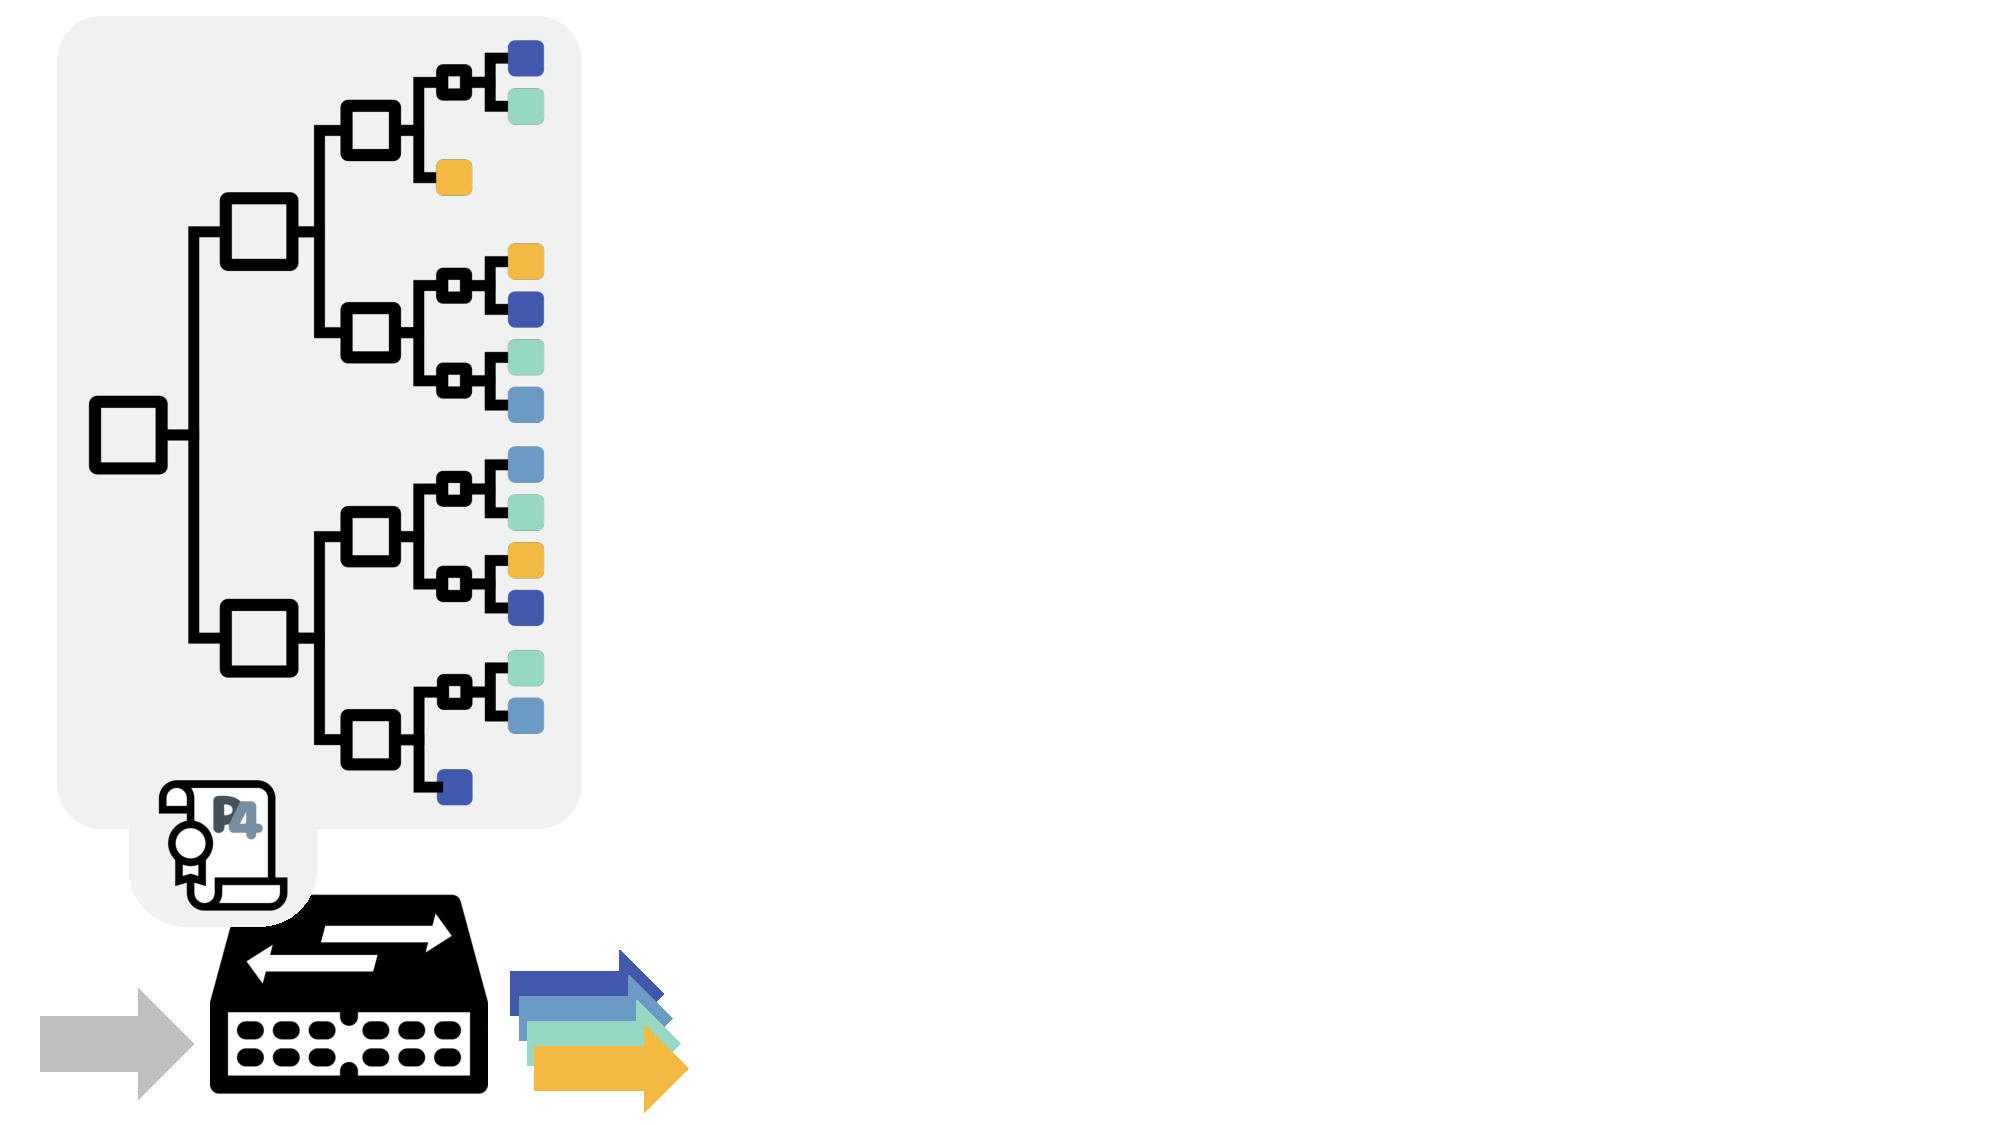
\includegraphics[height=0.5\columnwidth,trim={0 0 600pt 0},clip]{figures/monolithic.pdf}
    }
    \hspace*{-8pt}
    \subfloat[Distributed]{\label{fig:concept-distributed}
        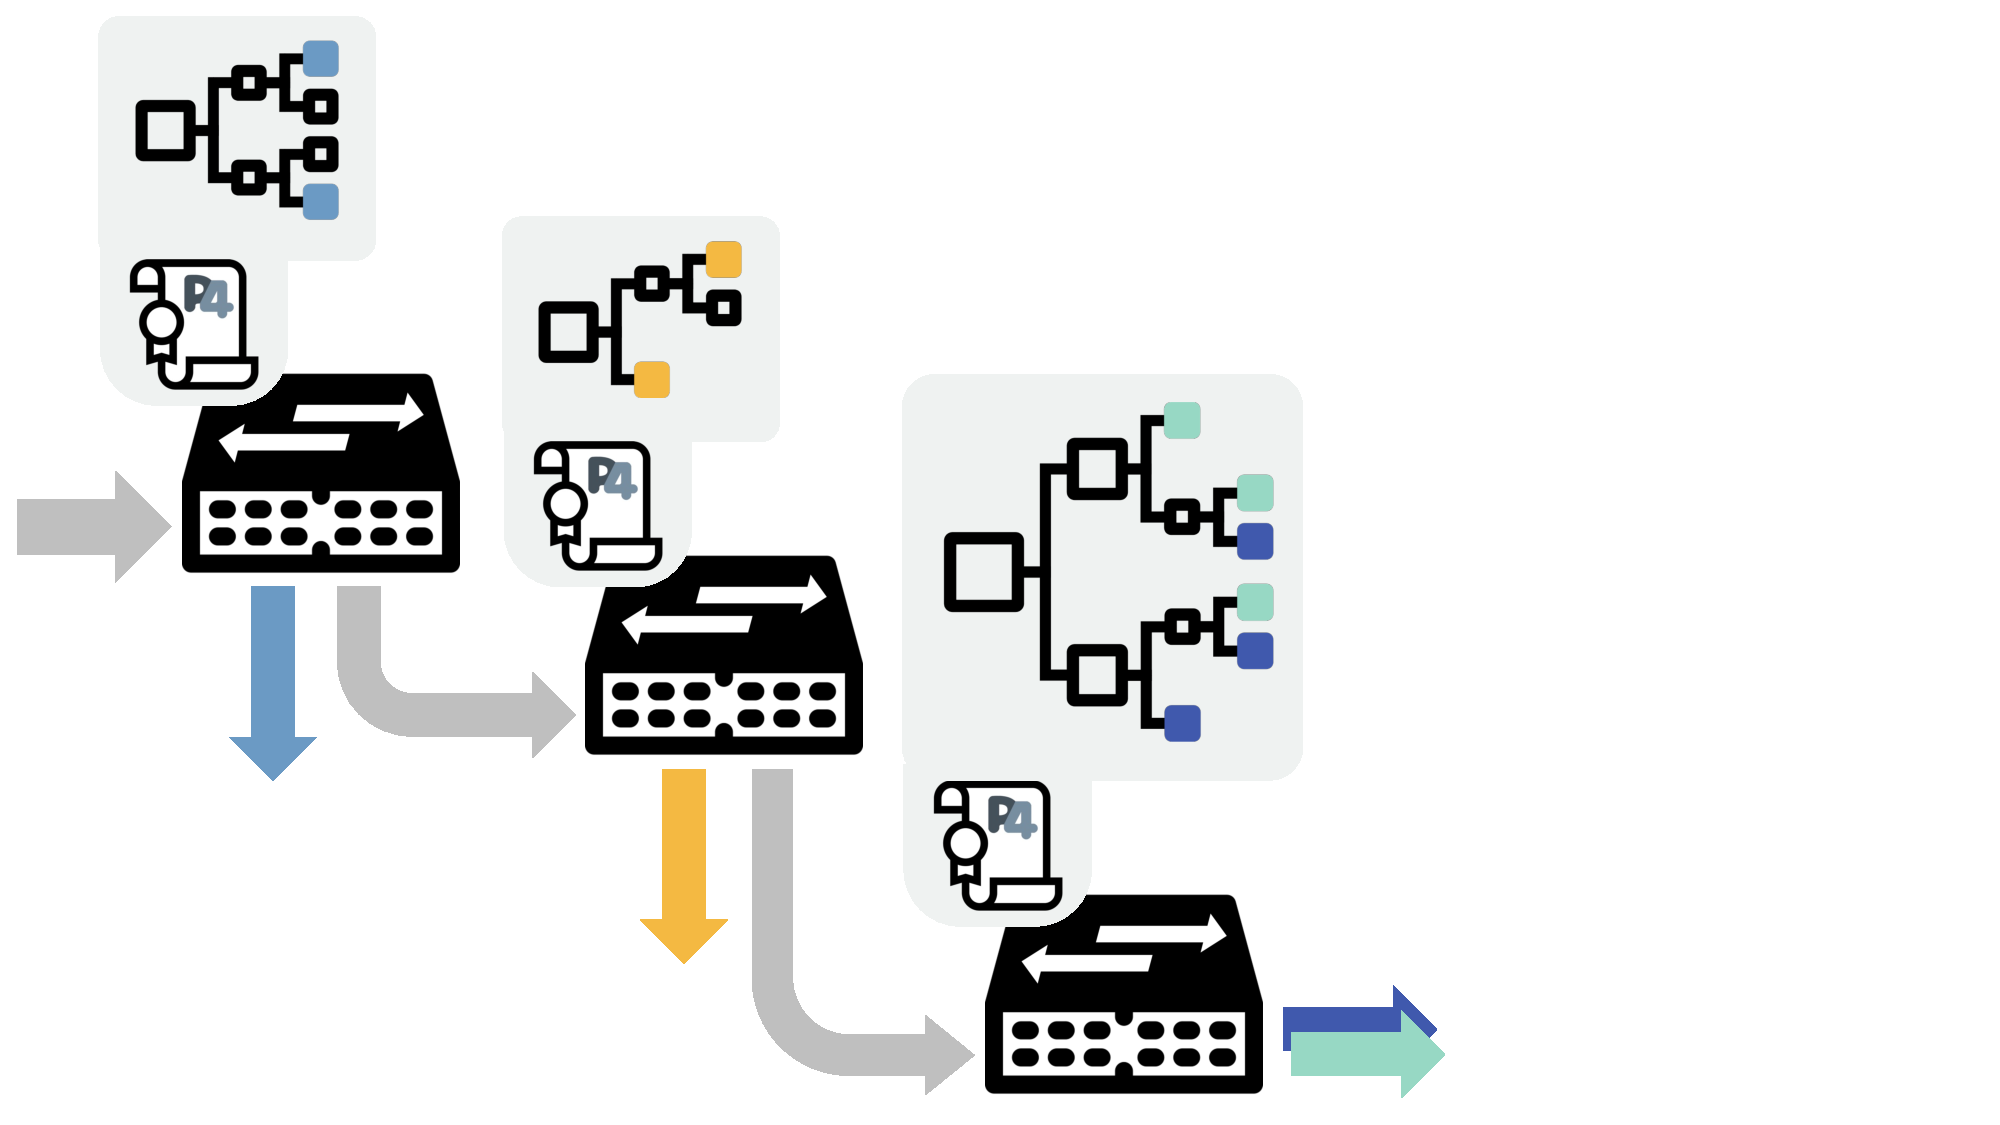
\includegraphics[height=0.5\columnwidth,trim={0 0 270pt 0},clip]{figures/distributed.pdf}
    }
    \caption{Conceptual illustration of (a) traditional monolithic and (b) proposed distributed user-plane inference strategies.}
    \label{fig:concept}
    \vspace*{-9pt}
\end{figure}

% \begin{figure}
%     \centering
%     \hspace*{-8pt}
%     \subfloat[Monolithic]{\label{fig:concept-monolithic}
%         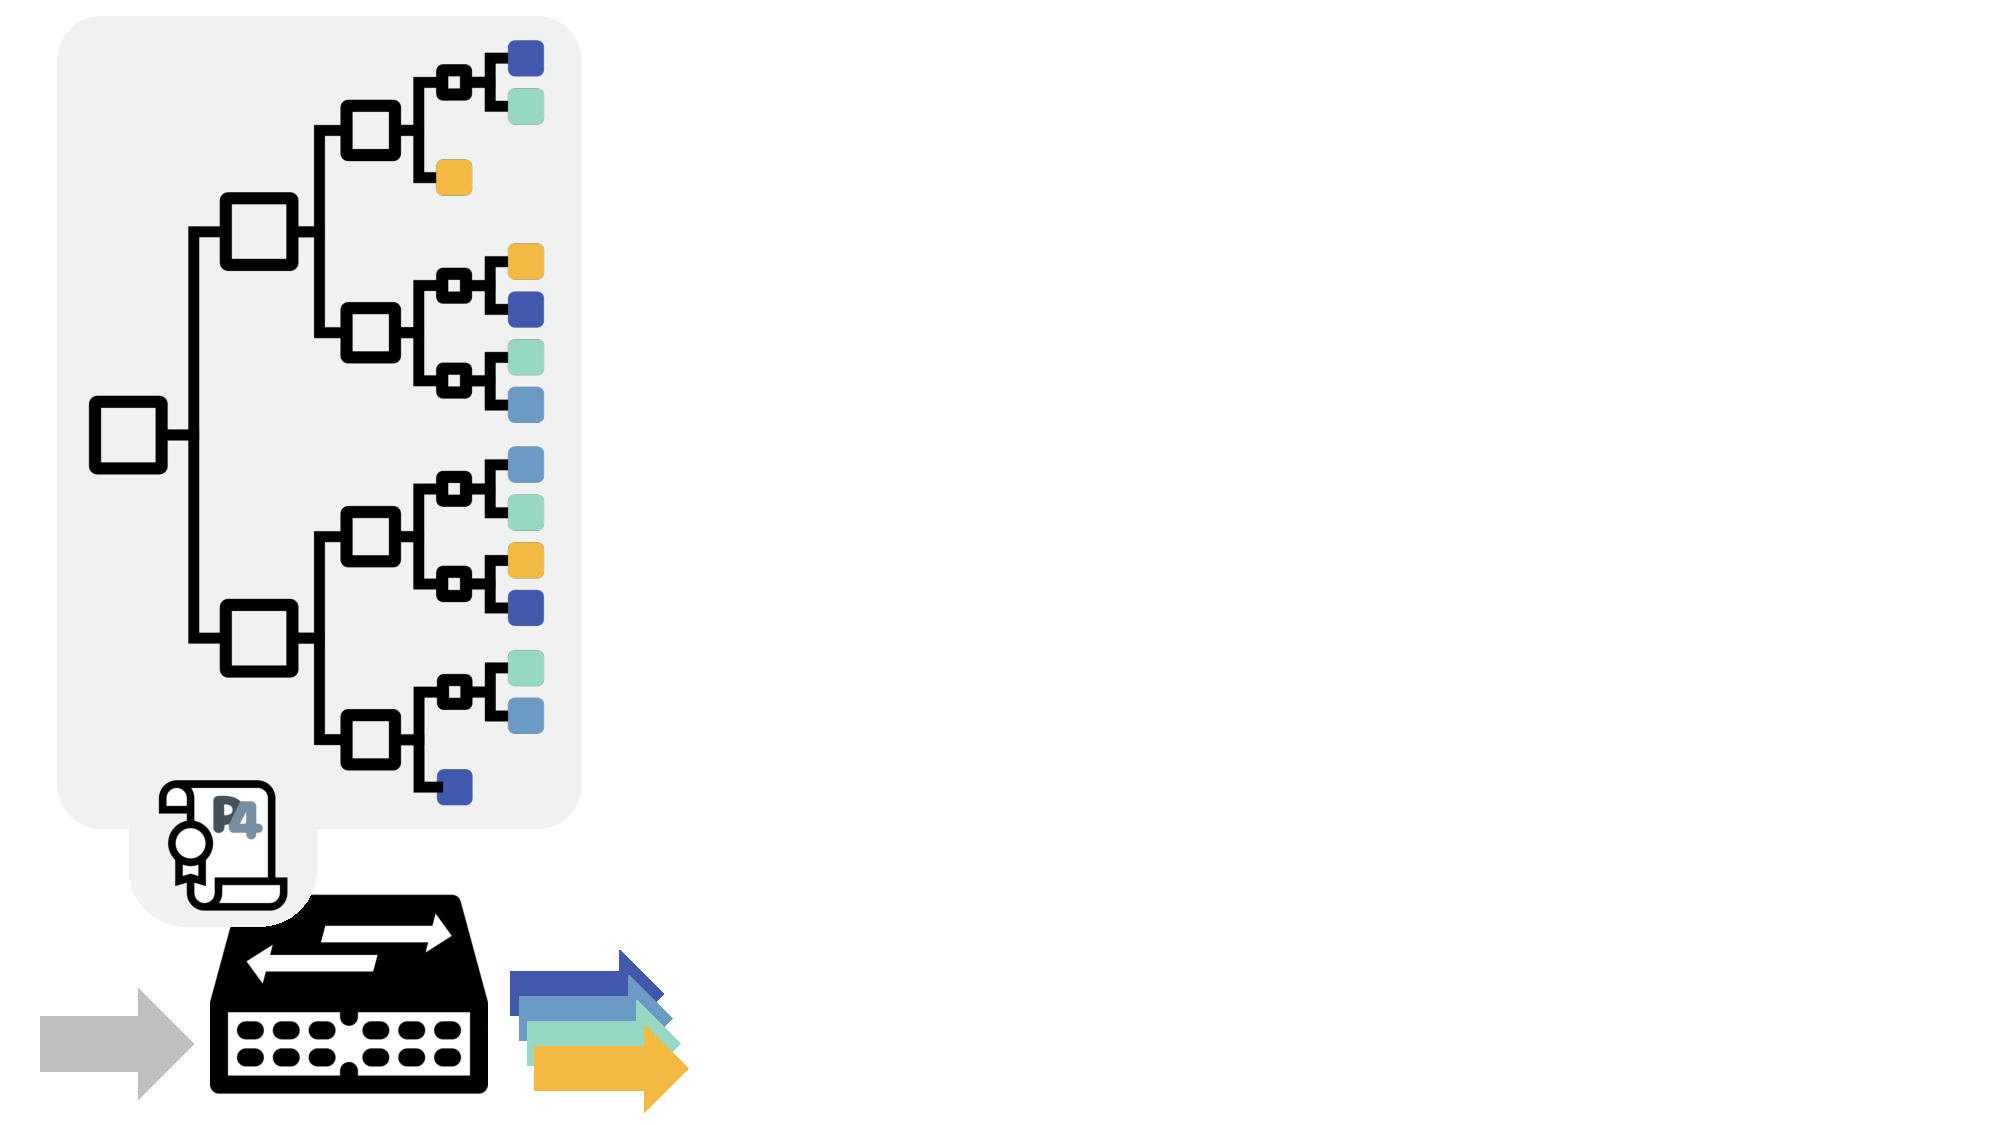
\includegraphics[height=0.5\columnwidth,trim={0 0 600pt 0},clip]{figures/monolithic.pdf}
%     }
%     \hspace*{-8pt}
%     \subfloat[Distributed]{\label{fig:concept-distributed}
%         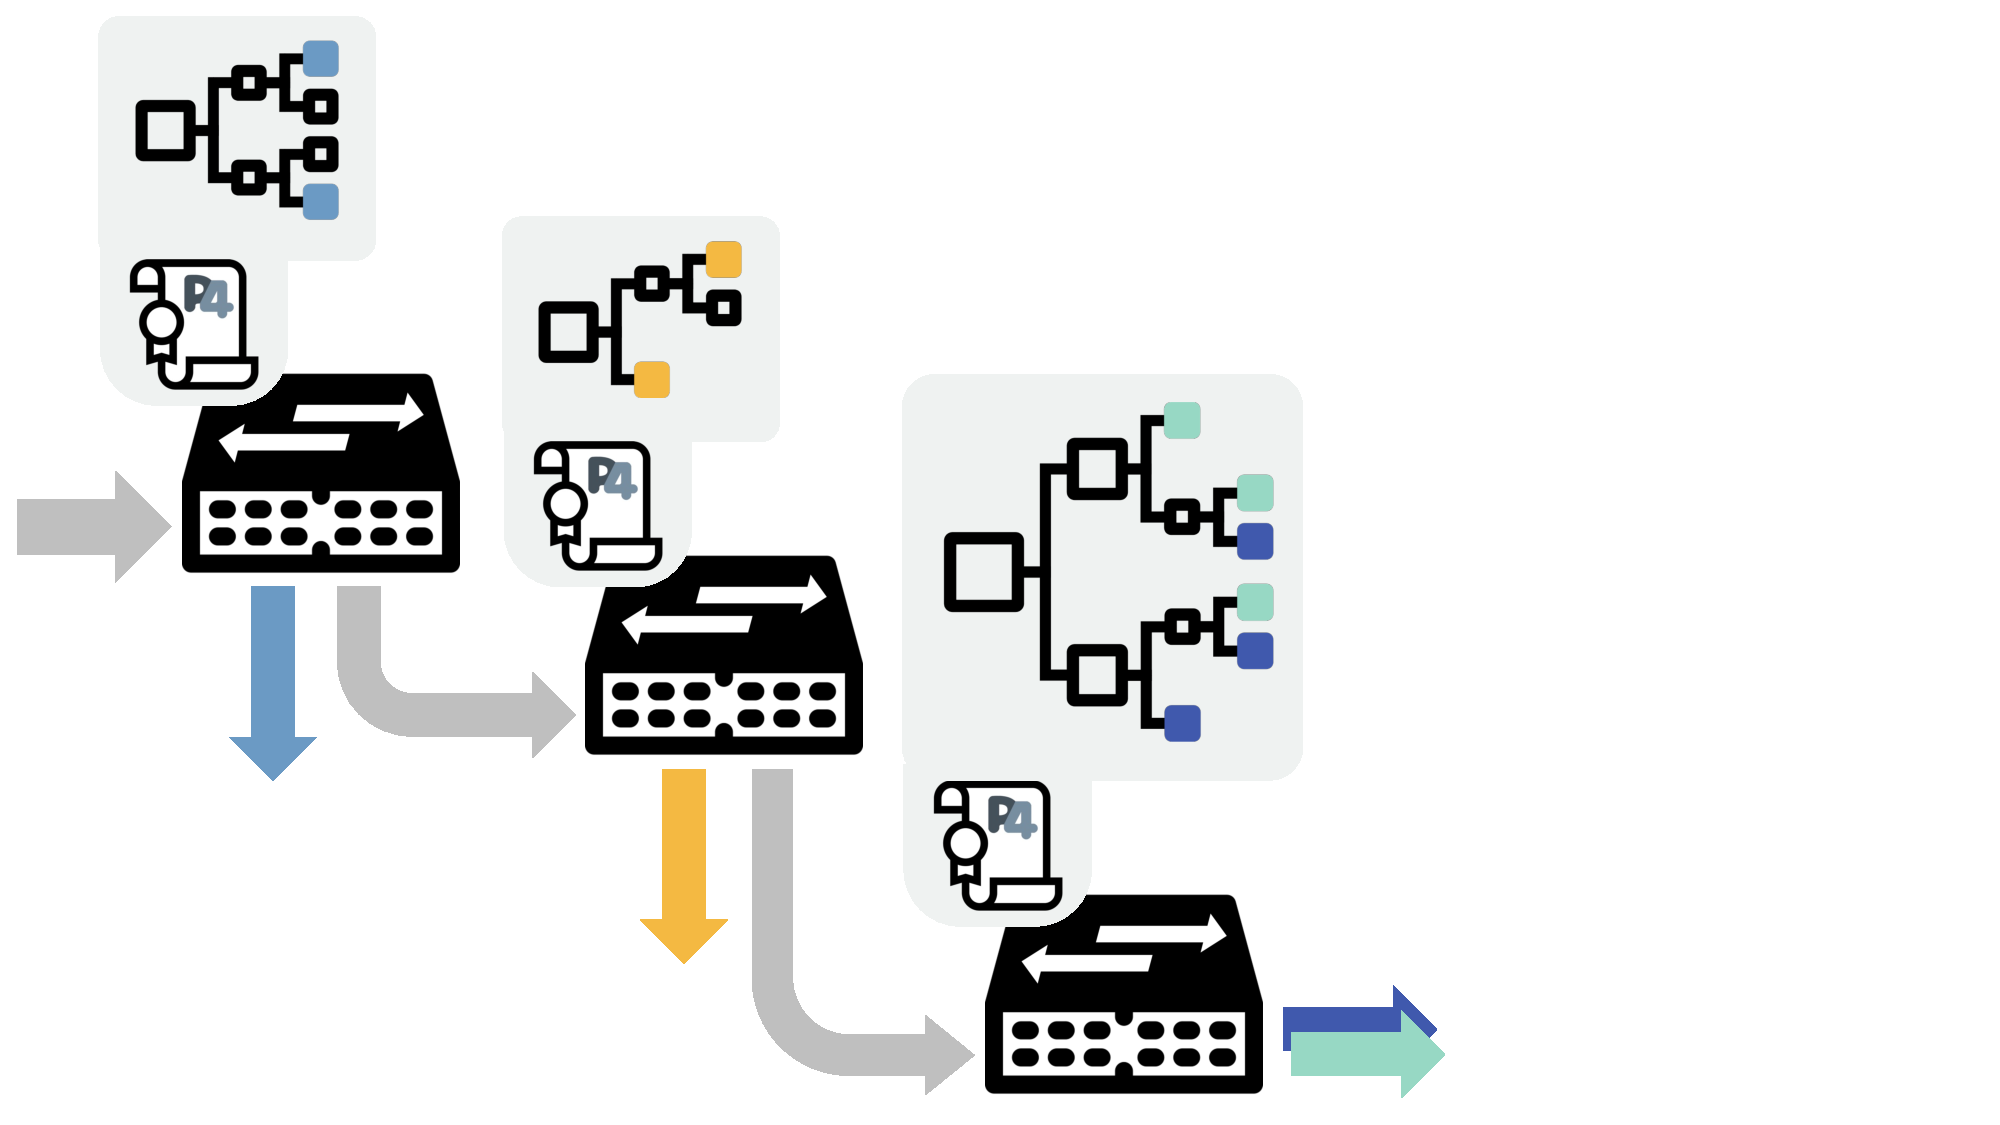
\includegraphics[height=0.5\columnwidth,trim={0 0 270pt 0},clip]{figures/distributed.pdf}
%     }
%     \caption{Conceptual illustration of (a) traditional monolithic and (b) proposed distributed user-plane inference strategies.}
%     \label{fig:concept}
%     \vspace*{-8pt}
% \end{figure}

Although the idea is conceptually straightforward, its practical realization raises several non-trivial challenges. Key challenging and open questions include how to decompose the original ML model in a way that preserves inference accuracy while keeping the resource footprint of each sub-model manageable, how to determine an optimal ordering of the resulting sub-models, and how to select their optimal placement on the predefined network paths in a given topology that ensures the target traffic traverses all sub-models in the correct order. Moreover, the decomposition process itself should ideally be automated and generalizable to arbitrary inference tasks. Furthermore, the deployment of distributed inference also introduces system-level challenges, such as ensuring scalability across diverse network architectures and achieving seamless integration with existing control and forwarding mechanisms.

% While the concept is simple, its realization poses a number of challenges. How to best decompose the original ML model in order to preserve accuracy while keeping the sub-model resource usage under control, how to order the resulting sub-models, and how to ensure automation of such a decomposition process for any inference task are hard and open questions. \bb{Deployment of \name introduces additional challenges, such as ensuring scalability across diverse network architectures and achieving seamless integration with existing control and forwarding mechanisms.}

In this paper, we present \name%
\footnote{A preliminary version was presented at IEEE INFOCOM 2025~\cite{DUNE}.}, the first practical framework for the execution of \ul{d}istributed \ul{u}ser plane i\ul{n}ferenc\ul{e} in real-world programmable hardware. 
\name focuses on a specific type of inference, \ie classification, since this is the relevant task in the vast majority of network functions that include traffic classification, intrusion detection, application identification, spam filtering, bandwidth management, and congestion management.
%
The design, implementation, deployment, and evaluation of \name yield the following main contributions.
\begin{itemize}
    \item We propose a novel framework to decompose large ML models trained to solve complex inference tasks into simpler sub-models that jointly perform the same operation. The framework is fully automated, can be applied to any class of input ML model, and solves original optimization problems in order to preserve the inference accuracy while minimizing the complexity of the sub-models.
    % \item We introduce a design of the sub-models and of their interactions that allows executing joint packet- and flow-level inference in a distributed way across multiple programmable network devices. 
    \item We present a design for the ML sub-models and their interactions that enables distributed packet- and flow-level inference across multiple programmable network devices. To orchestrate this process, we introduce a state machine that specifies the operations executed within each switch and the state transitions they trigger.
    \item The sub-models are deployed across a given network topology with varying levels of complexity, utilizing a pre-established routing strategy, while preserving compatibility with standard network functionalities. To this end, we adapt the Planner of DINC~\cite{dinc-conext23} to our specific design so as to determine optimal deployment strategies for sub-models along predefined network paths.
    \item We implement \name using the P4 language in both emulated (\ie via the bmv2 framework~\cite{bmv2}) and hardware (\ie in Intel Tofino switches) targets. We release the full software and hardware implementations along with all experimental artifacts as open source to ensure transparency, verifiability, and reproducibility of our research~\cite{code-dune}.
    \item We run proof-of-concept experiments in a real-world industry-grade testbed with a linear topology, as well as large-scale tests in Mininet~\cite{team2017mininet} across a range of complex network topologies. Results with two challenging classification tasks based on measurement traffic traces demonstrate the feasibility of our approach in practical scenarios and its gains in terms of higher accuracy over traditional single-device monolithic approaches.
    %In particular, \name’s deployment in a hardware-based linear topology improves accuracy by up to $7.5$\% while simultaneously lowering per-switch resource consumption.
    % Extensive tests on a hardware and software experimental testbed demonstrate how distributed inference grants higher accuracy than the traditional single-device monolithic approach. The gain obtained by \name's evaluation in a linear topology in hardware is up to $7.5$\%, while also using less resources per switch. 
    %\td{add results from software}
\end{itemize}

% \td{1: Explain the novel framework. 2) Design of sub-models. 3) Deployment of sub-models in more complex topologies by using the Planner of DINC. But it has number of things not in DINC. State machine. It is available. 4)HW implementation. 4) Mention the results.}

% Deploying \name in complex topologies presents additional challenges, such as ensuring that all sub-models execute in the correct order despite varying routing decisions, and identifying an optimal deployment strategy that minimizes sub-model duplication across the network.

\section{Related work}
\label{sec:related}
User-plane inference, also referred to as in-network ML, was postulated as a viable paradigm only a few years ago~\cite{Amedeo.et.al.2017,siracusano_network_ai_acc,ilsy-hotnets19}, and has since attracted growing attention from the research community. The field is now very active, and even a recent first survey published this year~\cite{in-network-ml-survey} does not capture the substantial innovation that occurred in the past six months.

Solutions to deploy trained ML models in programmable network hardware have considered different targets, including network accelerators~\cite{Taurus.2022} and SmartNICs~\cite{N3IC.2022}, yet programmable switches stay the preferred space for user-plane inference and the focus of all research summarized next.

\noindent\textbf{Monolithic tree-based models.} The vast majority of the literature proposes models based on tree structures, \ie DTs or RFs, that are implemented in individual switches. Early solutions deal with the efficient mapping of trees to the switch Application Specific Integrated Circuit (ASIC)~\cite{pForest.2019,Planter.2021,SwitchTree.2020}, considering individual DTs~\cite{infocom2021-dt-ml,soter,netpixel,friday} or special-purpose solutions tailored to one inference task~\cite{pheavy-tnsm-2021,inc}. Subsequent works cope with the limited switch resources through knowledge distillation approaches~\cite{mousika-journal-ton23}, multi-level flow table representations~\cite{SentinelX}, %with a designed dual-threshold unsupervised decision tree model
or flattening and multiplexing of sub-trees across ALUs~\cite{Leo}.
Other enhancements include exploiting both ingress and egress stages of the switch ASIC~\cite{henna}, providing support for inference based on flow-level features~\cite{flowrest}, or considering more complex tree-based models~\cite{planter-journal-ccr24}. Moreover, recent efforts achieve joint packet- and flow-level inference by automatically selecting the best option based on stateful information about each traffic flow~\cite{jewel-infocom24,netbeacon}.
All these works invariably aim at deploying monolithic ML models that perform all inference operations, including feature extraction, state maintenance, tree traversal, and consensus resolution, in a single programmable switch.

\noindent\textbf{Monolithic neural networks.} Neural architectures are significantly more involved than DTs or RFs, and embedding them in programmable switches has proven especially challenging. Still, after early attempts~\cite{N2Net.2018} several breakthroughs have led to workable implementations that rely upon custom activation functions~\cite{rids-infocom24} or Recurrent Neural Network (RNN) architectures adapted to the limited data plane stages~\cite{brain-on-switch-nsdi24}. Recently, also compressed and restructured Convolutional Neural Network (CNN) models have been successfully demonstrated in programmable network hardware~\cite{quark}.
Again, all these approaches propose to implement one NN in one switch.

\noindent\textbf{Distributed ML.} There exist several ways in which user-plane ML-driven inference can be distributed.
In a first model, \textit{inference is distributed across planes}, with part of the process run in programmable network equipment and part in a more powerful control-plane server; several works have explored this direction~\cite{knowledge_defined_networking,switchML.2021,marina-ton24} but all assume that user-plane operations happen in the same device.
%
A second approach is the \textit{separation of feature extraction from the rest of the inference process}, with the former run in different devices than the latter; the relevant position paper~\cite{bracciale-nativeni22} still considers the ML models to be monolithic and deployed in single switches.

The third acceptation is that of our interest, and intends to \textit{distribute the operation of the ML model itself across multiple user-plane devices}, as depicted in Figure~\ref{fig:concept-distributed}. To the best of our knowledge, there are just two solutions proposed to date in this direction, \ie NetNN~\cite{netnn-iscc24} and MUTA~\cite{muta25}. NetNN deploys a NN across a programmable network by implementing different layers of the neural architecture in subsequent switches. However, it realizes a specific neural model with a precise sequence of convolutional and dense layers trained for one task, \ie intrusion detection; instead, we seek a general-purpose solution that can distribute any ML model across a given programmable network. Moreover, NetNN is only emulated with the bmv2 behavioral model that is known to simplify many of the limitations of the real-world ASICs, and may result in performance losses and a need for partial model re-design when porting the solution to actual hardware~\cite{hyojoon21p4campus}. MUTA targets instead network management by jointly addressing multiple tasks through a shared multi-task learning (MTL) model instead of deploying separate models for each task. MUTA builds an MTL network that shares layers across tasks and maps them onto programmable switches for in-network inference. However, its scalability in the number of layers is bounded by the traversed switches, and the complexity of each layer is severely curbed by the switch resources.
%, as multiplication operations are replaced with table lookups of precomputed values.
% paper sumbitted to ToN that may also be relevant:
% Twin Distributed In-Network Neural Networks and Inference Load Balancing, Liu, Wai-xi; Guo, Zhen-zheng; Cui, Yong; Li, Jin; Chen, Kong-yang; Xie, Yi; Cai, Jun; Chen, Qing-chun

\noindent\textbf{Dataplane Disaggregation.}
The concept of dataplane program disaggregation was introduced by Flightplan~\cite{sultana_flightplan_2021}, a toolchain that splits a P4 program into subprograms that can be executed across devices.
This approach allows for the combination of heterogeneous hardware to overcome the limitations of single-target execution and efficient resource usage.
While Flightplan provides a framework for automated splitting, placement, and runtime support, the splitting task relies on a manual segmentation approach.
Automating the splitting task is not straightforward nor easily generalizable, as each NF type might require specific segmentation procedures, constraints, and goals.
More recently, DINC~\cite{dinc-conext23} has also addressed the problem of distributed in-network computing. %, with special attention to routing through the network.
Like Flightplan, DINC also relies on manual markers to identify the program segments, but, unlike Flightplan, which focuses on single-path scenarios, DINC considers multiple network paths and aims to ensure service provisioning for any set of predefined routes.

\noindent\textbf{Progress beyond the state of the art.}
We present \name, a solution that can automatically disaggregate any ML model for classification so that it can be deployed over a programmable network. Our solution is practical, as its design is tailored to real-world hardware and its operation is demonstrated with industry-grade programmable switches. We stress that \name goes beyond Flightplan \cite{sultana_flightplan_2021} or DINC~\cite{dinc-conext23}, as it also
% that aim at identifying the optimal set of user-plane devices receiving the component of a distributed in-network computation task (such as the distributed ML inference we consider);
produces the task \textit{segmentation} that is an input to such solutions.

% {\color{blue} REPHRASE AND MODIFY.
%  The proliferation of commercial programmable data planes has sparked a strong interest in the possibility of running ML models at line rate on individual packets. Due to the limited memory and computational capabilities of programmable network hardware, the attention has focused on the user-plane integration of models that are designed and trained offline~\cite{DP-ML-Survey-2023}.

% Proposals differ in terms of the target network equipment and class of ML model. While several programmable user planes have been considered, \eg FPGA accelerators~\cite{Taurus.2022}, NetFPGAs~\cite{IIsy.2019}, or SmartNICs~\cite{N3IC.2020}, prior works have primarily considered programmable switch ASICs based on the Protocol Independent Switch Architecture (PISA). The reason is that switches play a central role in any network infrastructure, and augmenting them with inference capabilities maximize the flexibility of any user-plane ML-driven operation.
% %to the availability of industry-grade models with large numbers of ports with capacity of hundreds of Gbps.
% Programmable switches are thus also the focus of our work.}

% {\color{blue} 
% REPHRASE AND MODIFY.

% Due to the resource constraints related to low available memory and limited support for mathematical operations of network data plane devices, we use random forest models that ($i$) fit the architecture better and ($ii$) perform as well as or even better than more complex neural network models~\cite{why-trees-outperform_NN}.

% In table \ref{tab:related-work} we compare all the solutions that have a tree-based in-switch implementation. IIsy~\cite{IIsy.2019} proposed a DT mapping scheme where features are mapped onto separate tables and then a final table summarizes the paths to leaves on the tree. The initial prototype was only tested in emulation and on a NetFPGA~\cite{zilberman2014netfpga}. This scheme is extended in a longer version of IIsy~\cite{IIsy-new} and Planter~\cite{Planter-new,Planter.2021} to overlap feature tables over multiple trees and map the paths to leaves in a code table per tree, with hardware evaluations. Both IIsy and Planter are mainly packet-level solutions although Planter envisages the scenario of flow classification but does not provide any details.

% Mousika~\cite{mousika-infocom-22} introduces a packet-level classifier based on knowledge distillation. A teacher RF, NN or DT is trained and then distilled into a single binary decision tree (BDT). While the BDT is usually mostly compact and memory efficient, the distillation often leads to a loss of classification accuracy. Other times, the BDT could grow too large that it becomes memory-hungry. In Henna~\cite{henna}, a hierarchical two-stage classifier is proposed to tackle complex per-packet classification problems which are difficult to tackle with previous solutions. Difficult tasks are split into smaller ones that can be tackled by smaller models that are more adapted for in-switch operation. However, Henna in its current state does not support flow-level classification.

% NetPixel~\cite{netpixel} is a DT-based solution performing image classification in programmable switches. An image classifier is trained in the control plane and converted into DT rules that are installed in the switch's match and action tables. The switch extracts features from incoming packets and uses the installed DT rules to classify the images. Netpixel is a packet-level solution only tested in a software switch and has not yet been demonstrated in hardware. Soter \cite{soter} is able to identify 9 types of attacks with a solution deployed partially in the user plane and partially in the switch CPU. A packet-level DT model running in switch hardware identifies suspicious packets that are cloned and sent to a flow-level CNN in the switch CPU that classifies the attack into one of 9 attacks.

% pForest~\cite{pForest.2019} is one of the first proposals for flow-level inference in programmable switches. It proposes a mapping scheme later replicated by SwitchTree~\cite{SwitchTree.2020} where each level of a decision tree is mapped onto one M/A stage of the switch pipeline. These solutions were evaluated extensively in emulation but immediately hit scalability barriers when implemented in hardware with limitations in number of stages and the nature of logical operations. In fact, pForest only manages to implement a tree of depth 4 in hardware as opposed to several trees of depth 20 in emulation. 

% In NERDS~\cite{infocom2021-dt-ml}, authors propose a flow-level classifier evaluated in a software switch. The DT mapping scheme is based on nested if/else conditional expressions, which would not be feasible in hardware for large trees as they would possibly exhaust switch gateway resources. Map4~\cite{map4} is an extension of this work. They implement a hardware prototype into a Netronome SmartNIC (Agilio CX 2x10GbE) which alleviates the constraints of programmable switches. pHeavy~\cite{pheavy-tnsm-2021} is an ML-based heavy hitter detector based on DTs, running fully in the switch. The mapping scheme is based on sequential trees which check features using range matches and enables detection of heavy flows. While pHeavy is a hardware flow-level solution, it is not general-purpose and the sequential nature of the trees poses scalability concerns. Backorders~\cite{backorders} is a recent proposal for flow-level detection of DDoS attacks with RF models in the switch. The RF mapping scheme is similar to that of pForest~\cite{pForest.2019} with each tree level mapped onto a switch M/A stage. However, it has no hardware implementation.

% INC~\cite{inc} proposes an approach to perform flow-level botnet detection with DT ensembles. The solution builds upon a Register Recycling Manager (RRM) system that aggregates counts and summations of features over multiple packets of the same flow. The flow-level features are stored in the switch registers via CRC32 hash indexing of the flow IP address. The memory occupied is released after a hash collision if the flow has already been classified. A timeout on old flows is applied to further improve scalability. The inference is performed by applying one ternary match table for each feature and one final table where all the feature combinations leading to a botnet detection are exactly matched. The solution ultimately relies on the binary nature of the classification task to identify as benign traffic each flow that does not match with any entry in the final table. This way the authors are able to drastically reduce the memory footprint of their solution, which fits into 4 stages and consumes 3.3\% of TCAM and 10\% of SRAM. Limitations of the proposed solution lie in the flow management logic, which classifies as malicious traffic all the packets coming from an IP source, and in the final table mapping that does not consider multi-class classification. A classifier running in the control plane receives the fingerprinting from the switch and discovers new botnets.

% In~\cite{friday}, the authors propose a solution that performs flow-level ransomware detection with random forests. As their previous solution \cite{inc}, they limit the number of entries in the final table by encoding just the leaves leading to a malicious detection. Nevertheless, they introduce some improvements to reduce TCAM usage and encode large RF models. The authors apply Gray coding to the feature table codes and introduce ternary matches in the final table. With such enhancements, they manage to deploy an RF with 36 trees at depth 15, leading to a 33.33\%, 5 out of 12, 10.00\%, 6.25\%, 12.98\% and 10.94\% of available TCAM, stages, arithmetic-logic unit, hash bit, and gateway resources respectively.

% Flowrest~\cite{flowrest} proposes a complete framework for deploying RF models in programmable switches for flow-level inference. It introduces a comprehensive flow management strategy for tracking and classifying flows fully in the data plane. While it brings substantial advances in the area of in-switch inference, just like all the other flow-level solutions, it leaves several packets unclassified during the feature collection and computation phase. As such, it fails to assign a classification result to all packets.

% In NetBeacon~\cite{netbeacon}, the authors propose a hybrid solution that can classify both individual packets and flows by deploying multiple tree-based models fully into the user plane. They deploy $3$ sets of models. The first is an XGBoost model whose base classifier is a DT, that serves as a flow-size predictor. Its role is to perform a per-packet classification to identify packets that belong to short flows for which no flow-level features will be computed and stored, or long flows for which memory is allocated and flow-level features are computed. This flow-size prediction is intended to avoid wasting memory to track flows for which no flow-level classification will ever be reached. The second is a packet-level classifier which classifies all the packets of short flows, packets from flows that suffer a hash collision, and all the packets that arrive before an inference point; which is the number of packets at which a flow-level decision is made. Several inference points are identified, in order to classify a flow at different stages in its life. At each inference point, a DT is deployed to classify flows of that length. While Netbeacon's deployment of multiple models enables the classification of all packets, it raises a number of concerns. \textit{($i$) Resource consumption.} Deploying multiple models leads to substantial increases in switch resource usage. In fact, in $2$ out of $3$ of the use cases presented in Netbeacon, TCAM consumption is over 30\% of what is available. This is corroborated in our experiments where Netbeacon stands out in terms of switch resource usage. \textit{($ii$) Classification accuracy.} As per-packet classification is handled by an independent packet-level model whose accuracy is often much less than that of the flow-level models, many packets end up going through this model which does not yield the desired accuracy and hence this impacts the overall accuracy, when compared to a solution that uses a single model to classify either packets or flows, which is what we propose in} {\color{red} \textbf{X}} {\color{blue}. Moreover, Flowrest~\cite{flowrest} and pForest~\cite{pForest.2019} have demonstrated that it is mostly possible to identify an optimal number of packets at which a reasonable flow-level classification can be reached. Deploying multiple models is therefore not indispensable.
% }

% {\color{red} ADD RELATED WORK for distributed solutions.}

% \subsection{User plane inference with different models}
% \label{sub:user-plane-models}

% \subsection{RF-based in-switch inference}
% \label{sub:rf-based-in-switch}
%

% \subsection{Issues with existing solutions}
% This could be merged with the previous subsection 

\section{Distributed ML Training with DUNE}
\label{sec:name-control-plane}

As any other solution for user-plane ML~\cite{jewel-infocom24}--\cite{rids-infocom24}, \name is composed of an off-line phase for the design and training of the ML model that is run in the control plane, and an on-line phase where the trained model deployed in the programmable network performs line-rate inference on the traffic. We present in this section the first phase, and in Section~\ref{sec:name-user-plane} the second.

\subsection{Workflow overview}
\label{sub:overview}

The high-level workflow of \name during the off-line phase is outlined in Figure~\ref{fig:overview}. Here, the goal of the framework is to generate a set of ML sub-models that ($i$) are compatible with the programmable network  constraints and ($ii$) jointly execute the desired inference task in the target network.

To this end, historical measurement data about the target inference task, suitably labeled for supervised learning, is initially fed to a first ML model training stage \numO{1}. At this stage, the goal is to train the most accurate ML model possible, ignoring constraints from the programmable network hardware, and the framework can accommodate any ML paradigm, \eg deep neural architectures, support vector machines, or tree-based models, as expounded in Section~\ref{sub:unconstrained-model}. The output of stage \numO{1} is a trained, complex, monolithic model that maximizes accuracy for the target traffic analysis task.

In stage \numO{2}, the monolithic ML model is examined so as to extract values that describe the importance of each input feature (\eg packet header fields or flow-level statistics) to estimate every model output (\eg a class of network traffic). Different tools can be used to that end, as outlined in Section~\ref{sub:feature-importance}, producing an importance matrix $\pmb{W}$ that expresses the relevance of features in explaining output variables and an accuracy vector $\pmb{f}$ of the inference quality for each class.

The information in $\pmb{W}$ and $\pmb{f}$ is used in stage \numO{3} to compute a partitioning $\pmb{P}$ of the original inference task into sub-tasks. Each sub-task employs a subset of the input features to estimate a specific disjoint subset of the output variables, and the partitioning aims at creating groups of variables that can be well explained by a compact set of features. To identify the best partitioning, \name hinges upon an original optimization problem solved via an efficient heuristic, as per Section~\ref{sub:partitioning}. 

\begin{figure}
    \centering
    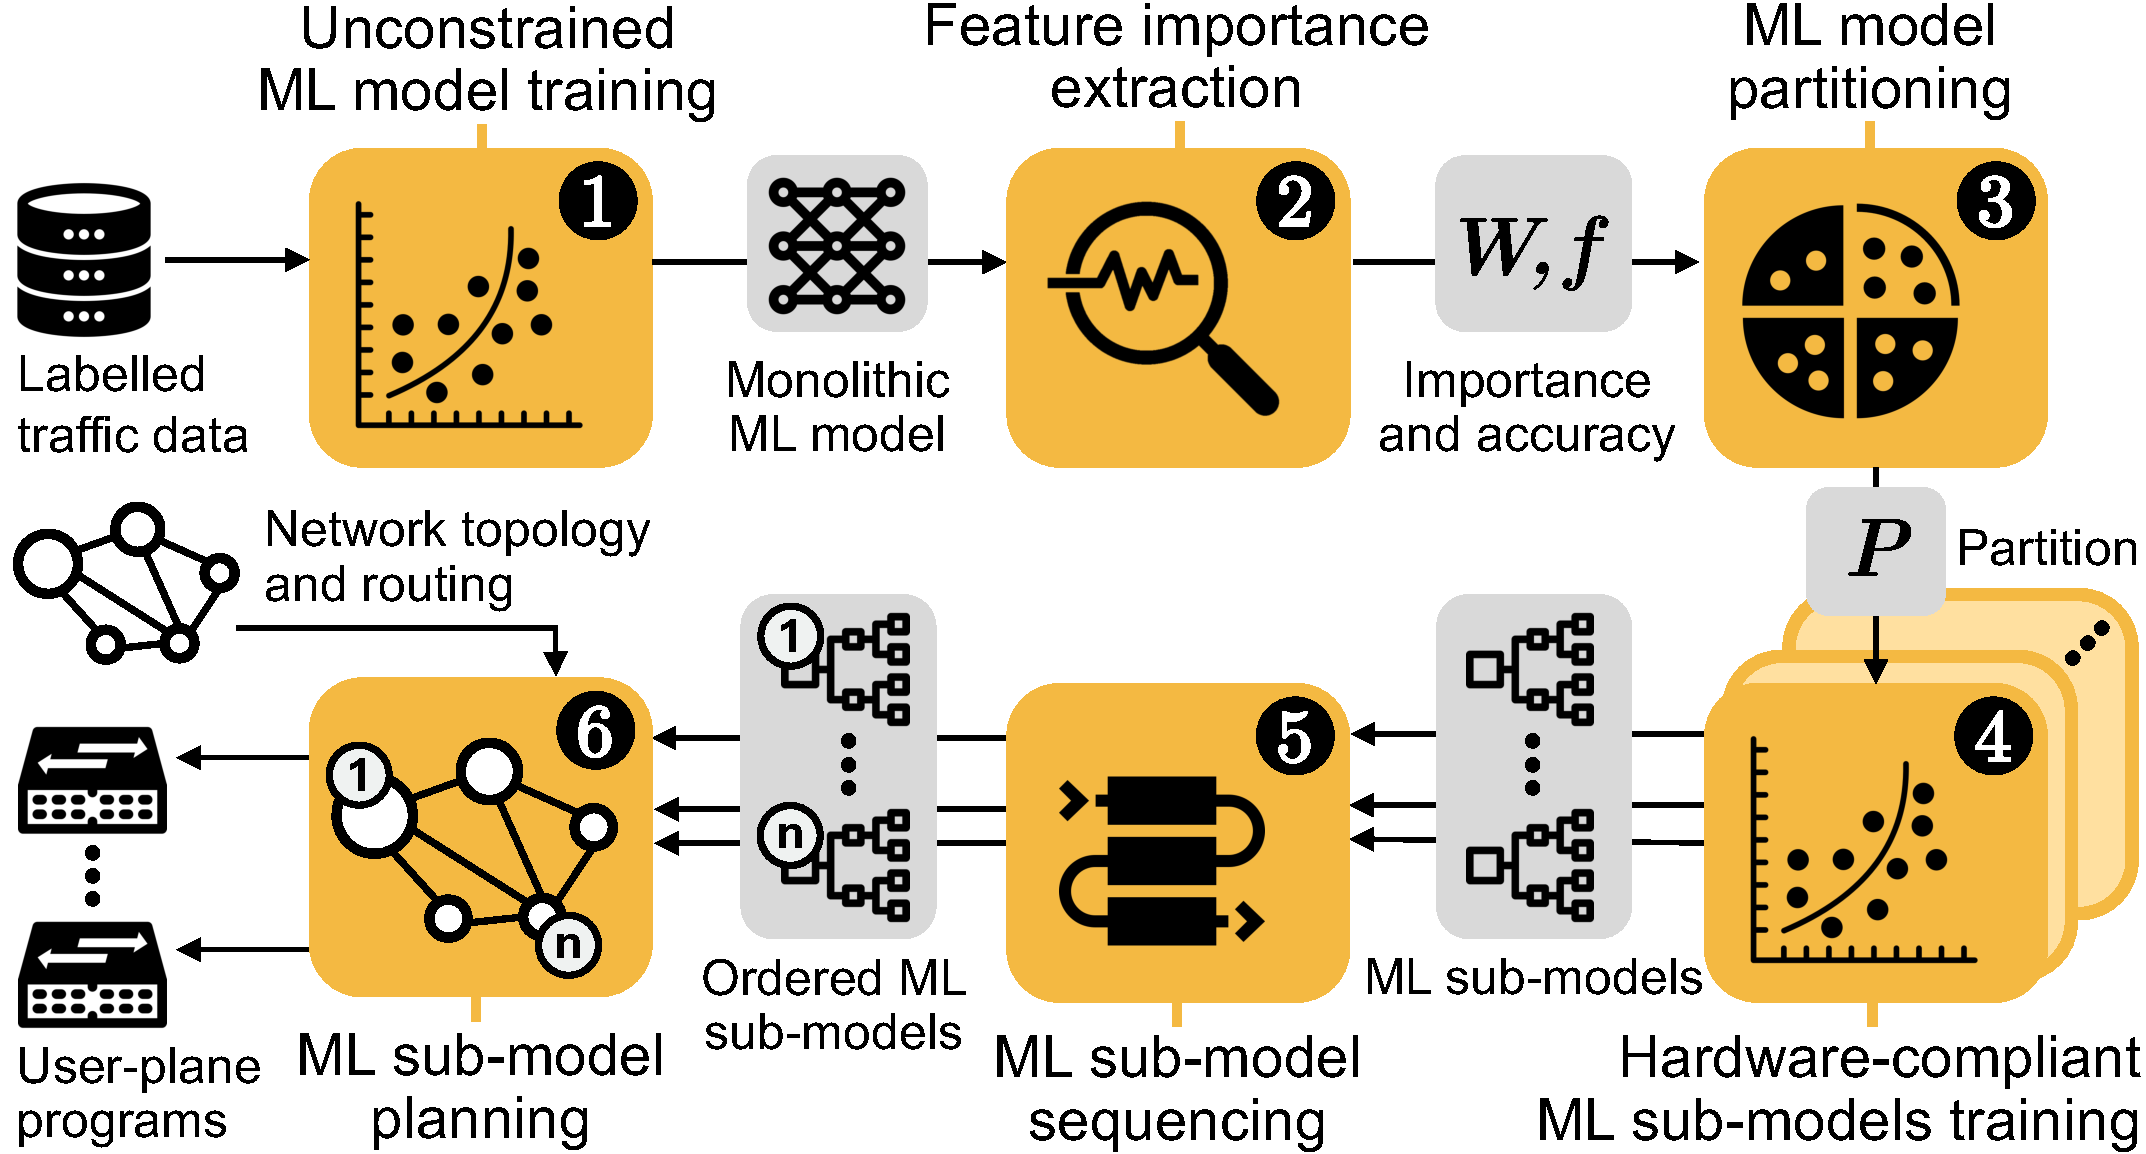
\includegraphics[width=\columnwidth]{figures/overview_v03.pdf}
    \caption{Overview of the \name workflow for the training of distributed ML compatible with programmable user planes.}
    \label{fig:overview}
    \vspace*{-8pt}
\end{figure}

For each sub-tasks in the partition $\pmb{P}$, stage \numO{4} then trains a dedicated ML sub-model that predicts the sub-task variables using the sub-task input features. In this case, the ML sub-models are designed abiding by the user-plane hardware constraints so as to ensure their compatibility with the target programmable network, as described in Section~\ref{sub:sub-models}.

As the ML sub-models tackle different portions of the whole inference task on the same network traffic, they must be run in sequence to execute the original function, similar to the chaining of Virtual Network Functions (VNFs). However, chaining ML sub-models propagates inference errors, which makes it critical to account for their (diverse) reciprocal accuracy when establishing an order of execution. As an intuitive example, it is critical to avoid deploying at the entry of the chain an ML model with a high rate of false positives: this leads to a large number of early misclassified flows, which are then never received by the downstream sub-models intended to infer the true category of such flows.
%
As discussed in Section~\ref{sub:sequencing}, the stage \numO{5} of \name solves a dedicated optimization problem based on the reciprocal accuracy of the sub-models to identify the order yielding the highest inference performance.

In the last stage, \numO{6}, the ordered sequence of ML sub-models is combined with information about the target network topology and traffic routes in order to decide how to deploy sub-models across the available switches. Specifically, the network topology and routing information are encoded as a set of available paths (\eg sequences of switches) that traffic flows may traverse. Then, an Integer Linear Program (ILP) inspired by the DINC Planner~\cite{dinc-conext23} is formulated to place sub-models to ensure that each and every packet is forwarded through sub-models in the correct order, while minimizing the number of switches where inference occurs--hence the overall user-plane resource consumption of the ML process. Full details are provided in in Section~\ref{sub:planner}.
%It is worth noting that the problem of identifying (\eg within a complex network topology) the exact devices where the sequence of ML sub-models shall be deployed goes beyond the scope of \name and can be addressed with solutions already present the literature. In fact, one can consider the ordered sub-models generated by \name as a chain of user-plane VNFs and apply one of the many algorithms proposed in the literature for VNF chaining optimization~\cite{vnf-chaining_survey}; or, regard the output of our framework as a segmentation of an in-network computation task and employ a dedicated solution like DINC~\cite{dinc-conext23}.

Finally, each ML sub-model is coded as a P4 program and injected into the target programmable user-plane devices. It is worth noting that the implementation of the sub-models into resource-constrained hardware targets is an entangled task, exacerbated by the fact that such sub-models must operate in a coherent way once distributed across any network topology and in presence of packet losses or reordering. This involves several important design decisions and a dedicated operational logic, which are discussed in Section~\ref{sec:name-user-plane}.

\subsection{Unconstrained ML model training}
\label{sub:unconstrained-model}

Stage \numO{1} consists of the definition, hyper-parametrization and training of a single ML model that solves the desired inference task. As anticipated, this model is \textit{unconstrained}, \ie is not limited by the programmable hardware memory or compute constraints; hence, can be as complex as the control-plane ML Operations (MLops) resources allow. The exclusive objective of this unconstrained ML model is achieving the maximum accuracy possible in the target inference task.

While this stage of \name is general and can accommodate different ML paradigms, in our implementation we opt for using a large RF as the unconstrained model. The motivation is twofold: first, RFs are inherently more explainable than neural architectures, making the extraction of feature importance from a trained model much faster and more precise, as explained in Section~\ref{sub:feature-importance}; second, for the challenging traffic classification use cases employed to evaluate the performance of \name and presented later in Section~\ref{sec:experimental-setup}, using NNs based on Mutit-Layer Perceptron (MLP) as the unconstrained ML models returned sensibly lower accuracy than that of RFs.
%third, using an RF allows for a more direct comparison against solutions in the literature that adopt monolithic RFs to perform user-plane inference.

To design the unconstrained RF, we start from the RF model recently proposed by Jewel~\cite{jewel-infocom24}, a tree-based architecture that can perform packet-level inference (\ie using only features extracted from the header of the current packet, such as payload length) on the first packets of a flow and automatically switch to a more accurate flow-level inference (\ie using features that relate to all received packets in the same flow, such as the average inter-arrival time) as soon as enough packets in the flow  have been seen to build reliable flow statistics. Note that we consider the monolithic version of this type of tree that is originally implemented in Jewel as a benchmark in the comparative evaluation in Section~\ref{sec:evaluation}.

\name hyper-parametrizes the joint packet- and flow-level RF model by training it with an exhaustive grid search over the space of hyper-parameters, \ie the maximum number of trees, the maximum depth of each tree, and the rank of the packet for which the flow-level inference is triggered. The grid search is iterated so as to also identify the optimal set of input features that maximizes the unconstrained model accuracy: specifically, we start from a model trained with the full set of all available features, compute the Mean Decrease in Impurity (MDI) to remove the least relevant feature, re-run the grid search, and iterate. In the end, we select the RF model that achieves the highest \textit{macro F1} score (see Section~\ref{sub:metrics} for a definition).

\subsection{Feature importance extraction}
\label{sub:feature-importance}

% \mf{Note that we can present \name as a general framework for \textit{any} ML model, \ie the original monolithic model does not need to be a RF; it could be, \eg a NN on which we run SHAP to get the importance of features per class. Then, of course, the sub-models are RFs. In our tests we use an RF as the monolithic model, but the framework is in fact more general and Figure~\ref{fig:overview} shall reflect that.}

Stage \numO{2} extracts the relationships between input features and output variables from the unconstrained model produced by the previous stage. It is worth highlighting that here we do not seek to rank the importance of the input features for the inference task as a whole, for which standard techniques such as the MDI used in stage \numO{1} exist. Instead, we need to quantify the explanatory power of each input feature for each individual output class, which is a sensibly harder problem.

\name takes advantage of the design choice of adopting an RF model in stage \numO{1} to extract feature importance efficiently. Specifically, it leverages the Per-Class Feature Importance (PCFI) method~\cite{Cramer_Per-Class_Feature_Importance_2020}, which operates on tree structures and extends MDI by considering the paths (\ie sequences of nodes from the root node to a leaf that contains the inference decision) that compose the trained RF. For each path in every RF tree, PCFI calculates the importance of a given feature as the total MDI at nodes that split their sub-trees based on that feature; it then associates such an MDI value to the class in the leaf at the end of the path. Once all paths have been processed, PCFI computes the final importance values for a feature-class pair as the mean of all MDI values of the input feature associated with the target class.
%The time complexity of the given approach is $O($\var{t}$\cdot$\var{L}$\cdot$\var{d}$)$, where \var{t}, \var{L}, and \var{d} represent the number of trees in the Random Forest model, maximum number of leaves in a tree, and the maximum depth of each tree.

The PCFI approach is not the only one possible. For instance, the well-known SHapley Additive exPlanations (SHAP)~\cite{NIPS2017_8a20a862} offer an alternative way to derive from a trained model how much each input feature contributes to the inference of an individual output variable. SHAP computes so-called Shapley values for each feature and produced inference output by evaluating all possible permutations of the features and determining the marginal contribution of the feature to the prediction as the difference caused by its absence.
While SHAP has the advantage of being applicable to any ML model, it suffers from poor exponential scalability in the model complexity~\cite{arora2009computational} that makes it impractical in many cases.

In the case of tree-based models, a compute-efficient variant of SHAP exists: TreeSHAP~\cite{treeSHAP} leverages the structure of trees to compute exact Shapley values in polynomial time.
%TreeSHAP calculates feature importance for individual data points by leveraging the structure of decision trees, recursively determining each feature's contribution based on the paths taken from the root to the leaf nodes. It aggregates these contributions across all trees in an ensemble to provide the final SHAP values. The computational complexity of the TreeSHAP algorithm per individual data point is $O($\var{t}$\cdot$\var{L}$\cdot \var{d}^2)$, where \var{t}, \var{L}, and \var{d} represent the number of trees in the Random Forest model, maximum number of leaves in a tree, and the maximum depth of each tree.
Yet, the complexity of PCFI and TreeSHAP is still very different. Let us denote by \var{t}, \var{L}, and \var{d} the number of trees, the maximum number of leaves in a tree, and the maximum depth of each tree in the unconstrained RF model, respectively: then PCFI has a complexity $O($\var{t}$\cdot$\var{L}$\cdot$\var{d}$)$ whereas that of TreeSHAP is $O($\var{t}$\cdot$\var{L}$\cdot \var{d}^2)$.
As tests with the reference use cases in Section~\ref{sec:experimental-setup} show similar accuracy in the feature importance returned by PCFI and TreeSHAP, we opt for the former in our implementation.
% Since features with low importance values have a minimal impact on the classification of specific classes, we focus on the most significant features for each class during clustering. Our objective is to identify outlier features and select the most important feature set for each class. This selection is based on maximizing the cumulative feature importance calculated over the selected features while considering the cost of each feature selection, as shown below:
%
% \begin{equation}
% \begin{array}{rrclcl}
% \displaystyle \max_{I} & f($i$) = {\sum_{i \in I} {U_{i}}-\sum_{i \in I} {C_{i}}}\\
%
% \end{array}
% \end{equation}
% ,where \textit{I} is the set of features, $U_{i}$ is the importance value of the feature \textit{i}, and $C_{i}$ is the cost of selecting that feature. The feature set \textit{I} of increasing size (ranging from $1$ to the total number of features used in the main model) is generated by sequentially including features, starting with the most important. The cost of selecting each feature is determined as the reciprocal of the total number of features used in the main model.
%
% \bb{Add some plots of outlier detection function.}
\subsection{ML model partitioning}
\label{sub:partitioning}

Stage \numO{3} breaks down the original inference task into a series of smaller sub-tasks that jointly achieve the same goal. To this end, \name solves an original Set Partitioning Problem (SPP) to identify sub-tasks as disjoint groups of output classes that can be explained with high accuracy by a compact set of input features each. We next formalize SPP as an optimization problem and present the efficient heuristic used to solve it.

\vspace*{4pt}
\subsubsection{Formulation}
Let $V=\{v_1,\dots,v_m\}$ be the set of all $m$ output variables (\ie classes) that must be explained with the set of $r$ features in the inference task. Also, let us denote by $S=\{S_1,\dots,S_n\}$ the set of all possible blocks (\ie class groups). $P \subset \{1,\dots,n\}$ is a partition of $V$ if and only if
\begin{equation}
    \bigcup_{i\in P}S_{i}= V \quad \text{and} \quad
    S_i \cap S_j = \emptyset \quad \forall i,j \in P, i\neq j.
    \label{eq:opt-constraints}
\end{equation}

The goal of the SPP is to find the partition $P$ that best balances inference accuracy and programmable network resource use. This translates into the two following requirements.
\begin{itemize}
    \item[($i$)] \textit{Compactness}. $P$ shall be formed by the smallest possible number of blocks. This requirement stems from the fact that each block will be later mapped by our framework into a separate ML sub-model, and every added sub-model yields overhead (as it requires, \eg maintaining its own flow state registers or mapping its ML logic to a user-plane device) and grows the number of network devices required to implement the full distributed solution.
    \item[($ii$)] \textit{Effectiveness}. Each block in $P$ shall maximize the accuracy of inference for the variables it includes by using a minimum number of features. The rationale is that accuracy must be preserved with limited feature sets, which later translate in less complex ML sub-models.
\end{itemize}
It is worth noting that the two requirements above entail a clear trade-off: the best accuracy using small feature sets is achieved with tiny blocks each dedicated to very few variables; yet, that also creates a large number of ML-models, which ultimately harms resource usage. The SPP thus aims at finding the best partition that solves such a trade-off.

The optimization problem can be formalized using a matrix representation.
Let $\pmb{s}_i \in \mathbb{Z}_2^m, i \in \{1,\dots,n\}$ be an indicator vector designating which variables in $V$ are part of a block $S_i$, \ie the $k$-th element of $\pmb{s}_i$ is $1$ if class $k$ is in $S_i$ and $0$ otherwise. We then construct a matrix $\pmb{A} \in \mathbb{Z}_2^{m \times n}$ with the $\pmb{s}_i$ vectors as the $n$ columns.
By defining a vector of binary decision variables $\pmb{x} \in \mathbb{Z}_2^n$ whose $i$-th element indicates if a block $S_i$ is selected as part of the output partition $P$, we can write the constraints in \eqref{eq:opt-constraints} as $\pmb{Ax}=\pmb{1}$.
%
The formal definition of the optimization problem is then
\begin{equation}
\max_{\pmb{x}} \; \frac{1}{c(\pmb{x})}\cdot\pmb{g}^T\pmb{x} \qquad \text{s.t.} \quad \pmb{Ax}=\pmb{1},
\label{eq:opt-objective}
\end{equation}
where $c(\pmb{x})$ captures requirement ($i$) above and denotes the cost of partitioning the inference task into the number of blocks defined by $\pmb{x}$, whereas $\pmb{g}^T\pmb{x}$ models requirement ($ii$) as the accuracy achieved for the blocks in $\pmb{x}$ with minimum features.

More precisely, the cost $c(\pmb{x})$ is expressed as
\begin{equation}
    c(\pmb{x})=\frac{m-1}{m-\pmb{1}_n^T\pmb{x}},
    \label{eq:opt-cost}
\end{equation}
where $\pmb{1}_n\in\mathbb{Z}_2^n$ is a vector of $1$'s hence $\pmb{1}^T\pmb{x}$ is a scalar corresponding to the number of non-zero elements of $\pmb{x}$, \ie the number of blocks in the selected partition. This entails a linearly decreasing advantage $1/c(\pmb{x})$ as the number of blocks grows up to the total number of variables $m$.

As far as the second factor of the objective function in~\eqref{eq:opt-objective} is concerned, $\pmb{g} \in \mathbb{R}^n$ is a vector of the gains $g_i$ associated with all of the possible blocks $S_i$, which is expressed as
\begin{equation}
    g_i = \Theta(\pmb{s}_i) \cdot \Psi(\pmb{s}_i), \quad\text{where}\label{eq:opt-gain}
\end{equation}
%where
\begin{eqnarray}
    \Theta(\pmb{s}_i) &=& \max_{\pmb{\phi}} \quad \pmb{s}_i^T\pmb{W\phi} - (\tfrac{1}{r}(\pmb{1}_n^T\pmb{s}_i)\pmb{1}_r)^T\pmb{\phi} \label{eq:opt-gain-theta} \\
    \Psi(\pmb{s}_i) &=& 1/(1 + \hspace*{-8pt}\max_{v_k|\pmb{s}_i(k)=1} \hspace*{-8pt} f_k - \hspace*{-8pt}\min_{v_k|\pmb{s}_i(k)=1} \hspace*{-8pt} f_k). \label{eq:opt-gain-psi}
\end{eqnarray}

In the expression in~\eqref{eq:opt-gain-theta}, the matrix $\pmb{W}\in\mathbb{R}^{m \times r}$ contains the per-class feature importance values returned by stage \numO{2},
%consists of $m$ distributions of weights (importance) $W_a=\{w_a^1,\dots, w_a^r \mid \sum_{i=1}^r w_a^i = 1 \}$, where $a$ denotes one class $C_a$. Letting $\pmb{w_a}$ be a vector representation of such set, we construct the matrix $\pmb{W}$ using them as rows.
while $\pmb{\phi} \in \mathbb{Z}^r_2$ is an array denoting a feature subset, \ie the $h$-th element is $1$ if feature $h$ is in $\pmb{\phi}$, and $0$ otherwise. Then, $\pmb{s}_i^T\pmb{W\phi}$ is the cumulative importance retained by the selected features in $\pmb{\phi}$ for classes in $S_i$, whereas $(\tfrac{1}{r}(\pmb{1}_n^T\pmb{s}_i)\pmb{1}_r)^T\pmb{\phi}$ is a penalty on the number of features used to achieve such importance.

In~\eqref{eq:opt-gain-psi}, $f_k$ is the $k$-th element of array $\pmb{f}\in\mathbb{R}^n$ provided by stage \numO{2} and denotes the accuracy (\eg the F1 score defined in Section~\ref{sub:metrics}) achieved by the unconstrained ML model in inferring class $v_k$.
The expression introduces a penalty proportional to the maximum difference in accuracy for two variables in the block $S_i$: high differences indicate inherent diverse complexity of the inference process for the corresponding classes, which in turn suggests that such classes need ML sub-models of sensibly different size and are thus not good candidates for grouping.

\vspace*{4pt}
\subsubsection{Solution}
%\mf{David, can you explain here that the problem in~\eqref{eq:opt-objective} cannot be solved, and explain how you solve it with a greedy approach, including the efficient calculation of~\eqref{eq:opt-gain-theta}? Add plots (\eg annotated dendograms, toy examples or similar) if you think that they help understanding the process}
The SPP is known to be NP-hard even in its basic optimization problem formulation where the objective function is linear in the decision variables $\pmb{x}$. Yet, in that case, the SPP can be rendered as an Integer Linear Problem (ILP) and solved using standard solvers up to a reasonable size.
Unfortunately, the objective function in~\eqref{eq:opt-objective} is non-linear, impeding such a simplification and making an optimal solution computationally impractical.
% Alternatively, it is possible to penalize blocks with fewer classes so that solutions including fewer blocks are preferred. However, this has a local effect instead of a global effect that the compactness factor introduces. (Maybe for discussion?)

% \newlength{\oldtextfloatsep}\setlength{\oldtextfloatsep}{\textfloatsep}
% \setlength{\textfloatsep}{0pt}

\begin{algorithm}[tb]
\caption{SPP greedy algorithm.}
\label{alg:greedy}
\begin{algorithmic}[1]
\small
\Require $\textit{fix\_level} \in \{2, \dots, m\} \cup \{\emptyset\}$
\State $\textit{level} \gets m$, $\textit{gain} \gets 0$, $(\textit{blocks}) \gets \text{all single-element blocks}$
\For{$i = m, \dots, 2$} \label{alg:for-m}
    \State $\textit{tuples} \gets \Call {combinations}{\textit{blocks}, 2}$ 
    % \State $\textit{gains} \gets [ ]$
    \ForAll{$ \textit{tuple} \in \textit{tuples}$} \label{alg:for-gains-begin}
        \State $\textit{gains} \gets \Call {computeBlockGain}{\textit{tuple}}$ %\Comment{\textcolor{blue}{includes feature selection}}
    \EndFor \label{alg:for-gains-end}
    \State $\textit{best tuple} \gets argmax(\textit{gains})$ \label{alg:gain-max}
    \ForAll{$\textit{block} \in \textit{blocks}$} \label{alg:for-update-begin} %\Comment{\textcolor{blue}{remove invalidated blocks}}
        \ForAll{$\textit{element} \in \textit{best-tuple}$}
            \If{$\textit{element} \in \textit{block}$}
                \State $\Call{remove}{\textit{element}, \textit{blocks}}$
            \EndIf
        \EndFor
    \EndFor
    \State $\Call{add}{\textit{best-tuple}, \textit{blocks}}$ \label{alg:for-update-end}
    \State $\textit{gain} \gets \Call{computePartitionGain}{blocks}$ \label{alg:store-max-begin}
    \If{$\textit{gain}>\textit{gain-max}$}
        \State $\textit{level} \gets i$
        \State $\textit{gain-max} \gets \textit{gain}$
    \EndIf \label{alg:store-max-end}
\EndFor
\end{algorithmic}
\end{algorithm}
% \setlength{\textfloatsep}{\oldtextfloatsep}

We propose a greedy approach, summarized in Algorithm~\ref{alg:greedy}, to approximate~\eqref{eq:opt-objective}.
The algorithm mimics an agglomerative clustering process where the gain in~\eqref{eq:opt-gain} is used as the \textit{similarity metric} to merge at every iteration the two (blocks of) variables with maximum similarity.
The algorithm performs $m-1$ iterations (line~\ref{alg:for-m}); at each iteration, it computes gains%
\footnote{Gains calculated at a previous iteration are cached and not re-computed.}
among all current blocks (lines~\ref{alg:for-gains-begin}--\ref{alg:for-gains-end}), identifies the pair of blocks with maximum gain (line~\ref{alg:gain-max}), and updates the blocks data structure with the new merged block (lines~\ref{alg:for-update-begin}--\ref{alg:for-update-end}).
%
Each iteration returns a partition whose total gain is computed using~\eqref{eq:opt-objective} and possibly stored as the maximum gain achieved (lines~\ref{alg:store-max-begin}--\ref{alg:store-max-end}).
Such gains are not monotonic in general with respect to the iterations, but take different shapes depending on the target inference task. Figure~\ref{fig:blocks_selection} shows the evolution of the gain matching our objective function~\eqref{eq:opt-objective} over iterations, for one of the reference use cases we will present in Section~\ref{sec:experimental-setup}.

The computation of the gain in~\eqref{eq:opt-gain} needs to be especially efficient since it is profusely used in Algorithm~\ref{alg:greedy}, hence we propose a computationally viable implementation with cost $O(r)$. The gain is a product of~\eqref{eq:opt-gain-psi} and~\eqref{eq:opt-gain-theta}: while the factor in~\eqref{eq:opt-gain-psi} is inexpensive, we decompose the calculation of~\eqref{eq:opt-gain-theta} into $r$ sub-problems leveraging its structure.
In each of sub-problem, a feature is selected if the importance gain, \ie the minuend in~\eqref{eq:opt-gain-theta}, overcomes the uniform penalty, \ie the subtrahend in~\eqref{eq:opt-gain-theta}.
For example, Figure \ref{fig:feature_selection} shows in green the features with a positive net importance gain for a given block $s_i$ of the SPP for to the same inference task of Figure~\ref{fig:blocks_selection}.

\begin{figure}
    \centering
    \vspace*{-16pt}
    \subfloat[Blocks selection]{\label{fig:blocks_selection}
    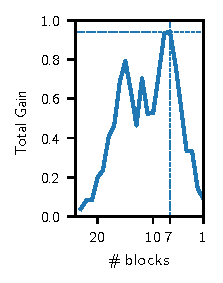
\includegraphics[height=0.55\columnwidth,trim={0 5pt 0 0},clip]{figures/plot_block_selection.pdf}
    }\hspace*{-12pt}
    \subfloat[Feature selection]{\label{fig:feature_selection}
    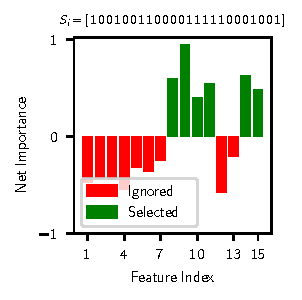
\includegraphics[height=0.55\columnwidth,trim={0 5pt 0 0},clip]{figures/plot_feat_selection.pdf}
    }
    \caption{Greedy solution to the SPP in~\eqref{eq:opt-objective} in the UNSW use case. The plots show (a) the gain versus the number of blocks and (b) the feature selection for a given block $S_i$.}
    \label{fig:greedy}
    % \vspace*{-4pt}
\end{figure}

\begin{figure}
    \centering
    \subfloat[Gain performance]{\label{fig:gain-performance}
        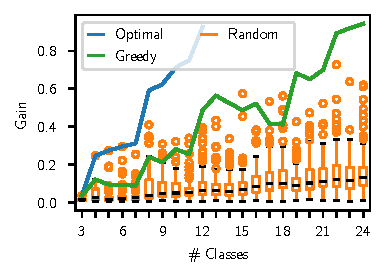
\includegraphics[height=0.5\columnwidth,trim={0 5pt 0 0},clip]{figures/plot_gain.pdf}
    }\hspace*{-16pt}
    \subfloat[Execution time]{\label{fig:execution-time}
        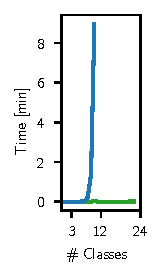
\includegraphics[height=0.5\columnwidth,trim={0 5pt 0 0},clip]{figures/plot_runtime.pdf}
    }
    \caption{SPP algorithms comparison over the UNSW dataset.}
    \label{fig:spp-example}
    \vspace{-16pt}
\end{figure}

Figure~\ref{fig:spp-example} provides a visualization of the accuracy-complexity trade-off of the greedy algorithm solving the SPP. We consider again the same inference task of Figure~\ref{fig:greedy}, but limiting it to a given number of classes, shown in the abscissa of the plots: when considering, \eg 9 classes, we randomly select 9 of the 24 classes that constitute the problem and run the greedy algorithm to identify a good partition of such 9 classes.
Figure~\ref{fig:gain-performance} shows that our proposed heuristic (green) performs substantially better than stochastic partitions (orange) with a gain that tends to increase as the complexity of the SPP grows.
The optimal solution (blue) clearly outperforms the greedy solution, yet Figure~\ref{fig:execution-time} shows that it also has an exponentially growing execution time that does not allow solving the SPP for more than a handful of classes. Instead, the greedy algorithm has a reasonable computational cost $O(m^2)$ in Figure~\ref{fig:execution-time}.

\subsection{Hardware-compliant ML sub-model training}
\label{sub:sub-models}

Stage \numO{4} trains one ML sub-model for each block in the partition $P^*$ output above. Unlike the unconstrained model trained in stage \numO{1}, these sub-models are designed to comply with the constraints of the target programmable network devices. Each sub-model aims at classifying the variables (\ie classes) present in the corresponding block, plus one additional \textit{others} category that gathers all classes that are part of the total inference problem but are not included in the current block.

Our implementation of \name relies on RFs to realize each ML sub-model. This choice is grounded in the significant success that RFs had as a reference ML paradigm for user-plane inference, as reported in Section~\ref{sec:related}.
The model design, hyper-parametrization and training are thus similar to those described in Section~\ref{sub:unconstrained-model} and rely on a joint packet- and flow-level inference model. The difference is that the bit representation of the features, the maximum number of trees, and the maximum number of leaves per tree are now constrained to abide by the limitations of user-plane hardware. Indeed, the limited size of register entries, the small amount of memory, and the finite number of stages in programmable devices force restrictions that must be accounted for at the design stage to ensure the compatibility of the ML models with the network equipment. Since we target a user plane composed of programmable switches, we adopt the techniques introduced in Flowrest~\cite{flowrest} to ($i$) engineer features and ($ii$) limit tree dimension, thus ensuring that the design of the ML sub-models is fully compatible with the network hardware.

The best RF sub-model for each block is identified from the grid search over the (constrained) hyper-parameters by balancing accuracy and resource usage. Specifically, we select the RF that maximizes
$\alpha\cdot \text{\sc{f1}} +(1-\alpha)\cdot \text{\sc{u\textsubscript{tcam}}}$, where \textsc{f1} is the \textit{macro F1} score defined in Section~\ref{sub:metrics}, \textsc{u\textsubscript{tcam}} is the expected usage of Ternary Content-Addressable Memory (TCAM) in the switch, and $\alpha$ is a tunable parameter that we set to $0.5$ in our experiments to fairly balance the two contributions.

\subsection{ML sub-model sequencing}
\label{sub:sequencing}

Stage \numO{5} orders the ML sub-models so as to optimize the inference performance. The sub-model sequencing impacts the distributed inference accuracy due to the following aspects.
\begin{itemize}
    \item Confusion between sub-models addressing different parts of the global inference. The problem arises due to false positives from an upstream sub-model that generates incorrect early decisions on flows that in fact belong to the target classes of downstream sub-models.
    \item Diverse accuracy of each sub-model. Sub-tasks have non-uniform complexity, and each sub-model has a different error rate that affects all downstream sub-models.
\end{itemize}
The goal of this stage is then to generate an ordering such that ML sub-models with a low rate of false positives and a high accuracy are deployed earlier in the sequence. \name solves a simple optimization problem to that end. The objective is
\begin{equation}
\min_{\pmb{X}} \sum_{i,j\in P^*\hspace*{-2pt},\;i\neq j} \; p_{ji} \cdot (1 - f'_{i}) \cdot x_{ij}, \quad x_{ij}\in\pmb{X}
\label{eq:seq-objective}
\end{equation}
where $p_{ij}$ is the rate of false positives%
\footnote{Since each ML sub-model is trained on the entire set of classes, it is possible to calculate the false positives across blocks. For instance, for the sub-model associated to block $S_i$ we can compute the rate of flows belonging to the classes in block $S_j$ that such a model misclassifies as its own.}
that the ML sub-model of block $S_i$ generates with respect to classes in block $S_j$ of the partition $P^*$, $f'_i$ is the \textit{macro F1} score of the sub-model for block $S_i$ trained in Stage \numO{3}, and $x_{ij}$ are binary decision variables that take value one if the ML-model of block $S_i$ precedes that of block $S_j$ in the ordering.

In order to ensure that each ML sub-model is executed only once in a valid order, we define the  following two constraints.
\begin{equation}
    x_{ij} + x_{ji} = 1, \quad \forall i,j \in P^*, i\neq j,
\label{eq:seq-objective_const1}
\end{equation}
\begin{equation}
    u_i - u_j + x_{ij} \cdot \|P^*\| \leq \|P^*\|-1 \quad \forall i,j \in P^*, i\neq j,
\label{eq:seq-objective_const2}
\end{equation}
where $u_i$ is an auxiliary variable associated with the block $S_i$ used to enforce the order of deployed sub-models and $\|P^*\|$ is the total number of blocks. The problem in~\eqref{eq:seq-objective}--\eqref{eq:seq-objective_const2} is a version of the well-known Travelling Salesman Problem and can be formulated as an ILP and solved efficiently.
%\da{I believe that the implementation is a version of the Travelling Salesman Problem. If so, it can be formulated as an ILP and solved with Gurobi (as Beyza did).}

\subsection{ML sub-model planning}
\label{sub:planner}

% The linear topology used in our hardware testbed deployment of \name does not capture the challenges of more complex network topologies, where multiple routing decisions and diverse network functionalities must be taken into account. 
% To address this, we deploy \name in an emulation environment featuring a range of complex topologies, demonstrating that \name can coexist with diverse routing decisions and network functions in more realistic network settings. 

The ordering returned by stage \numO{5} directly allows deploying the ML sub-models within a linear sequence of user-plane devices, so that the inference process can be distributed, \eg along a single, specific, predefined path.
However, routes in a real-world network are not independent sequences of disjoint sets of switches; they are instead intertwined paths resulting from traffic engineering decisions on underlying physical network topologies. A trivial solution is then deploying the complete sub-model sequence along all possible paths in the network, which would, however, cause an unnecessary duplication of functions, rapidly deplete the resources of switches, and ultimately not scale beyond tiny topologies.

To ensure that \name can be efficiently applied to real-world networks, stage \numO{6} determines the optimal deployment strategy for a given combination of network topology and routing, so that all flows forwarded through the target network are ensured to traverse all ML sub-models in the correct sequence. The goal is to guarantee such a condition while minimizing sub-model duplication across the network.
To this end, we devise a strategy inspired by the planner component of the DINC framework~\cite{dinc-conext23}, as follows.

For a given network topology and routing, the deployment strategy we develop aims to achieve two objectives: ($i$) minimize sub-model duplication across paths, and ($ii$) maintain the execution order of sub-models. To this end, we formulate an ILP with an objective function
\begin{equation}
\min \sum_{s\in S} \sum_{m\in M} \; X_{s \gets m},
\label{eq:dpl-str-objective}
\end{equation}
where $M := \{1, \dots, N_M\}$ is a linearly ordered set of sub-models obtained as explained in Section~\ref{sec:name-control-plane}, $S := \{1, \dots, N_S\}$ is a set of switches in a given topology, and $x_{s \leftarrow m}$ is a binary variable indicating whether sub-model $m$ is deployed on switch $s$, \ie $x_{s \leftarrow m}$ is $1$ if the sub-model $m$ is deployed on the switch $s$, $0$ otherwise. The objective minimizes the total number of sub-models deployed across the network. We then ensure that each sub-model is present at least once on every path by the following constraint
\begin{equation}
\quad \sum_{s \in P} X_{s \gets m} \geq 1
            \quad \forall m \in M, \forall P \in \mathcal{P},
\label{eq:model-coverage-constraint}
\end{equation}
where $\mathcal{P} := \{P_i\}_{i=1}^{N_p}$ is a set of paths in the given topology, and each path $P_i \in \mathcal{P}$ is an ordered sequence of switches.
Moreover, we need to guarantee the correct execution order of sub-models. For any two sub-models $m < m'$, if $m'$ is deployed on a switch at position $j$ along a path $P_i$, then $m$ must be deployed on a switch that appears earlier on the same path. Formally, this results in a constraint
\begin{equation}
 \quad \sum_{k=1}^{j-1} X_{s_i^k \gets m} \geq X_{s_i^j\gets m'}
            \quad \forall m < m',\forall i \in [N_p], \forall j \in [l_i],
\label{eq:dependency-constraint}
\end{equation}
where $l_i$ is the number of switches on the path $P_i$ and $s_i^k$ denotes the $k$-th switch on the path $P_i$ (\ie the $k$-th element of the sequence representing $P_i$).

The proposed ILP formulation in~\eqref{eq:dpl-str-objective}--\eqref{eq:dependency-constraint} can be resolved using a numerical solver; in our implementation, we used the PuLP~\cite{pulp} linear and mixed integer programming modeler.
%The network topology is represented as a graph, and all simple paths between host pairs are considered. Binary variables indicate sub-model deployments on switches, and the ILP is constructed accordingly with objective and constraint terms in ~\eqref{eq:dpl-str-objective}--\eqref{eq:dependency-constraint}. Once solved, the model-to-switch assignments are extracted to guide deployment decisions in our system.

\section{DUNE user-plane operation}
\label{sec:name-user-plane}

Upon completion of the training pipeline in Figure~\ref{fig:overview}, the ML sub-models are coded as P4 programs and deployed in the target programmable user plane, where the distributed inference is performed at line rate.
While the general framework we propose can be adapted to different user-plane configurations--potentially combining diverse types of programmable network devices--the implementation of \name in this paper focuses on networks of programmable switches.
We next present the new \name header used to encapsulate information necessary to the distributed inference process across switches in Section~\ref{sub:header}. We then illustrate the user-plane operation in a simple case in Section~\ref{sub:example} before discussing in Section~\ref{sub:processing_logic} the complete local processing logic that allows robust functioning of \name in real-world settings.

\subsection{DUNE header}
\label{sub:header}

\begin{figure}
    \footnotesize
    \centering
    \begin{bytefield}[bitheight=1.2\baselineskip]{32}
    \bitheader{0,15,31} \\
    \bitbox[tl]{16}{\texttt{EtherType}} & \bitbox{8}{\texttt{Level}} & \bitbox{8}{\texttt{Class}} \\
    \bitbox{8}{\texttt{Collision}} & \bitbox{8}{\texttt{ModelID}} & 
        \bitbox{16}[bgcolor=lightgray]{\texttt{PathID}} \\ %\textsuperscript{\ref{footnote:hdr}}} \\
    \end{bytefield}
    \caption{Structure of the \name header.
    % The path ID is used in the Mininet environment to route flows easily.
    For ease of implementation, all fields are padded to 8 bits. The \texttt{PathID} field is grayed to denote that it is only used in emulation environments to facilitate manual routing configurations.}
    \label{fig:dune_header}
\end{figure}


A distributed ML inference requires that dedicated state be propagated across switches participating in the process. We realize this by introducing a \name protocol header, organized as illustrated in Figure~\ref{fig:dune_header} and inserted between the Ethernet and IP headers of packets belonging to flows to be classified.

The \texttt{Level}, \texttt{Class}, \texttt{Collision}, and \texttt{ModelID} fields are used to exchange intermediate results between sub-models and to provide runtime feedback to the control plane.
Specifically, the \texttt{Level} field indicates whether the classification operates at the flow or packet level, while the \texttt{Class} field encodes the corresponding classification outcome.
The \texttt{Collision} field signals hash collisions by flagging packets whose flow identifiers have collided at any switch along the path.
Finally, the \texttt{ModelID} field ensures that sub-models are executed in the intended sequence.
The \texttt{EtherType} and \texttt{PathID} fields serve protocol and forwarding functions.
The \texttt{EtherType} field duplicates the value originally present in the Ethernet header, which is overwritten upon insertion of the \name header.
The \texttt{PathID} field enables MPLS-like forwarding across the network and is useful exclusively in emulated environments--such as the one we present in Section~\ref{sec:experimental-setup}--to easily route flows according to manually defined paths.

Inserting an additional header between the Ethernet and IP headers may lead to size constraints when the IP header occupies the entire payload space.
This limitation is not unique to our design, as other protocols—such as MPLS—encounter similar challenges.
However, the use of jumbo frames mitigates this issue by allowing Ethernet payloads to extend the standard MTU of 1,500 bytes, typically up to 9,000 bytes.

\subsection{Illustrative example of distributed inference}
\label{sub:example}

% Once the preparation of the ordered ML sub-models is complete, each RF can be coded as a P4 program and deployed in the target programmable user plane for distributed inference, as per stage \numO{6} in Figure~\ref{fig:overview}.
% While the general framework we propose can be adapted to different user-plane configurations potentially combining diverse types of programmable network devices, the implementation of \name we produce and test in this paper is intended for a network of programmable switches. 

\begin{figure}
    \centering
    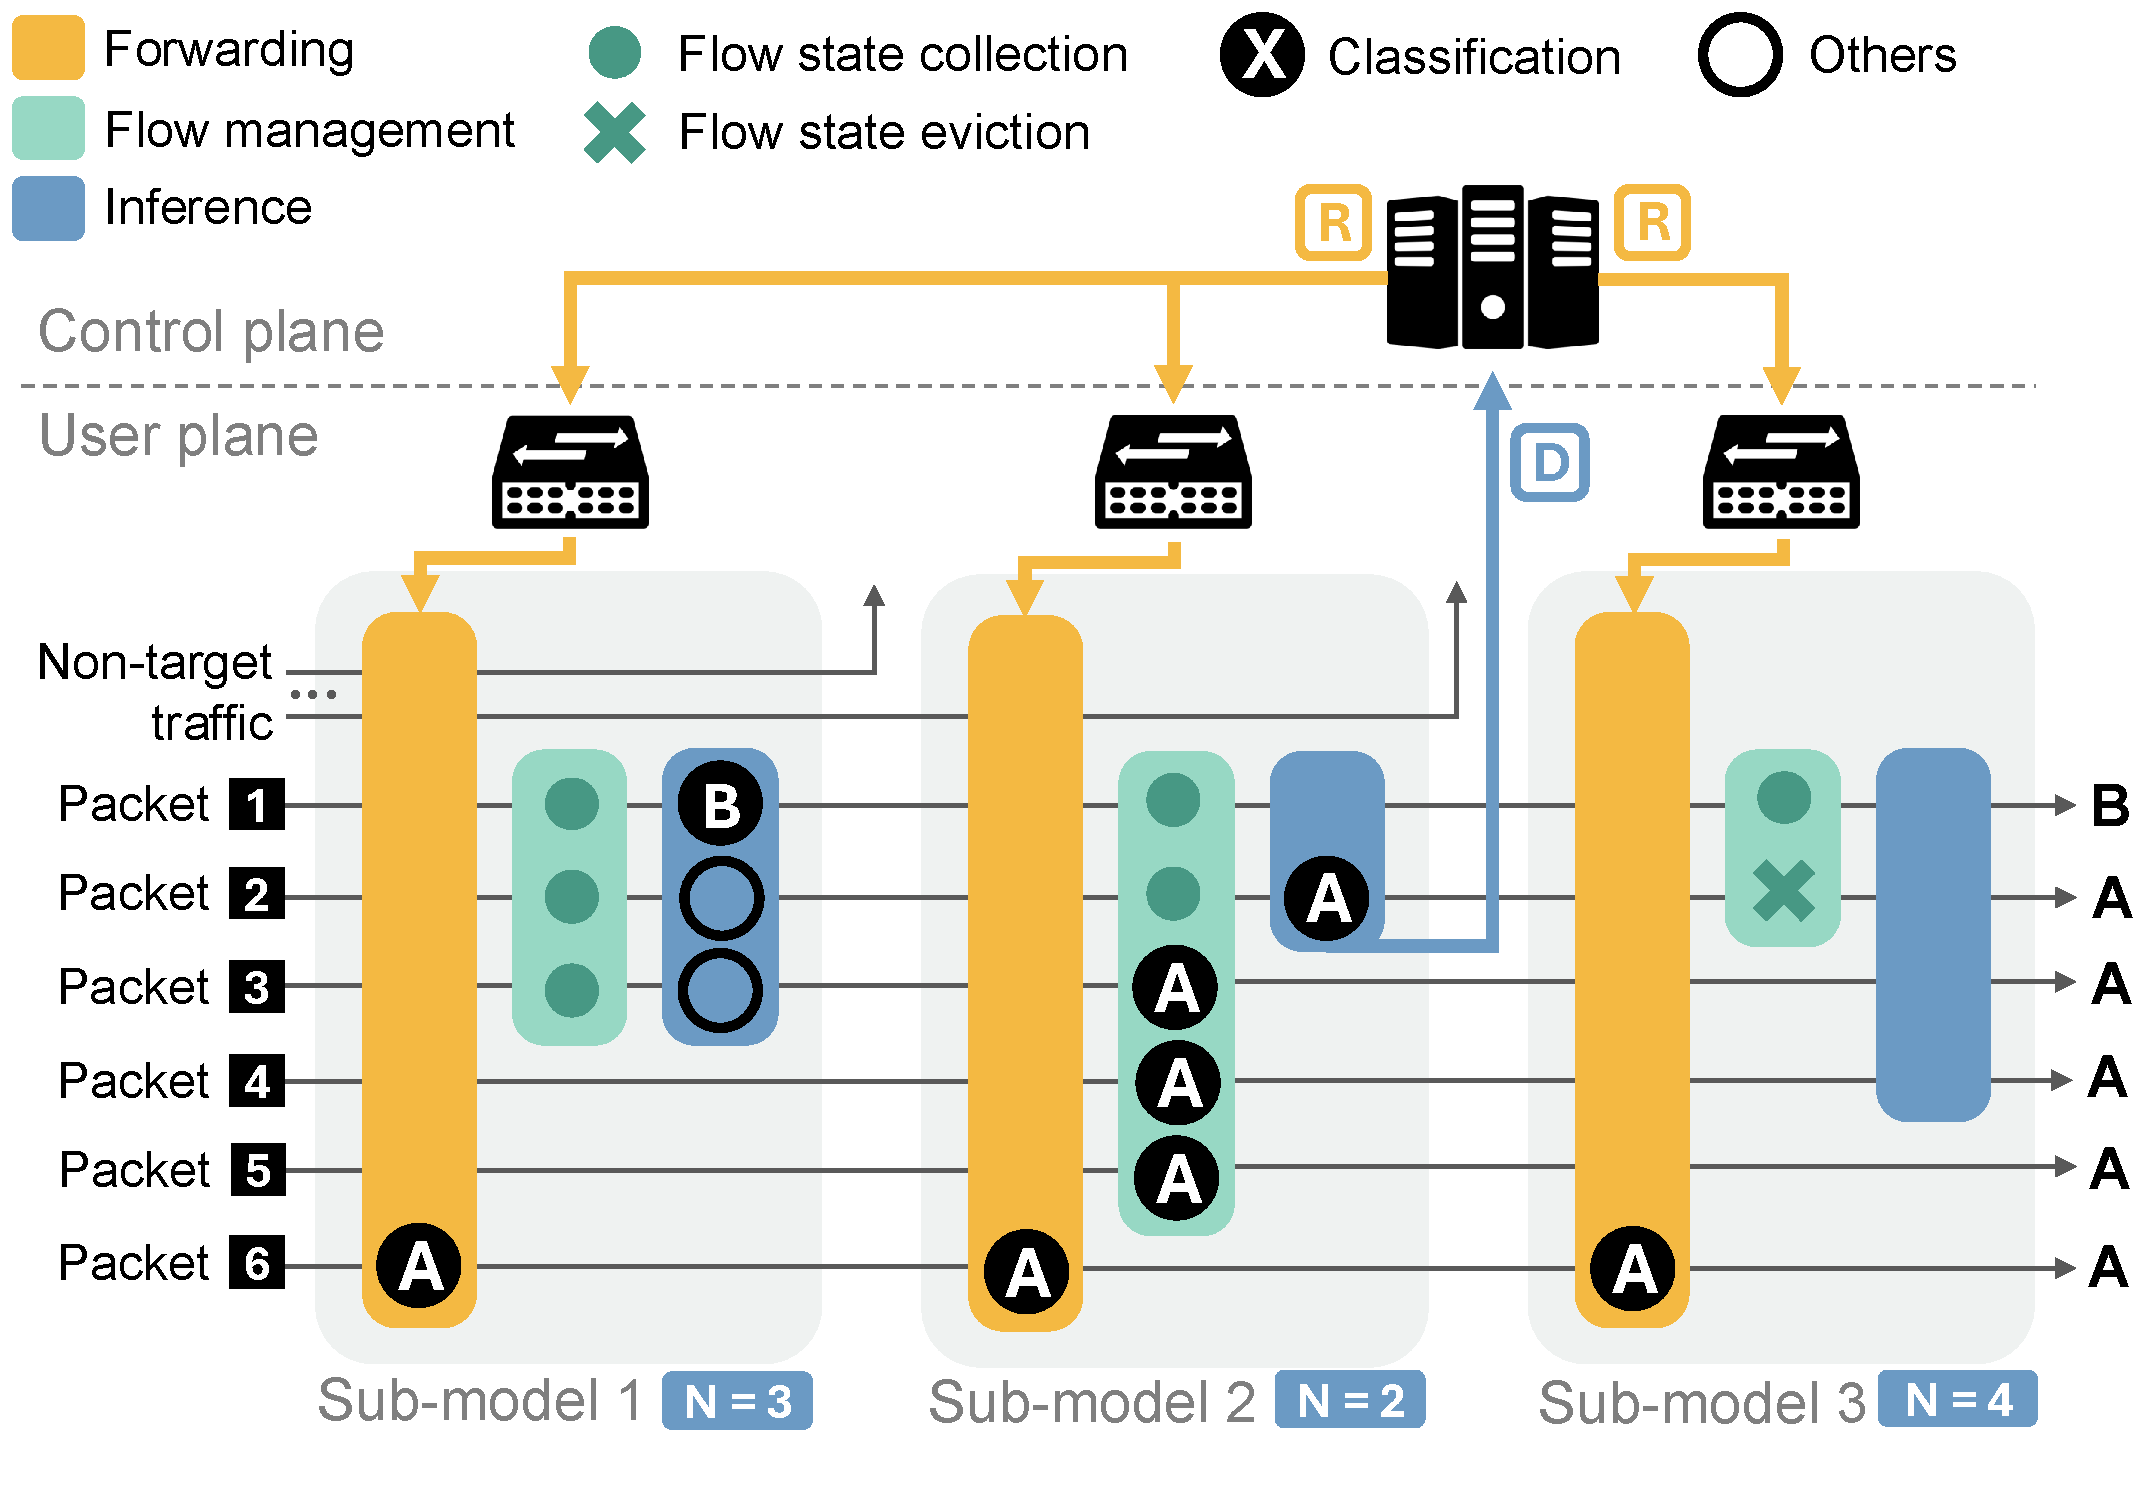
\includegraphics[width=\columnwidth]{figures/user-plane_updated.pdf}
    \caption{Simple example of the \name user plane operation with a distributed ML model over three switches performing inference on packets of one target flow.}
    \label{fig:user-plane}
    \vspace*{-16pt}
\end{figure}

The high-level operation of \name in the user plane is illustrated in a simple example in Figure~\ref{fig:user-plane}, where a sequence of three ML sub-models are deployed into three switches.
Each switch is programmed so as to perform three operations on a transiting packet: ($i$) \textit{forwarding} is the baseline function of the switch and consists in redirecting incoming traffic to its next hop or to the ML processing, depending on whether the flow is a target for inference or not; ($ii$) \textit{flow management} is only applied to flows for which inference needs to be run and stores stateful information about the flow-level features and situation (\eg classified or not) of every target flow;
($iii$) \textit{inference} is the actual Random Forest process that classifies a packet from the available input features.
%
We implement these three operations as in Jewel ~\cite{jewel-infocom24}. Importantly, this means that \name employs a single RF model to implement a joint packet- and flow-level approach in the inference component: the first packets of a flow are classified using features extracted from each individual packet only, whereas packets from the N-th leverage additional flow-level features collected from the first N packets of the same flow. Here, N is a configurable parameter that is determined during RF training~\cite{jewel-infocom24}.
% , and adopt the well-known Planter strategy~\cite{Planter.2021}
% to map RFs to P4 Match-Action Tables.
% to map efficiently RFs to the Match-Action Units (MAU) of each switch ASIC.

Once the network is programmed, the operation is as shown in Figure~\ref{fig:user-plane}. Traffic that is not a target for inference is normally forwarded by the switches according to their legacy forwarding tables. When the first packet of a flow that has to be classified is received by the entry switch (\eg packet 1 in the figure, whose flow we assume to belong to class A), it is forwarded to the local flow management stage, where flow-level information is collected and stored, and then moved to the inference stage. Since the first ML sub-model in this example performs flow-level inference on packet N=3, packet 1 of the flow is classified using packet-level features only, and in this specific example, is misclassified as belonging to class B. The packet is then moved along the distributed ML pipeline and traverses the two remaining switches: in both downstream switches, packet 1 is identified as a target for classification; hence, flow-level information is collected, but the packet skips the inference stage since it has already been tagged with a class, although incorrectly (\ie the \texttt{Class} field is set to `B').

When packet 2 arrives, it follows a similar path. However, let us assume that this time the packet-level inference run by the first switch does not tag packet 2 with a class but marks it as \textit{others}, \ie belonging to a class pertaining to a downstream ML sub-model as discussed in Section~\ref{sub:sub-models}.
Hence, packet 2 is forwarded to the second switch (with the \texttt{Class} field set to `others' and the \texttt{ModelID} field set to `1'), which updates its internal flow-level state with information from this packet. In the example, the second ML sub-model is, in fact, responsible for inferring packets and flow belonging to class A; also, the flow-level inference point in this model is N=2. The sub-model tags packet 2 as pertaining to class A and updates its local flow management to automatically associate all following packets for the same flow to class A.
Packet 2 is forwarded to the third switch, which lets it evict the associated flow-level data from the flow management registers since the flow has now been classified by an upstream switch (\ie the \texttt{Level}, \texttt{Class}, and \texttt{ModelID} fields in the packet received by the third switch are set to `flow', `A', and `2', respectively).

The classification of the flow also triggers a digest message D from the second switch to the control plane; this lets the centralized controller inject new forwarding rules R in all switches and release the flow-level registers. Once the control plane has injected the updated rules, the forwarding stages of all switches tag subsequent packets with their corresponding class and forward them accordingly. This is illustrated, \eg by packet 6, which is processed after the rule update.

% \da{Moved to implementation:}
% \textcolor{red}{\sout{It is worth noting that simple sub-models can be implemented in the same switch, in which case they share flow management registers and any common features.}}
%
% \footnote{The code repository will be provided after the double-blind review process.
% for full reproducibility of the solution and complete transparency of our \name user-plane implementation.


% \bb{How the implementation works in the switch - with the challenges that i mentioned and solutions (a brief explanation to make it clear):

% First switch (model) in the chain: It is not aware of the decisions taken in the downstream switches. Whenever a packet/flows comes, it runs the inference block if the packet count is less than or equal to the inference point. For the packets less than N, it tags them with the classification  result. If it is the flow classification, it tags them 'as classified' if the classification result is one of the classes, otherwise, it is tagged as 'unclassified'. This way, the downstream model can be aware of the FL classification and refresh the memory if the flow is classified.

% The switches in the middle/last: The first thing they do is to check if the incoming flow is classified. If it is classified, it sends a digest to refresh the memory with since there will be no incoming packets of this flow. 
% If the flow is not classified, it goes through all the flow-management process and if the packet is classified as 'Others' before, it runs the inference for that packet. Then, after tagging it according to the classification result, it forwards it.

% When i have problems in number of stages, i have changed some parts of the implementation and made it simpler. Everything works the same but with some small tricks. 
% 1) When I exceeded the available number of stages in the middle switches, I skipped the classified tag that it set when FL classification happens (so that the downstream models can refresh the memory). In this case, the consecutive switch checked the pkt count of this packet and classification result. Then, it decided if this packet is the Nth and classified as one of the classe or not (send a digest to refresh memory accordingly). This is not related to implementing two models into the switch. It will be in (2).

% 2) This is something i always did whenever i deployed 2 models into one switch. After the flow management, if the packet count less than N (which is the biggest N value of 2 models), it always executes the inference of two models even if the first model in the same switch decides that this packet belongs to one of the classes.
% It means it first execute 2 inference, then checks the results. If the first one already classifies the packet, the packet is tagged with this class. Otherwise, it takes the decision of the second model.
% }

\subsection{Switch local processing logic}
\label{sub:processing_logic}

\begin{figure}
    \centering
    \begin{adjustbox}{width=\columnwidth}
        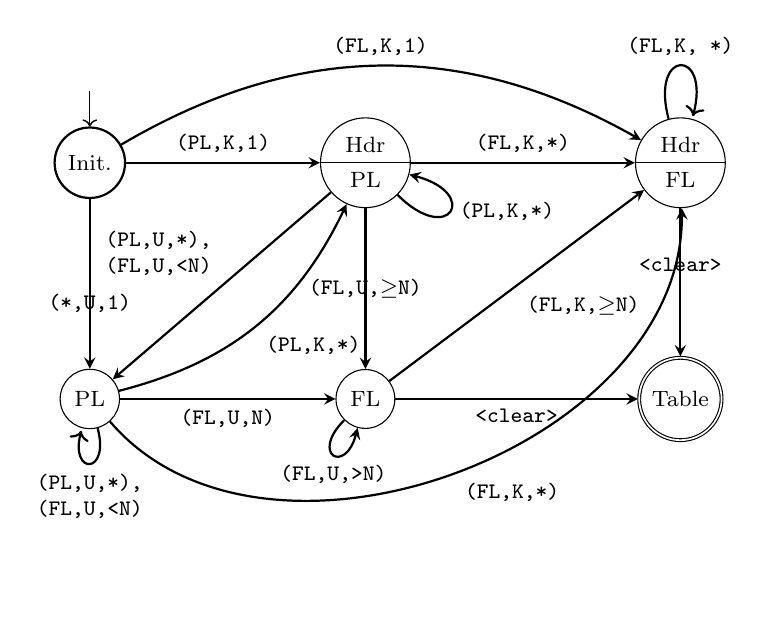
\begin{tikzpicture}
            % Help lines :
            % \draw [help lines] (-1,1) grid (9,-5);

            % States
            \node (init) [
                state,
                initial,
                % ultra thick,
                thick,
                initial above,
                initial text={},
            ] at (0,0) {Init.};
            \node (hdrPL) [
                state with output,
            ] at (3.5,0) {Hdr \nodepart{lower} PL};
            \node (hdrFL) [
                state with output,
            ] at (7.5,0) {Hdr \nodepart{lower} FL};
            \node (pl) [
                state,
            ] at (0,-3) {PL};
            \node (fl) [
                state,
            ] at (3.5,-3) {FL};
            \node (table) [
                state,
                accepting,
            ] at (7.5,-3) {Table};

            % Edges
            \path [-stealth, thick]
                % Out of init
                (init) edge node [above] {\texttt{(PL,K,1)}} (hdrPL)
                (init) edge [bend left=30] node [above] {\texttt{(FL,K,1)}} (hdrFL)
                (init) edge node [below] {\texttt{(*,U,1)}} (pl)

                % Out of hdrPL
                (hdrPL) edge[out=315, in=345, looseness=8] node[right] {\texttt{(PL,K,*)}} (hdrPL)
                (hdrPL) edge node [above] {\texttt{(FL,K,*)}} (hdrFL)
                (hdrPL) edge [] node [above left,align=center] {\texttt{(PL,U,*),}\\ \texttt{(FL,U,<N)}} (pl)
                (hdrPL) edge node [] {\texttt{(FL,U,$\ge$N)}} (fl)

                % Out of hdrFL
                (hdrFL) edge [loop above] node [above] {\texttt{(FL,K, *)}}()
                (hdrFL) edge node [above] {\texttt{<clear>}} (table)

                % Out of PL
                (pl) edge [loop below] node [below,align=center] {\texttt{(PL,U,*),}\\ \texttt{(FL,U,<N)}}()
                (pl) edge [bend right=25] node [below right] {\texttt{(PL,K,*)}} (hdrPL)
                (pl) edge [bend right=70] node [below right] {\texttt{(FL,K,*)}} (hdrFL)
                (pl) edge node [below] {\texttt{(FL,U,N)}} (fl)

                % Out of FL
                % (fl) edge [loop below] node [below] {$(FL,U,>n)$}()
                (fl) edge[out=225, in=255, looseness=8] node [below] {\texttt{(FL,U,>N)}}(fl)
                (fl) edge [] node [below right] {\texttt{(FL,K,$\ge$N)}} (hdrFL)
                (fl) edge node [below] {\texttt{<clear>}} (table)
            ;
        \end{tikzpicture}
    \end{adjustbox}
    \vspace{-2\baselineskip}
    \caption{State machine for the local processing logic for one traffic flow at a switch. States indicate the action taken by the switch on incoming packets, whereas edges represent state transitions triggered by the reception of packets with specific \name header information.}
\label{fig:state_machine}

\end{figure}

The simple example in Section~\ref{sub:example} illustrates the operation of \name in a straightforward linear network topology under ideal settings. In practice, the distributed inference process has to operate in real-world, complex networks where packet reordering and loss can occur, which creates a variety of corner cases whose management requires a careful and robust user-plane implementation.

To ensure that \name correctly operates in all possible scenarios that may happen in realistic user planes, we design a state machine that tracks the provenance of classification results within each switch. This state machine governs how incoming packets are interpreted based on the data carried in the packet headers from upstream switches. It thus defines the logical pipeline executed inside the switch to determine whether an inference result needs to be produced locally or if only propagation to downstream switches is instead required.

Figure~\ref{fig:state_machine} illustrates the states and their associated transitions.
Each state corresponds to an action executed by the switch. State transitions are triggered by three inputs: ($i$) the classification type, ($ii$) the result status, and ($iii$) the flow packet count.
% \mf{There is no packet count in the header in Figure~\ref{fig:dune_header}, should we add it or is the count a switch-local state only?}
Specifically, the classification type is either \texttt{PL} (packet-level) or \texttt{FL} (flow-level), indicating whether the classification was performed at the packet or flow level in upstream switches and extracted from the \texttt{Level} field of the \name header. The result status is denoted as \texttt{U} (Unknown) or \texttt{K} (Known), where a result is considered Known if it matches one of the predefined classes in the dataset, and Unknown if it is classified as \textit{others}, as observed in the \texttt{Class} field of the \name header. The last input, \ie the packet count in the flow, is maintained locally by the switch as part of the \name flow management routine.

The state machine begins in the \texttt{Init} state, where no classification has yet been performed. Upon receiving an incoming packet, the switch evaluates its classification type, result status, and packet count to determine the appropriate transition. 
If the first packet of a flow is classified as \texttt{FL-K} in one of the upstream switches, the current switch bypasses inference and simply propagates the result to downstream switches, while also sending a digest to the controller to refresh the memory associated with the flow and to update the forwarding table accordingly. The switch remains in the same state of \texttt{Hdr/FL} for all subsequent packets belonging to the same flow.
If the first packet of a flow arrives with \texttt{PL-K} from upstream switches, it transitions to the \texttt{Hdr/PL} state and propagates the packet-level result. It continues to propagate packet‑level results—and stay in that state—as long as each new packet is again classified as \texttt{PL-K} by an upstream model. Even if the packet count is equal to the inference point N, the switch does not run FL inference and waits for the FL inference result from the upstream switches, as per the following Assumption~\ref{ass:model_order}.

\begin{assumption}
  The ML sub-models \(m_1<\dotsb<m_n\) are ordered from best to worst according to the model sequencing stage \numO{5} described in Section~\ref{sub:sequencing}.
  Hence, for any two models \(m_i<m_j\), the output produced by \(m_i\) is more accurate than that produced by \(m_j\), when applied to the same input.
  \label{ass:model_order}
\end{assumption}

While the switch is in the \texttt{Hdr/PL} state, the arrival of a packet with \texttt{FL-K} (\ie with a class determined by a flow-level inference in an upstream switch) triggers a system transition to the next state, \texttt{Hdr/FL}, where the switch propagates the FL decision and sends a digest. If instead a packet arrives with a classification of \texttt{FL-U} and the observed packet count is greater than or equal to the inference point, the switch moves from the \texttt{Hdr/PL} state to the \texttt{FL} state, where local flow-level inference is executed. The switch sends a digest to clear its registers and update tables accordingly upon classifying the flow as Known, as in the following Assumption~\ref{ass:local_FL_K}.

\begin{assumption}
  If the local result is \texttt{FL-K}, we initiate the process to populate tables accordingly and clear registers of the switches
        on the path of the flow.
    \label{ass:local_FL_K}
\end{assumption}

Given a switch in the \texttt{Hdr/PL} state for the target flow, the reception of a packet with \texttt{PL-U} or \texttt{FL-U} and a packet count less than the inference point lets the switch transition to the \texttt{PL} state, where local PL inference runs. A transition to this state also happens when a switch in the \texttt{Init} state receives a packet with any Unknown classification result. So, the switch transitions to this state only if there is an Unknown classification result due to the following Assumption~\ref{ass:packet_order}, which forms the basis for Assertion~\ref{assr:pl_state} and Assertion~\ref{assr:fl_inference} below.

\begin{assumption}
    A flow of packets goes through models following the order
        provided by model sequencing.
        \label{ass:packet_order}
\end{assumption}

\begin{assertion}
A result of type \texttt{PL} can only be produced locally if it was previously classified as \texttt{PL-U} or \texttt{FL-U}.
\label{assr:pl_state}
\end{assertion}

\begin{assertion}
A result of type \texttt{FL} can only be produced locally if it was previously classified as \texttt{FL-U}.
\label{assr:fl_inference}
\end{assertion}

The switch transitions from the \texttt{PL} state to the \texttt{Hdr/FL} state upon receiving a packet with \texttt{FL-K}. If it receives a packet with \texttt{PL-K}, it transitions again to the \texttt{Hdr/PL} state to propagate the packet-level classification results obtained by upstream models. It stays in the same state, \texttt{PL}, where it runs PL inference locally, as long as it receives packets with \texttt{PL-U} (due to Assumption~\ref{ass:model_order}) or \texttt{FL-U} with a packet count less than the inference point. Whenever the switch receives a packet with \texttt{FL-U} at the inference point, it transitions to the \texttt{FL} state to classify the flow and propagate the local result to the downstream switches.

Finally, the switch remains in the \texttt{FL} state unless it receives a packet with \texttt{FL-K}. In that case, it proceeds to \texttt{Hdr/FL} to directly propagate the result to the downstream switches.

\section{Implementation}
\label{sec:implementation}

We implemented \name on both software and hardware P4 targets. The former allows exploring the operation of the framework on complex topologies and at scale, whereas the latter lets us validate its viability with limited topologies but real-world production-grade devices. Due to fundamental differences in the target architectures, the two implementations vary in terms of restrictions and performance, as detailed next.

\subsection{bmv2 software target}
\label{sub:software}

Our software implementation is written for the v1model architecture and runs on the \texttt{simple\_switch\_grpc} target~\cite{simple_switch}, which is based on the bmv2 framework~\cite{bmv2}.
This software switch offers high flexibility--virtually infinite resources only bounded by the servers where the emulation runs--but low performance, \ie it is intended for testing, prototyping, and research, but not production scenarios with moderate to high throughput.
However, its nature makes it possible and affordable to spawn many software instances and compose large arbitrary topologies.
%As Intel discontinued the production of Tofino ASICs,
Moreover, given the cost of hardware switches and the recently discontinued production of Tofino ASICs, this software implementation is particularly valuable in making \name accessible to the community at large.

Unfortunately, the limited performance of bmv2 also brings functional limitations.
For instance, using time-based features for inference in a bmv2 implementation is impractical, since such features depend on high-precision timing when recording packet arrival times, which the software cannot guarantee.
The non-deterministic packet processing time of bmv2 can also curb stateful processing, since it introduces variability at runtime with concurrent flows that might, or might not, contend for resources.
In addition, bmv2 also has significant shortcomings when it comes to interfacing with control plane agents.
On the one hand, its legacy Thrift-based interface does not support the digest mechanism, which is critical to request table insertions.
On the other hand, the current gRPC-based interface, while supporting digests, does not support the manipulation of registers, key for evicting classified flows.
More challenges come from the library used by bmv2 to interface over gRPC, \ie \textit{P4Runtime-Shell}, which makes use of global variables and precludes the establishment of parallel connections from the same agent, de facto forcing us to handcraft the gRPC messages instead.

As a workaround to all these issues, our control-plane design is multi-threaded, with each thread dedicated to a single device and holding one gRPC and Thrift connection.
This lets us correctly implement a central controller connected to all the devices running \name ML sub-models, which, in line with the user-plane operation presented in Section~\ref{sec:name-user-plane}, yields two important practical benefits upon classification of a flow: ($i$) the controller can populate table entries in all devices, significantly reducing the time-to-classification when results are obtained at downstream models; and ($ii$) the controller can free registers selectively, avoiding the eviction of flows with colliding register indices.
This is particularly relevant in multi-path network topologies, where diverse flows mapped to the same register index can have their state stored at different switches--hence a global eviction at all switches based on the index would result in the deletion of erroneous flows.

\begin{figure}
    \centering
    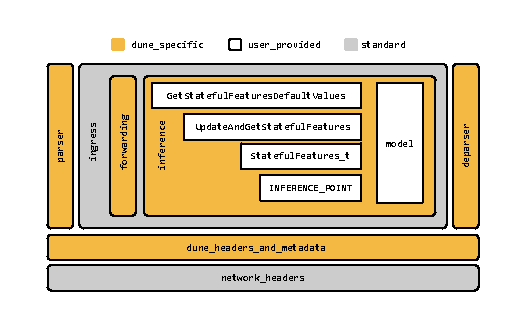
\includegraphics[trim={0 0.5cm 0 0.65cm},clip]{figures/code_arch.drawio.pdf}
    \caption{\name software implementation blocks, separating elements that are part of the standard bmv2 emulator, specific to our \name implementation, or expected to be provided by the end user in order to run a specific inference task. }
    \label{fig:code_arch}
    \vspace{-13pt}
\end{figure}

Finally, it is worth remarking that our \name implementation is modular and only requires users to input a few model-dependent blocks and variables before running the framework. As illustrated in Figure~\ref{fig:code_arch}, users shall provide: (1) the \texttt{\footnotesize StatefulFeatures\_t} type, encapsulating the set of required stateful features; (2) the \texttt{\footnotesize UpdateAndGetStatefulFeatures} and \texttt{\footnotesize GetStatefulFeaturesDefaultValues} control blocks, encapsulating the update logic and default values for the provided stateful features, respectively; (3) the \texttt{\footnotesize INFERENCE\_POINT} constant indicating the number of packets used for feature computation; and, (4) the \texttt{\footnotesize InferenceModel} block encoding the trained RF as a set of feature and code tables~\cite{ilsy-hotnets19}.

\subsection{Intel Tofino hardware target}
\label{sub:hardware}

\begin{table}[t]
\centering
\caption{Comparison of v1model (bmv2) and TNA (Tofino1) architectures, across five dimensions (rows).}
\label{tab:v1model_vs_tna}
\begin{tabular}{@{} l p{2.8cm} p{4.1cm} @{}}
\toprule
\textbf{Dimension} & \textbf{v1model} & \textbf{TNA} \\
\midrule
\multirow[t]{2}{*}{Pipeline} & parser → ingress → & parser → multi-stage ingress →\\
 & egress → deparser → & traffic manager → multi-stage egress → deparser \\ \midrule
\multirow[t]{2}{*}{Resources} & Abstract, unlimited & Hardware-constrained \\
& & (\eg stages, SRAM/TCAM, ALUs) \\ \midrule
\multirow[t]{2}{*}{Externs} & Counters, meters, & Tables, selectors, multicast,\\
&  registers, clone/resubmit & queueing, PRE, hashing \\ \midrule
% Metadata & Minimal: ports, length, type & Detailed: ports, queues, timestamps, replication, drop reasons \\
\multirow[t]{2}{*}{Limitations} & non-deterministic performance;& Stage/table limits; unsupported operations\\
& timing precision & (\eg unbounded tables, arbitrary recirculation, arbitrary packet modifications) \\ \midrule
Use case & Prototyping \& education & High-performance deployment \\
\bottomrule
\end{tabular}
\vspace{-8pt}
\end{table}

Our hardware implementation of \name is coded for the Tofino Native Architecture (TNA) and targets the Tofino 1 chipset.
%
Unlike the v1model architecture, which offers conceptually infinite resources, the TNA exposes a realistic and constrained pipeline.
Table \ref{tab:v1model_vs_tna} summarizes the differences between the v1model and TNA across several dimensions. This lets us highlight the most challenging constraints of a hardware implementation: ($i$) table sizes, stage placement, and match types are fixed; ($ii$) stateful actions must respect atomicity per stage, limiting concurrency; ($iii$) arbitrary packet header manipulations or timestamp-based logic are hardware-limited, \eg divisions are not supported.
However, once successfully compiled, TNA-based programs offer strict guarantees on line-rate throughput and deterministic processing time.

Owing to the limitations above, model implementations are case-specific for the Tofino targets, often requiring careful code engineering and refactoring to fit the P4 program in the ASIC.
Consequently, providing a user-friendly \name framework equivalent to the software one is extremely challenging in the presence of real-world hardware.
While we engineered the software implementation to be amicable to hardware--\eg avoiding unsupported operations such as divisions, ensuring a single per-packet access per register, and using standard-length words at 8, 16, or 32 bits--ensuring that ML sub-models fit the ASIC stages (\eg 12 in the case of Tofino 1) is a non-trivial task left to the end users.
%Since our testbed comprises 3 devices, we are constrained in the number of models to those we can fit to their resources.

Specifically, the \name implementations we use in our experimental validation employ the efficient Planter mapping of sub-model RFs to the Match-Action Units (MAU) of the Tofino 1~\cite{Planter.2021}.
% With careful design, this mapping lets us implement multiple models in a single compilable P4 program running at an individual switch, by sharing flow management registers and common feature state.
With careful design, this mapping lets multiple models run on the same switch within a single P4 program, sharing flow management registers and common feature state.
The co-location of ML sub-models within the same switch 
inherently increases the consumption of SRAM and TCAM needed to encode the different RFs; however, it does not necessarily increase the number of consumed stages, since the tables of different sub-models can be evaluated in parallel and hence compiled into the same MAUs.
This is an important observation, as stage consumption is the most severe constraint of the target hardware and stays primarily determined by the number of dependent operations in the critical path of the pipeline within each RF.
%We consumed X, Y, and Z stages of each device, respectively, to implement the 3 UNSW-related models, and A, B, and C stages to implement the 4 ToN-IoT-related models, respectively. \bb{Please provide the number of consumed stages.}\\

As far as the control plane is concerned, our \name controller binds to the switches using the Barefoot Runtime Interface (BRI) and performs the initial setup of the switch: activating the ports and loading the trained ML models as table entries in the corresponding P4 tables.
During inference, the control plane collects the digest messages that include classification results and, based on such information, updates registers and tables in the user plane at run time.
We remark that control-plane-related issues in hardware are also different from those in the software implementation.
For instance, the line rate processing of the Tofino can result in digest message bursts if the replayed traffic is bursty; indeed, such messages are transmitted over the Linux IP stack and, thus, are subject to drops upon congestion, hindering results collection.
The alternative of capturing egress traffic is equivalently challenging for the same reason.
Thus, we still adopt the digest approach, which, in our experiments, results in a negligible 0.83\% of non-tracked flows due to digest loss.

\section{Experimental setup}
\label{sec:experimental-setup}

% \td{Combine subsection A and B and explain them together (Hardware and Software environment). Have another subsection to explain Linear and Clos topologies. You can also explain how we inject and collect the traffic here in this subsection.}

We test the hardware and software implementations of \name in relevant emulation and experimental environments (Section~\ref{sub:testbed}) reproducing simple linear and real-world fat tree network topologies (Section~\ref{sub:topologies}). Across these configurations, we deploy \name to solve challenging inference tasks (Section~\ref{sub:use-cases}) and evaluate its performance via sensible performance metrics (Section~\ref{sub:metrics}), comparing it against four state-of-the-art benchmarks (Section~\ref{sub:benchmarks}).

\subsection{Emulation and experimental environments}
\label{sub:testbed}

We evaluate the hardware implementation of \name in an experimental testbed that comprises $2$ servers and $3$ programmable switches operating as a comprehensive 100-Gbps platform.
The servers are equipped with AMD EPYC 24-core processors running at 2.8 GHz, with 128 GB of RAM, and QSFP28 interfaces.
The switches are production-grade Edgecore Wedge 100BF-QS programmable switches, featuring Intel Tofino BFN-T10-032Q chipsets and 32 100GbE QSFP28 ports.
All switches run the Open Network Linux (ONL) on top of Debian GNU/Linux 10 (Buster) as the operating system, and use the Intel Software Development Environment (SDE) version 9.13.2 for compiling P4 programs.
In the experiments, we distribute the inference process across the switches using \name, with one server dedicated to implementing the control plane; the other server is used to inject traffic in the network.
% {\color{blue}
% n the one hand, it injects measurement data from the classification use cases presented next, by replaying \var{pcap} traces using Tcpreplay~\cite{tcpreplay}. On the other hand, it employs the MoonGen packet generator~\cite{MoonGen} to inject background traffic at 100~Gbps, simultaneously to the use case traffic.
% This background traffic is not a target for inference, hence it is advanced by the traffic filtering module in Figure~\ref{fig:solution_hl} to the regular forwarding table of the switch. The rationale for having it is to demonstrate that the tested models can achieve line-rate inference even in presence of substantial concurrent non-target traffic.}
The results of inference experiments in the experimental platform are retrieved via digests, which convey the inference outputs to the control plane.

The emulation environment employed to test the software version of \name builds on Mininet \cite{team2017mininet}. Specifically, we employ the \texttt{simple\_switch} software target for the nodes, which are deployed on a server with 2.8 GHz AMD EPYC 24-core processors and 128 GB of RAM. The setup allows emulating large networks composed of hundreds of switches and injecting real-world traffic into those systems.
To collect experimental results in emulation, we process the output PCAP files generated by the \texttt{simple\_switch} at egress switches. Using \texttt{tshark},we extract both the packet five-tuple and the \name header, which carries the classification result and the information about collision.

\subsection{Network topologies}
\label{sub:topologies}

We use \name to distribute the inference process in two types of networks, each with a specific purpose, as detailed next.

\noindent \textbf{Linear topology.}
This is a simple network consisting of a sequence of switches connected to form a chain, where each switch forwards traffic to the next one until the destination is reached. Hosts are attached to the edge switches at either end of the chain. In this setup, the host connected to one edge switch acts as the source host, generating traffic, while the host at the opposite end acts as the sink host, receiving traffic, so that all traffic must traverse the entire chain of switches.
In this topology, we replay input traces from the source host toward the sink one, where the results are collected; the linear structure ensures that collisions are limited to those originated by simultaneous flows with identical hashes.

Ultimately, this topology is utilized for feasibility experiments to ($i$) demonstrate the practical viability of \name in our experimental platform, where the limited number of switches does not allow more complex network configurations, as well as ($ii$) validate the consistency of our software and hardware \name implementations in an uncomplicated scenario.

\begin{figure}
    \centering
    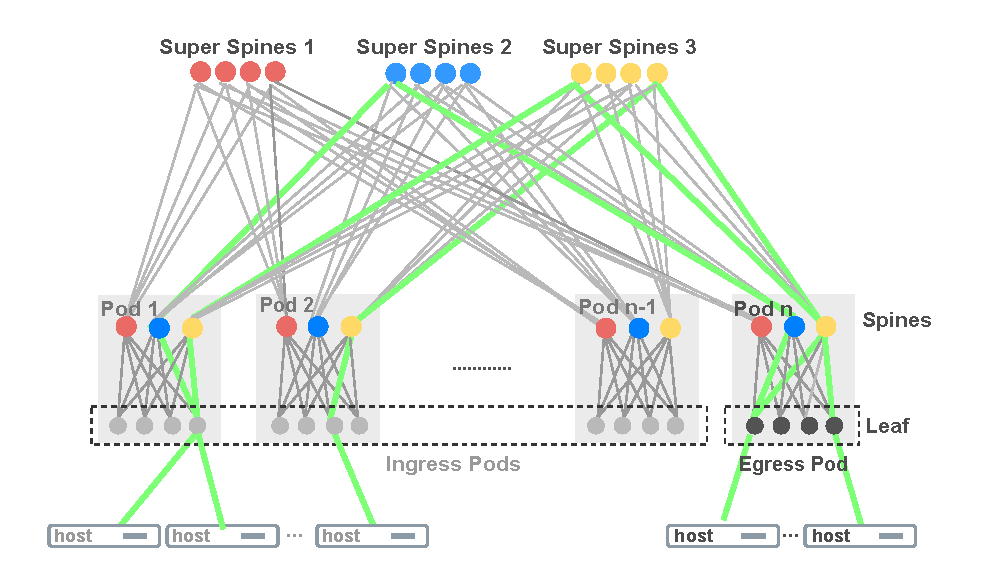
\includegraphics[width=\columnwidth]{figures/topology.pdf}
    \caption{Fat Tree topology considered in our experiments.}
    \label{fig:clos_topology}
    \vspace*{-8pt}
\end{figure}

\noindent \textbf{Fat Tree Topology.} This topology is a specific instance of the Clos topology, which is widely used in modern data centers for its scalability and high bandwidth. Figure~\ref{fig:clos_topology} illustrates our reference architecture based on a Fat Tree topology, inspired by large-scale real-world networks. Its design consists of three hierarchical layers: a leaf layer at the bottom, a spine layer in the middle, and a super spine layer at the top.
Leaf and spine switches are organized in pods, where leaf switches connect to hosts and forward traffic to spine switches within the same pod. The spine switches, in turn, connect upward to multiple spine planes, each consisting of a group of super spine switches. In the visualization of Figure~\ref{fig:clos_topology}, spines with the same color belong to the same spine plane, emphasizing the logical grouping and parallelism in the topology. This structure enables multiple parallel, equal-cost paths between any pair of ingress and egress pods.
The green paths highlight an example data flow from multiple ingress pods to a single egress pod. Specifically, they illustrate how traffic from different source pods is routed upward through their local spine switches, distributed across different spine planes, and then routed downward into the spine and leaf switches of the destination pod: this mimics a North-South communication within a data center where the egress pod provides external communication. 

In our experiments, we inject traffic from all hosts attached to the leaf switches of ingress pods, thereby distributing the load across pods and paths.
The traffic is directed toward hosts connected to the leaf switches of the egress pod.
For this purpose, we split the input PCAP trace into as many subsets as there are hosts, assigning one subset to each ingress host.
The splitting is performed at the flow level, ensuring that the number of flows is evenly distributed across hosts%
\footnote{Note that this traffic assignment does not guarantee traffic balance across hosts, as flows might have varying throughput and duration.}.
As a consequence of the funneling caused by the north-south communication, flow collisions in the Fat Tree topology increase substantially compared with the linear topology.
%Replaying flows in parallel results ini artificial collisions that do not exist originally, \eg the flow arrival time between colliding flows is longer than the time to classify the first flow.

We employ the Fat Tree topology to evaluate \name at scale in a realistic network, using our emulation environment. 
These tests also let us assess the impact of complex multi-path routing and its associated collisions on the operation of distributed inference.
\vspace{-8pt}
\subsection{Inference use cases}
\label{sub:use-cases}

We select two complex classification tasks in device identification and attack detection that are based on publicly available real-world measurement data to show how \name performs across different and demanding use cases.

\textbf{UNSW-IoT}~\cite{unsw_IoT_traces} is a device identification use case based on traffic measurement data collected from $26$ Internet of Things (IoT) and several non-IoT devices. Measurements are conducted in a living lab emulating a smart environment over a period of $6$ months. In order to detect which of the $26$ devices that traffic flows belong to, we train ML models with $15$ days of data and test with one day of data.


\textbf{ToN-IoT}~\cite{ToN_IoT_Telemetry_dataset} is an attack detection use case where benign, and $9$ types of cyberattacks are generated within a representative medium-scale testbed. This testbed comprises several IoT and industrial IoT (IIoT) devices, along with various non-IoT devices. 
% It also incorporates several virtual machines, including hosts running Linux and Kali Linux operating systems, to manage the interconnections across the Cloud, Fog, and Edge network domains. 
For our analysis, we use $75\%$ of the data for training and the remaining $25\%$ for testing. While the dataset contains benign traffic and nine types of cyberattacks, three of the latter are excluded from our analysis since they have insufficient samples in the test set. This results in the final task of categorizing traffic into seven classes.

\subsection{Inference accuracy metrics}
\label{sub:metrics}

We assess the performance of \name and of the selected benchmarks using the F1 score commonly used for evaluating classification accuracy. This metric is calculated based on three key measures: true positives (\textsc{tp}), false positives (\textsc{fp}), and false negatives (\textsc{fn})
as \textsc{f1}=100$\times$2\textsc{tp}/(2\textsc{tp}+\textsc{fp}+\textsc{fn}). We compute the F1 score by averaging the user-plane classification results with three different methods: ($i$) \textit{micro} average, which sums the \textsc{TP}, \textsc{FP}, and \textsc{FN} across all classes before calculating the metric; ($ii$) \textit{macro} average, which is the mean of the F1 scores of each class; and ($iii$) \textit{weighted} average, which weights the F1 scores of each class by the number of samples in the dataset.
%The benchmark solutions are evaluated using F1 score metric but with a different approach in their original paper. The packet-level solution Mousika and hybrid solutions NetBeacon and Jewel are evaluated packet-basis while the performance score is calculated flow-basis in flow-level solution Flowrest.
For a fair assessment of the performance of the different models, we use a \textit{flow-level} metric that operates on packets but removes the bias caused by long flows~\cite{flow-level-metric}: the score is calculated with packet-level \textsc{tp}, \textsc{fp}, and \textsc{fn} where each packet has a weight $w = 1/l$, being $l$ the length of the flow the packet belongs to.

\subsection{Benchmarks}
\label{sub:benchmarks}
We benchmark \name against four state-of-the-art in-switch classification solutions: Mousika~\cite{mousika-journal-ton23}, Flowrest~\cite{flowrest}, Netbeacon~\cite{netbeacon}, and Jewel~\cite{jewel-infocom24}. All use monolithic ML models.

\textbf{Mousika} is a packet-level (PL) classifier leveraging knowledge distillation.
In this approach, a Random Forest (RF) or Decision Tree (DT) is trained and distilled into a single Binarized Decision Tree (BDT).
We implement Mousika using the publicly available source code~\cite{code-mousika} and
use our model analysis approach to run a grid search over the hyperparameters and PL features, which are later binarized and used to train the teacher RF or DT model.
As the BDT student model uses a compact binary-tree representation, we need not limit its size.

\textbf{Flowrest} is a resource-aware, tree-based solution for flow-level (FL) inference. Thanks to its flow management strategy, it allows tracking and classifying flows directly in the data plane.
Yet, during the flow feature collection phase, it is unable to classify packets; thus, it is not suitable for classifying traffic with predominantly short-lived flows.
The Flowrest instance we use is based on the available source code~\cite{code-flowrest}.

\textbf{Netbeacon} is a tree-based solution capable of performing PL classification for short flows and FL classification otherwise.
To this end, Netbeacon deploys 3 sets of models: an XGBoost model to predict flow sizes; a PL classifier for short flows, collided flows, and pre-FL-inference packets;  and FL classifiers with variable inference points---depending on the flow length--- to classify long flows.
Depending on the flow-size classification result, FL features are computed and stored---for long flows---or not.
Our implementation is based on the publicly available source code~\cite{code-netbeacon}.

\textbf{Jewel} is a joint packet- and flow-level inference solution. As the previously discussed benchmarks, it is based on tree models. However, unlike NetBeacon, which uses multiple models, Jewel uses a single model for both PL and FL classification.
Packets in a new flow are initially classified based on stateless PL features but are used to collect FL statistics.
Once a predetermined $n$-th packet is received, FL features are used for inference.
Unlike NetBeacon, Jewel employs a unified RF for both PL and FL inference: during the PL phase, the FL features are assigned constant values, and upon the arrival of the $n$-th packet, the model switches to FL inference since FL features become available.
The FL decision on the $n$-th packet is then applied to all subsequent packets of the flow.
We implement Jewel using the publicly available code~\cite{code-jewel}.

%\textbackslash{}textbf\{Jewel\}~\textbackslash{}cite\{jewel\} is the most recent RF-based in-switch inference solution. It enables joint PL-FL inference using a single model, unlike NetBeacon, which uses multiple models.If FL classification occurs after the first \textbackslash{}var\{n\} packets are observed, then the model is trained on the first \textbackslash{}var\{n\} packets, with stateless PL features for the first \textbackslash{}var\{n-1\} packets and FL features for the \textbackslash{}var\{n\textbackslash{}textsuperscript\{th\}} packet. During inference, the first \textbackslash{}var\{n-1\} packets are classified using PL features and with constant values assigned to the FL features. At the \textbackslash{}var\{n\textbackslash{}textsuperscript\{th\}} packet, where FL features are deemed reliable, the model switches to FL inference, and an FL decision is made, which then applies to all subsequent packets of the flow. We use the released source code\~\textbackslash{}cite\{code-jewel\} for our evaluation.


\section{Evaluation}
\label{sec:evaluation}

\begin{figure*}
 \centering
 \captionsetup[subfigure]{labelformat=empty}
 \vspace*{-9pt}
 \subfloat[]{
 \label{fig:cicids-sim}
    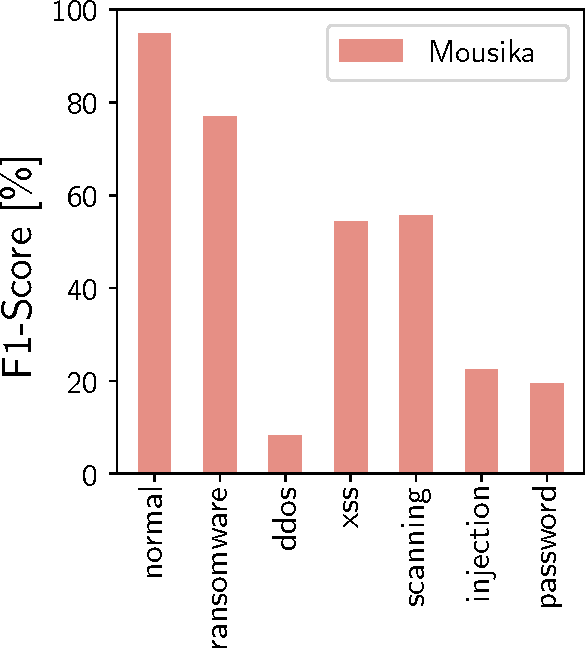
\includegraphics[height=0.225\textwidth]{figures/mousika_score.pdf}
 % }
 % \subfloat[RF(7,3,7)]{
    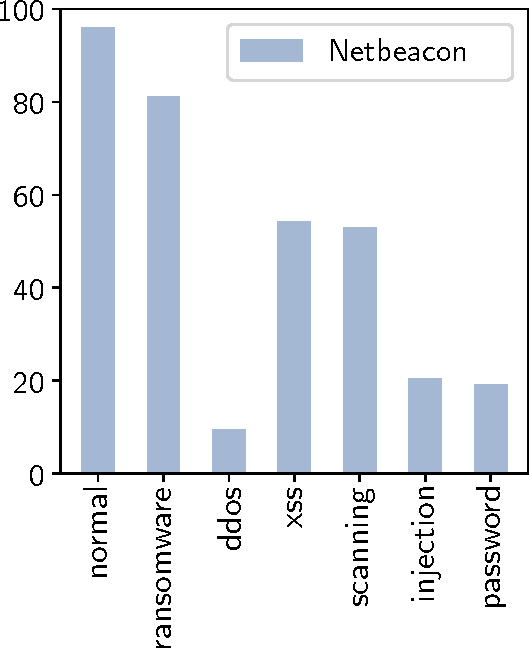
\includegraphics[height=0.225\textwidth]{figures/netbeacon_score.pdf}
 % }
 % \subfloat[RF(9,3,10)]{
    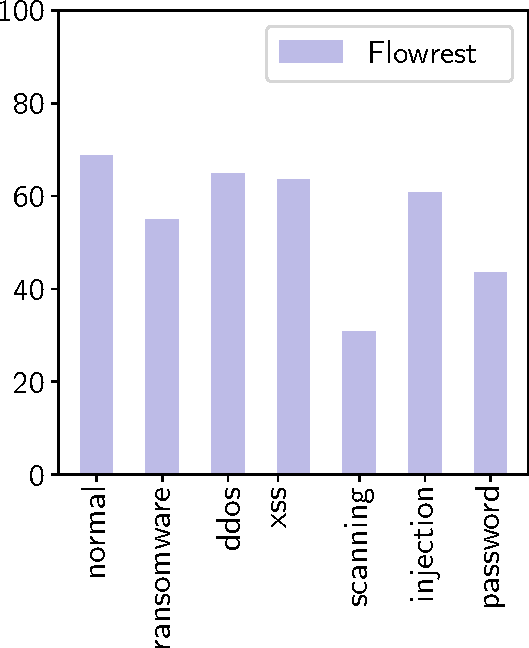
\includegraphics[height=0.225\textwidth]{figures/flowrest_score.pdf}
 % }
 % \subfloat[RF(10,3,9)]{
    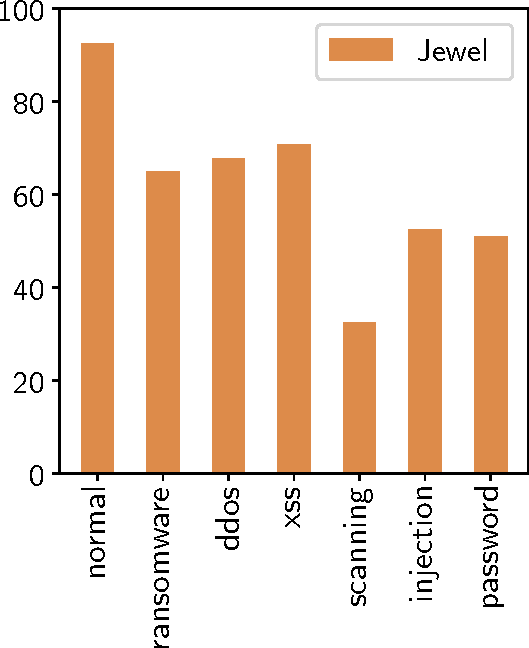
\includegraphics[height=0.225\textwidth]{figures/jewel_score.pdf}

    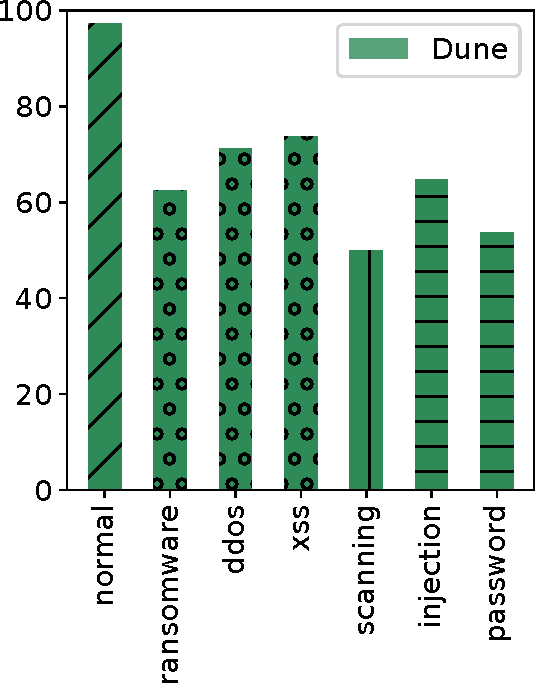
\includegraphics[height=0.225\textwidth]{figures/dune_score_N.pdf}
 }
 \vspace*{-13pt}
 \caption{Per-class F1-score obtained by \name and the benchmarks in ToN-IoT. The hatch in \name indicates the sub-model targeting each class.}
 \label{fig:per_class_accuracy}
 \vspace*{-8pt}
\end{figure*}

\subsection{Small-scale comparative evaluation in hardware}
\label{sub:evaluation-hardware}

We first test the hardware implementation of \name in our experimental platform with a simple linear topology of three Intel Tofino switches as presented in Section~\ref{sec:experimental-setup}. The aim of this part of our evaluation is twofold: first, it lets us prove that \name can be deployed in real-world environments, by verifying its line-rate operation and efficient switch resource usage; second, it allows us to compare the performance of distributed inference against that of traditional monolithic models proposed in the literature in dependable settings.

\textbf{Accuracy.} 
We begin by comparing the performance of distributed inference executed by \name with the benchmarks performing monolithic inference across three different metrics. In order to assess the accuracy of the solutions, we adopt different flavors of the F1 score as detailed in Section~\ref{sub:metrics}.

Table~\ref{tab:F1_scores} shows how \name consistently outperforms all monolithic solutions across all metrics in both use cases, with the exception of the Weighted F1 score in the UNSW dataset, where the PL solution Mousika performs slightly better. The performance improvement of \name, compared to the second-best model in both use cases, ranges from $0.7$\% to $7.5$\% in all metrics, with an average gain of $5.2$\% in the Macro F1 score and an advantage of $20$\% or more over the worst benchmark.
%Given the imbalance in the number of samples across classes in the datasets, the Macro F1 score represents the most challenging metric. Therefore, we prioritize the Macro F1 score and select the best combination of hyperparameters during the model selection phase based on this metric. 

\begin{table}[t]
% \begin{tabular*}{\columnwidth}{@{\extracolsep{\fill}}ccccccl@{}}
\resizebox{\columnwidth}{!}{
\begin{tabular}{@{}ccccccl@{}}
\toprule
\textbf{Dataset}                  & \textbf{F1-Score}      & Mousika & Flowrest & Netbeacon            & Jewel  & \multicolumn{1}{c}{Dune} \\ \midrule
\multirow{3}{*}{\textbf{UNSW}}    & \textbf{Macro}         & 64.921\%  & 40.100\%     & 46.057\%               & 65.718\% &   \textbf{70.263\%}                       \\
                                  & \textbf{Micro}         & 83.568\%  & 41.918\%   & 58.192\%               & 79.132\% &   \textbf{84.291\% }                      \\
                                  & \textbf{Weighted}      & \textbf{83.96\%}   & 40.614\%   & 59.278\%               & 79.776\% &   83.296\%                       \\
\midrule
\multirow{3}{*}{\textbf{ToN-IoT}} & \textbf{Macro}         & 47.099\%  & 55.367\%   & 47.468\% & 61.718\% &  \textbf{67.388\%}                        \\
                                  & \textbf{Micro}         & 42.335\%  & 62,038\%   & 42.380\% & 67.045\% &    \textbf{72.803\%}                      \\
                                  & \textbf{Weighted}      & 37.826\%  & 61.723\%   & 38.024\% & 65.153\% &  \textbf{72.392\%}                        \\ \bottomrule
\end{tabular}
}
\caption{Comparative evaluation of inference accuracy.} %based on \textit{flow-level} metric. 
% The best value on each row is shown in \textbf{black bold} and the second best solution in \textbf{\color{purple}purple bold}.
\label{tab:F1_scores}

\end{table}

% Please add the following required packages to your document preamble:
% \usepackage{multirow}
\begin{table}[]
\resizebox{\columnwidth}{!}{%
\begin{tabular}{lcccccccc}
\toprule
% \multicolumn{1}{c}{\textbf{Dataset}} & \textbf{Resource} & \textbf{Mousika} & \textbf{Flowrest} & \textbf{Netbeacon} & \textbf{Jewel}   & \textbf{DUNE-SW1} & \textbf{DUNE-SW2} & \textbf{DUNE-SW3} \\ \midrule
                            &                   &\multicolumn{4}{c}{Benchmarks}          & \multicolumn{3}{c}{Dune}        \\ \cmidrule(lr){3-6} \cmidrule(l){7-9}
\textbf{Dataset}            & \textbf{Resource} &Mousika & Flowrest & Netbeacon & Jewel  & SW1       & SW2     & SW3       \\ \midrule
\multirow{2}{*}{\textbf{UNSW}}       & \textbf{TCAM}     & 27.80\% & 14.90\%  & 36.10\%   & 15.60\% & 9.40\%  & 8.70\%  & 8.70\%    \\ 
                            & \textbf{SRAM}     & 0.70\%  & 10.10\%  & 13.50\%   & 12.40\% & 17.00\% & 13.00\% & 16.10\%   \\ \midrule
\multirow{2}{*}{\textbf{ToN-IoT}}    & \textbf{TCAM}     & 1.40\%  & 14.20\%  & 20.50\%   & 5.60\%  & 2.40\%  & 5.60\%  & 8.00\%    \\ 
                            & \textbf{SRAM}     & 5.50\%  & 14.70\%  & 19.50\%   & 15.10\% & 12.70\% & 16.40\% & 15.90\%   \\ \bottomrule

\end{tabular}
}
\caption{TCAM and SRAM usage across all models.
}
\label{tab:resource_usage}
\vspace*{-12pt}
\end{table}

\begin{table}[t]
\centering
\resizebox{0.95\columnwidth}{!}{
% %Version 1
% % \begin{tabular}{@{}lcccccrrc@{}}
% % \toprule
% %         & \multicolumn{4}{c}{Benchmarks}          & \multicolumn{4}{c}{Dune}                                                                      \\ \midrule
% % Dataset & Flowrest & Jewel  & Netbeacon & Mousika & SW1                             & \multicolumn{1}{c}{SW2} & \multicolumn{1}{c}{SW3} & TOTAL   \\ \midrule
% % UNSW    & 398,36   & 413,11 & 421,31    & 303,28  & \multicolumn{1}{r}{457,3770492} & 454,0983607             & 435,2459016             & 1137,70 \\ \midrule
% % ToN-IoT & 433,61   & 446,72 & 436,07    & 300,82  & \multicolumn{1}{r}{432,7868852} & 401,6393443             & 434,4262295             & 1183,61 \\ \bottomrule
% % \end{tabular}

% %Version 2
% % \begin{tabular}{@{}lcccccrrc@{}}
% % \toprule
% %         & Flowrest & Jewel  & Netbeacon & Mousika & \multicolumn{4}{c}{Dune}                                                                      \\ \cmidrule(l){7-10} 
% % Dataset &          &        &           &         & SW1                             & \multicolumn{1}{c}{SW2} & \multicolumn{1}{c}{SW3} & TOTAL   \\ \midrule
% % UNSW    & 398,36   & 413,11 & 421,31    & 303,28  & \multicolumn{1}{r}{457,3770492} & 454,0983607             & 435,2459016             & 1137,70 \\ 
% % ToN-IoT & 433,61   & 446,72 & 436,07    & 300,82  & \multicolumn{1}{r}{432,7868852} & 401,6393443             & 434,4262295             & 1183,61 \\ \bottomrule
% % \end{tabular}
% %Version 3
\begin{tabular}{@{}lccccccrrc@{}}
\toprule
                 % & \multicolumn{5}{c}{Benchmarks}          & \multicolumn{4}{c}{Dune}                                                                      \\ \cmidrule(lr){2-6} \cmidrule(l){7-10}
\textbf{Dataset} & No inference & Mousika & Flowrest & Netbeacon & Jewel  &  Dune   \\ \midrule
\textbf{UNSW}    &  852.54 & 871.64  & 966.72   & 989.67    & 981.47  & 1137,70 \\
\textbf{ToN-IoT } & 852.54 & 869.18  & 1001.97   & 1004.43    & 1015.08 & 1183,61 \\ \bottomrule
\end{tabular}
}
\caption{Latency in \textit{ns} of all models across three switches.}
\vspace*{-16pt}
\end{table}


% \begin{table}[]
% \centering
% \resizebox{0.8\columnwidth}{!}{
% %Version 2
% \begin{tabular}{@{}lccccccrrc@{}}
% \toprule
%                  % & \multicolumn{5}{c}{Benchmarks}          & \multicolumn{4}{c}{Dune}                                                                      \\ \cmidrule(lr){2-6} \cmidrule(l){7-10}
% \textbf{Dataset} & No Inference & Mousika & Jewel  &  Dune   \\ \midrule
% \textbf{UNSW}    &  852.54 & 871.64  & 981.47  & 1137,70 \\
% \textbf{ToN-IoT } & 852.54 & 869.18    & 1015.08 & 1183,61 \\ \bottomrule
% \end{tabular}
% }
% \caption{Latency, in \textit{ns}, of \name and the benchmarks across three switches.}
\label{tab:latency}
% \vspace*{-13pt}
% \end{table}

%In addition to demonstrating consistently strong performance across various use cases, it is crucial to avoid favoring or neglecting any particular class, thereby preventing the model from overlooking important but less frequent events, and contributing to fairer and more comprehensive outcomes.
Figure~\ref{fig:per_class_accuracy} breaks down the F1 score on a per-class basis for each solution. Mousika and NetBeacon exhibit a significant imbalance across classes, whereas NetBeacon and Jewel have more balanced performance yet still encounter challenges in accurately classifying certain classes compared to others. \name, on the other hand, shows a more balanced accuracy compared to other solutions, except for the class representing benign traffic, which is best classified by all the solutions. \name achieves a more homogeneous accuracy across all classes by breaking down the main inference task into dedicated sub-models, as represented with different hatches, ensuring that each class receives adequate attention.

\textbf{Resource usage.} Due to the constraints of programmable network hardware, evaluating resource usage is essential. Table~\ref{tab:resource_usage} shows the SRAM and TCAM resource usage of all the benchmarks and \name in both use cases. 
We show the resource consumption of all the switches in which the sub-models are deployed. In UNSW, we implement two sub-models per switch, while in ToN-IoT, we implement two models in the last switch and one in the other two. In terms of SRAM consumption, Mousika is the most efficient as it does not require flow-level management. There is no general gain or loss in the consumption across switches hosting distributed models compared to FL and hybrid solutions. However, given the fact that multiple models are typically deployed per switch, the SRAM consumption of individual sub-models is lower than that of monolithic models, except for Mousika. The reason is that we utilize only one register if multiple sub-models use the same FL features in each switch.
Regarding TCAM, the scarcest resource in programmable switches, \name shows, in UNSW, lower consumption across all switches compared to other benchmarks, despite deploying two sub-models per switch. In ToN-IoT, besides Mousika, which consumes less but brings a lower score, the TCAM usage in the switches running a single model is lower than the monolithic solutions.

\textbf{Latency.} Finally, we calculate the end-to-end latency of the benchmarks and \name in all use cases across three switches, in Table~\ref{tab:latency}.
The \textit{no inference} case is a baseline where packets are simply forwarded by the switches.
For monolithic models, packets passing through the first switch incur both forwarding and inference latency, while packets traversing subsequent switches are subject only to forwarding latency. In \name, all switches combine the latency of forwarding and inference.
%Considering that the packets traverse all the switches, each introducing forwarding latency, distributing inference logic into each switch in \name introduces marginal additional latency compared to a monolithic model, where inference is performed only at the first switch, as depicted in Table~\ref{tab:latency}.
The results show how \name realizes line-rate inference with a negligible added delay of around $100$~ns per switch with respect to a pure forwarding operation. This delay is on par with that of solutions with a flow-management functionality.

%Overall, \name proves that the distributed inference can go beyond what a monolithic model can achieve with a lower resource usage per switch.

\subsection{Large-scale scalability assessment via emulation}
\label{sub:evaluation-software}

We now consider the software implementation of \name and employ the emulation environment to run additional experiments.
The aim of these tests is twofold: first, they allow proving the credibility of the software version of \name by juxtaposing its performance in a \texttt{mininet} topology against that of the hardware implementation running on an equivalent network of real-world switches; second, they let us explore the scalability of \name to large topologies with complex routing.
The evaluation is here limited to the ToN-IoT use case since, unlike the UNSW-IoT task, its inference process does not rely on time-based features that, as explained in Section~\ref{sub:software}, are not properly handled by the bmv2 model.

\begin{figure}
    \centering
    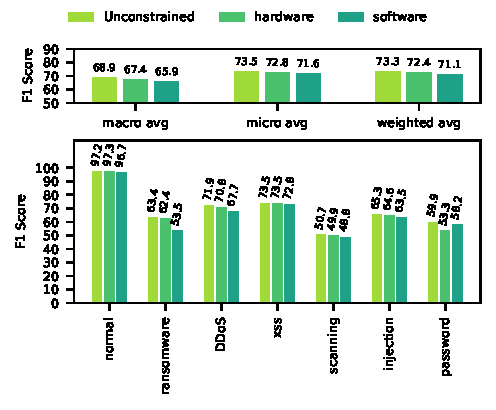
\includegraphics[]{figures/sw_evaluation_1.pdf}
    \vspace{-8pt}
    \caption{Performance comparison between \name software- and hardware-based implementations in the ToN-IoT use case.
    The unconstrained results are for the best possible ML model running on Python in a high-end server.
    % , which is unaffected by all complexities of user-plane operations
    % Linear and Fat tree are bmv2-based.
    % \mf{I would split these plots into two: one figure identical to this one with `python' (renamed to `Unconstrained'), `hw-linear' (renamed to `hardware'), and `sw-linear' (renamed to `software'); one table with the numerical F1 scores of `sw-linear' (renamed to `Linear') and `sw-fattree' (renamed to `Fat Tree'). Also, in the figure I would add numbers on top of the bars to make results more understandable}.
    }
    \label{fig:hw_sw_comparison}
    %\vspace*{-16pt}
\end{figure}

% \begin{table}[h]
% \centering
% \caption{Lorem Ipsum}
% \label{tab:f1_comparison}
% \begin{tabular}{lccccccc}
% \toprule
% % Unconstrained & Unconstrained & Unconstrained & Unconstrained & Unconstrained & Unconstrained & Unconstrained \\
%  & normal & ransomware & ddos & xss & scanning & injection & password & Macro Avg.\\
% \midrule
% % Unconstrained & 0.972 & 0.634 & 0.719 & 0.735 & 0.507 & 0.653 & 0.599 \\
% Linear & 0.967 & 0.535 & 0.677 & 0.728 & 0.488 & 0.635 & 0.582 \\
% Fat Tree & 0.970 & 0.583 & 0.662 & 0.723 & 0.481 & 0.605 & 0.549 \\
% \bottomrule
% \end{tabular}
% \end{table}
\begin{table}
\centering
\caption{F1 score comparison for the ToN-IoT use case when \name is deployed in a 4-node linear topology and a 36-node Fat Tree topology, both emulated in software.}
\label{tab:f1_comparison}
\begin{tabular}{lccr}
\toprule
Class & Linear & Fat Tree & Deviation \\%Deviation (\%) \\
\midrule
Normal & 96.7 & 97.0 & 0.3 \\ %0.31 \\
Ransomware & 53.5 & 58.3 & 4.8 \\ %8.97 \\
DDoS & 67.7 & 66.2 & 1.5 \\ %2.21 \\
XSS & 72.8 & 72.3 & 0.5 \\ %0.69 \\
Scanning & 48.8 & 48.1 & 0.7 \\ %1.43 \\
Injection & 63.5 & 60.5 & 3.0 \\ %4.72 \\
Password & 58.2 & 54.9 & 3.3 \\ %5.67 \\
\midrule
\textbf{Macro} & 65.8 & 65.3 & 0.5 \\ %0.76 \\
\textbf{Micro} & 71.5 & 70.4 & 1.1 \\ %1.54 \\
\textbf{Weighted} & 71.1 & 69.8 & 0.3 \\ %1.83 \\
\bottomrule
\end{tabular}
\end{table}

\begin{table*}[h]
\centering
\caption{Results of \name ML sub-model planning for representative Fat-Tree sizes in the ToN-IoT use case. The communication direction is East-West, with each ingress leaf communicating with one egress leaf. The number of leafs and spines is per pod, one of which is the egress pod. The `nodes' column reports the number of nodes (\ie switches) running ML sub-models over the total number of nodes in the network, and the `\%' column that ratio expressed as a percentage.}
\label{tab:planner_perf}
\begin{tabular}{cccccccll}
\toprule
DC Size & Pods & Leafs & Spines & Super spines & Paths & Nodes & \% & Notes \\
\midrule
XS & 2  & 2  & 2  & 1 & 4    & 8/10  & 80\% & Tiny DC: testing, labs \\
S  & 4  & 4  & 3  & 1 & 12   & 19/31 & 61\% & Small DC: edge, small enterprise \\
M  & 8  & 6  & 4  & 2 & 192  & 46/88 & 52\% & Medium DC: medium enterprise, small offsite \\
L  & 16 & 8  & 5  & 2 & 960 & 98/218 & 45\% & Large DC: large enterprise, medium offsite \\
XL & 32 & 10 & 7  & 4 & 3100 & 262/572 & 45\% & Very large DC: hyperscalers \\
\bottomrule
\end{tabular}
\vspace*{-13pt}
\end{table*}


\textbf{Validation of the software implementation.}
Figure~\ref{fig:hw_sw_comparison} compares the accuracy of the two versions of \name, \ie hardware and software, once deployed in a  linear topology. Such a topology is realized with 3 real-world Intel Tofino switches for the hardware version of \name and with 4 switches emulated in \texttt{mininet} for the software version.

The various F1 scores are also placed side by side with those obtained by the unconstrained ML model trained in stage \numO{1} of the \name pipeline in Section~\ref{sec:name-control-plane}, which runs on a high-end server using Python libraries and provides an upper bound to the inference performance.
We observe that the hardware and software implementations show very close accuracy, with a discrepancy of $0.1$ percent points in the averaged F1 scores in favor of the hardware version (top plot); even when looking at class-level F1 scores, we see differences between $0$ and $9$ percent points (bottom plot). These relatively small differences are mainly caused by the high latency of bmv2 cross-plane communications discussed in Section~\ref{sub:software}, which causes delay and losses in digests, hence additional flow collisions in the switches.
Moreover, both implementations of \name have close performance to the best case represented by the unconstrained ML model running on Python, which is unaffected by all complexities of user-plane operations.

%The bottom part of Figure~\ref{fig:hw_sw_comparison} disaggregates the F1 score across the eight classes of the ToN-IoT use case. The result highlights how the behavior of the hardware and software implementations is very consistent and always close to that of the original unconstrained ML model.

\textbf{Operation in a large Fat Tree topology.}
We now assess the capability of \name to operate in large real-world networks. To this end, we rely on the software implementation of our framework and deploy it in an emulated Fat Tree topology with 16 leaf and 16 spine switches organized into 4 pods, which are in turn connected through 4 super-spine nodes.
We inject traffic flows from the ToN-IoT use case into the leaf nodes, as explained in Section~\ref{sub:topologies}, and run the distributed inference task across the whole network so that every flow in the Fat Tree network is classified by \name. 
Table \ref{tab:f1_comparison} compares the resulting F1 scores to those recorded in a simple four-switch linear topology: deviations are small, in the [$0.3$--$1.1$] range when considering average metrics and in the [$0.3$--$4.8$] range for individual classes.
As discussed in Section~\ref{sub:topologies}, the differences are primarily caused by higher flow collisions in the Fat Tree, yet we deem them acceptable considering the much larger size and higher complexity of the target network.

Finally, we assess the efficiency of \name in distributing the inference process in Fat Tree topologies. To this end, we consider the sequenced ML sub-models of the ToN-IoT use case returned by stage \numO{5} of the pipeline in Section~\ref{sec:name-control-plane}; we then run the planning stage \numO{6} to deploy such models into Fat Tree networks that follow the architecture in Figure~\ref{fig:clos_topology} and have increasing size.
Table \ref{tab:planner_perf} reports the number of RFs required to process the ToN-IoT workload in topologies representative of typical data center networks, from private edge facilities to hyperscalers.
It is apparent how the efficiency of \name increases with the network size, as larger topologies present a wider decision space and more opportunities for optimization of the placement of sub-models. Ultimately, the result proves the effectiveness of \name in limiting the resources used by the inference process not only locally at each switch but also globally throughout the target network infrastructure.

\section{Conclusions}
\label{sec:conclusions}

We propose \name, the first framework that automatically decomposes unconstrained user-plane classification models into simpler sub-models and determines their optimal placement across programmable switches, enabling deployment in network topologies of varying complexity. Results demonstrate that \name is topology-aware and can adapt to arbitrary network topologies of varying sizes.
Extensive experiments show that \name yields higher accuracy than traditional single-device approaches, with lower resource usage and comparable delay.
The authors have provided public access to their code at~\cite{code-dune}.


%Strong interest in data plane FL. Neural networks yield high accuracy but their complexity is high making them difficult to implement in the switch. Decision tree-based models have proven to be easier to implement in switches due to their simple structure. 
%Previous studies did not report memory usage as a proportion of the total switch resources, making it impossible to judge on the viability of the solutions.

%%
%% The acknowledgments section is defined using the "acks" environment
%% (and NOT an unnumbered section). This ensures the proper
%% identification of the section in the article metadata, and the
%% consistent spelling of the heading.



% if have a single appendix:
%\appendix[Proof of the Zonklar Equations]
% or
%\appendix  % for no appendix heading
% do not use \section anymore after \appendix, only \section*
% is possibly needed

% use appendices with more than one appendix
% then use \section to start each appendix
% you must declare a \section before using any
% \subsection or using \label (\appendices by itself
% starts a section numbered zero.)
%


% \appendices
% \section{}
% Appendix one text goes here.

% you can choose not to have a title for an appendix
% if you want by leaving the argument blank
% \section{}
% Appendix two text goes here.

% --- for the camera ready only
% use section* for acknowledgment
% \section*{Acknowledgments}
% This work has received funding from the Smart Networks and Services Joint Undertaking (SNS JU) under the European Union’s Horizon Europe research and innovation programme under grant agreement no. 101139270 ``ORIGAMI''. This work was also funded by the CHIST-ERA grant no. CHIST-ERA-20-SICT-001 ``ECOMOME'', via grant PCI2022-133013 of Agencia Estatal de Investigaci\'on.

% Can use something like this to put references on a page
% by themselves when using endfloat and the captionsoff option.
\ifCLASSOPTIONcaptionsoff
  \newpage
\fi


% trigger a \newpage just before the given reference
% number - used to balance the columns on the last page
% adjust value as needed - may need to be readjusted if
% the document is modified later
%\IEEEtriggeratref{8}
% The "triggered" command can be changed if desired:
%\IEEEtriggercmd{\enlargethispage{-5in}}

% references section

% can use a bibliography generated by BibTeX as a .bbl file
% BibTeX documentation can be easily obtained at:
% http://mirror.ctan.org/biblio/bibtex/contrib/doc/
% The IEEEtran BibTeX style support page is at:
% http://www.michaelshell.org/tex/ieeetran/bibtex/
%\bibliographystyle{IEEEtran}
% argument is your BibTeX string definitions and bibliography database(s)
%\bibliography{IEEEabrv,../bib/paper}
%
% <OR> manually copy in the resultant .bbl file
% set second argument of \begin to the number of references
% (used to reserve space for the reference number labels box)
\balance
% \bibliographystyle{IEEEtran} 
\bibliographystyle{unsrt2authabbrvpp}
% \bibliographystyle{jabbrv_ieeetr}
% \newpage
% 
\bibliography{references}

% \input{appendix}

% biography section
% 
% If you have an EPS/PDF photo (graphicx package needed) extra braces are
% needed around the contents of the optional argument to biography to prevent
% the LaTeX parser from getting confused when it sees the complicated
% \includegraphics command within an optional argument. (You could create
% your own custom macro containing the \includegraphics command to make things
% simpler here.)
%\begin{IEEEbiography}[{\includegraphics[width=1in,height=1.25in,clip,keepaspectratio]{mshell}}]{Michael Shell}
% or if you just want to reserve a space for a photo:

%\vspace*{-30pt}
%\begin{IEEEbiography}[{\includegraphics[width=1in,height=1.25in,clip,keepaspectratio]{figures/biophotos/media-file-beyza-butun-scaled-e1661346526450-450x550.jpg}}] {Beyza~B\"{u}t\"{u}n} (Student Member, IEEE) is a Ph.D. student in the Networks Data Science Group at IMDEA Networks Institute in Madrid, Spain. She is part of the project ECOMOME, which aims to model and optimise the energy consumption of networks. She is also a Ph.D. student in the Department of Telematics Engineering at Universidad Carlos III de Madrid, Spain. She holds a bachelor's and master's degree in Computer Engineering from Middle East Technical University in Ankara, Turkey. During her master's, she worked on the optimal design of wireless data center networks. Beyza's current research interest is in-band network intelligence and energy consumption optimization in the data plane.
% \begin{IEEEbiographynophoto}
% {Beyza~B\"{u}t\"{u}n} (Student Member, IEEE) is a PhD student at IMDEA Networks Institute and in the Department of Telematics Engineering at Universidad Carlos III de Madrid, Spain. She holds bachelor's and master's degrees in Computer Engineering from Middle East Technical University, Turkey. Beyza's research interests are user-plane intelligence and energy efficiency.
% \end{IEEEbiographynophoto}

%\vspace*{-30pt}
%\begin{IEEEbiography}[{\includegraphics[width=1in,height=1.25in,clip,keepaspectratio]{figures/biophotos/media-file-michele-gucciardo-scaled-e1615285554193-450x550.jpg}}] {Michele Gucciardo} (Member, IEEE) is a Postdoctoral Researcher at IMDEA Networks Institute. He received the B.Sc. degree from Politecnico di Milano, Italy, in 2008, and the M.Sc. degree from the University of Palermo, Italy, in 2013, all in telecommunications engineering. He later received the Ph.D. degree in information and communication technologies from the University of Palermo in 2020. He has also been a Visiting Researcher at the TIM Labs, Turin, Italy, and at the IMDEA Networks Institute, Madrid, Spain, in 2018 and 2019. His research interests have been focused on the experimental evaluation of emerging the IoT technologies, software defined infrastructures, programmable networks, data plane inference, machine learning in 5G, and computational offloading in wireless networks.
% \begin{IEEEbiographynophoto}
% {Michele Gucciardo} (Member, IEEE) is a Postdoctoral Researcher at IMDEA Networks Institute. He received a B.Sc. degree from Politecnico di Milano in 2008, and M.Sc. and Ph.D. degrees from the University of Palermo in 2013 and 2020. He was a visiting Researcher at TIM Labs in 2018. His research interests are on the experimental evaluation of network systems including software-defined and programmable infrastructures.
% \end{IEEEbiographynophoto}
%
%\vspace*{-30pt}
%\begin{IEEEbiography}[{\includegraphics[width=1in,height=1.25in,clip,keepaspectratio]{figures/biophotos/imdea-2022_marco-fiore_cut.jpg}}] (Senior Member, IEEE) is a Research Professor at IMDEA Networks Institute and CTO at Net AI Tech Ltd. He received M.Sc. degrees from University of Illinois at Chicago, IL, USA (2003), and Politecnico di Torino, Italy (2004), a Ph.D. degree from Politecnico di Torino (2008), Italy, and a Habilitation a Diriger des Recherches (HDR) from Universite de Lyon, France (2014). He held tenured positions as Maitre de Conferences (Associate Professor) at Institut National des Sciences Appliquees (INSA) de Lyon, France (2009-2013), and Researcher at Consiglio Nazionale delle Ricerche (CNR), Italy (2013-2019). He has been a visiting researcher at Rice University, TX, USA (2006-2007), Universitat Politecnica de Catalunya (UPC), Spain (2008), and University College London (UCL), UK (2016-2018). Dr. Fiore is a senior member of IEEE, and a member of ACM. He was a recipient of a European Union Marie Curie fellowship and a Royal Society International Exchange fellowship. He leads the Networks Data Science group at IMDEA Networks Institute, which focuses on research at the interface of computer networks, data analysis and machine learning.
% \begin{IEEEbiographynophoto}
% {Marco Fiore}
% (Senior Member, IEEE) is a Research Professor at IMDEA Networks Institute, where he leads the Networks Science Data group, and CTO at Net AI Tech Ltd, a network intelligence start-up. He received M.Sc. degrees from University of Illinois at Chicago and Politecnico di Torino, a Ph.D. degree from Politecnico di Torino, and an habilitation from Universit\'e de Lyon.
% He held tenured academic positions in France and Italy, and was a visiting researcher in the USA, Spain and UK.
% His research interests are at interface of computer networks, data analysis and machine learning.
% \end{IEEEbiographynophoto}
%\vfill

% \balance
% % if you will not have a photo at all:
% \begin{IEEEbiographynophoto}{John Doe}
% Biography text here.
% \end{IEEEbiographynophoto}

% insert where needed to balance the two columns on the last page with
% biographies
%\newpage

% You can push biographies down or up by placing
% a \vfill before or after them. The appropriate
% use of \vfill depends on what kind of text is
% on the last page and whether or not the columns
% are being equalized.

%\vfill

% Can be used to pull up biographies so that the bottom of the last one
% is flush with the other column.
%\enlargethispage{-5in}


% that's all folks
\end{document}


